%This is the third chapter of the dissertation

%The following command starts your chapter. If you want different titles used in your ToC and at the top of the page throughout the chapter, you can specify those values here. Since Columbia doesn't want extra information in the headers and footers, the "Top of Page Title" value won't actually appear.

\pagestyle{cu}
\graphicspath{{./Chapter3/Figures/}}
\chapter[The XENON1T Dark Matter Search][The XENON1T Dark Matter Search]{The XENON1T Dark Matter Search}

% https://arxiv.org/pdf/1801.07231.pdf for electron emission from wires


XENON1T is the third generation experiment of the XENON collaboration.  With a fiducial mass of $> 1000\ \mathrm{kg}$ it is the first
liquid xenon dark matter detector to reach the ton-scale era of DM detection.  Its large target mass and low radioactive background
makes it the most sensitive detector to spin-independent WIMPs.

In this chapter I describe the XENON1T experiment (\secref{sec:xenon1t_detector}) and give the results of the second science run
(\secref{sec:xenon1t_sr1}).

Lots of good info in Aprile2017b (instrument paper).

\section{The XENON1T Detector}
\label{sec:xenon1t_detector}




\subsection{PMTs}
\label{subsec:xenon1t_pmts}
A total of 248 Hamamatsu R11410-21 PMTs are installed in XENON1T.  The 127 PMTs in the top array are placed in a radial distribution to
maximize resolution of $r$ position reconstruction (\secref{subsec:det_char_position_reconstruction}).  The 121 in the bottom array
are packed as densely as possible to maximize light
collection.  The R11410 window is 76.2 mm in diameter and the photocathode yields an average QE to 178 nm of 34.5\% with 2.8\%
standard deviation (\citeref{Aprile2017b, Barrow2017}).  The high QEs result from preselecting PMTs with $\mathrm{QE} > 28\%$ for
screening.

PMTs with the highest QE are placed in the bottom array while those with the lowest are stationed along the outside of the
top.  The difference in arrangement is strategic.  Due to liquid xenon's relatively large dielectric constant (1.95) an S1 will
often reflect off the surface and be redirected towards the bottom of the TPC.  For low-energy events - the relevant range for WIMP DM
searches - a nuclear recoils may only emit a small number ($\lesssim 100$) of photons, many of which never reach the PMTs.  Thus it is
most advantageous to position those with the highest quantum efficiency in the region most likely to see scintillation from an
S1.  Likewise, S2s easily produce enough scintillation to be observed by both arrays.  Therefore the QE of the top PMTs is comparatively
unimportant, and may even be advantageous for larger S2s where saturation can occur.  The layout of the PMTs with respect to QE is shown
in \figref{fig:xenon1t_pmt_qe}.

\begin{figure}
\centering
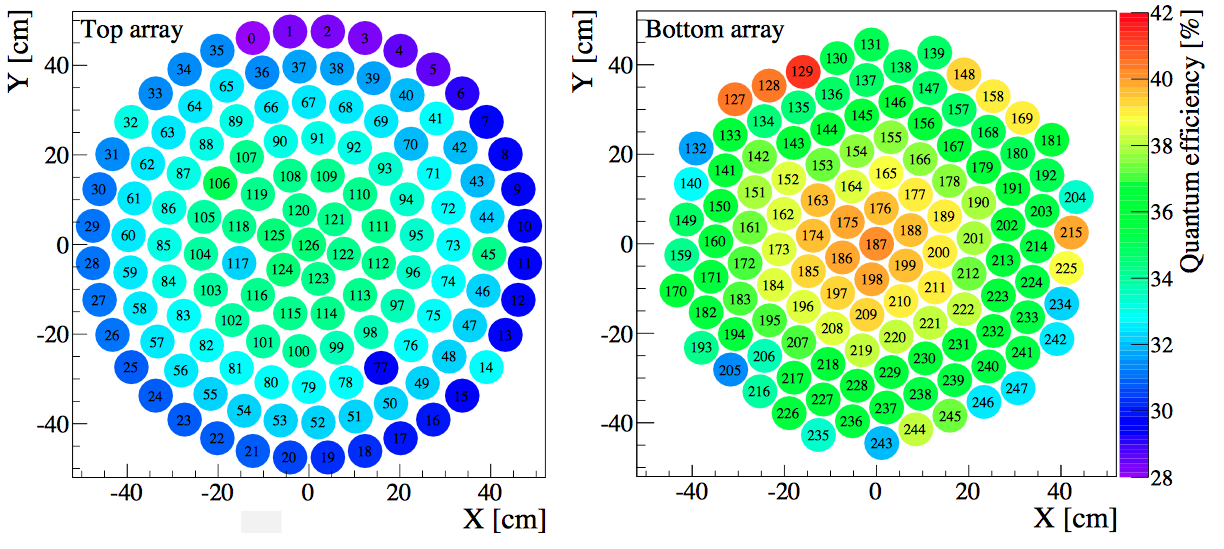
\includegraphics[width=\textwidth]{PMTQuantumEfficiency}
\caption{Quantum efficiency of top (left) and bottom (right) PMT arrays.  PMTs with highest QE are placed in the center of the bottom
array to maximize light collection while those with the lowest are placed in the outer region of the top.  Image credit:
\citeref{Aprile2017b}.}
\label{fig:xenon1t_pmt_qe}
\end{figure}

The two PMT arrays are supported by oxygen-free high thermal conductivity (OFHC) copper, with holes in which the PMTs are placed.  The
copper is then covered with polytetrafluoroethylene (PTFE) on the TPC-facing sides.  Screening meshes are situated between the bottom
array and cathode as well as the anode and top array.  Each can be biased to minimize electrical interference between the
phototubes and the drift and extraction fields.  While \citeref{Baudis2013} showed normal operation of R11410 PMTs at
$\geq 11\ \mathrm{kV\ cm^{-1}}$ the expected voltage for the cathode was $10-100\ \mathrm{kV\ cm^{-1}}$ and decreasing the stress on the
phototubes is likely to be beneficial longterm.  The finished arrays are shown in \figref{fig:xenon1t_pmt_array}.

\begin{figure}
    \centering
    \begin{subfigure}[t]{0.45\textwidth}
        \centering
        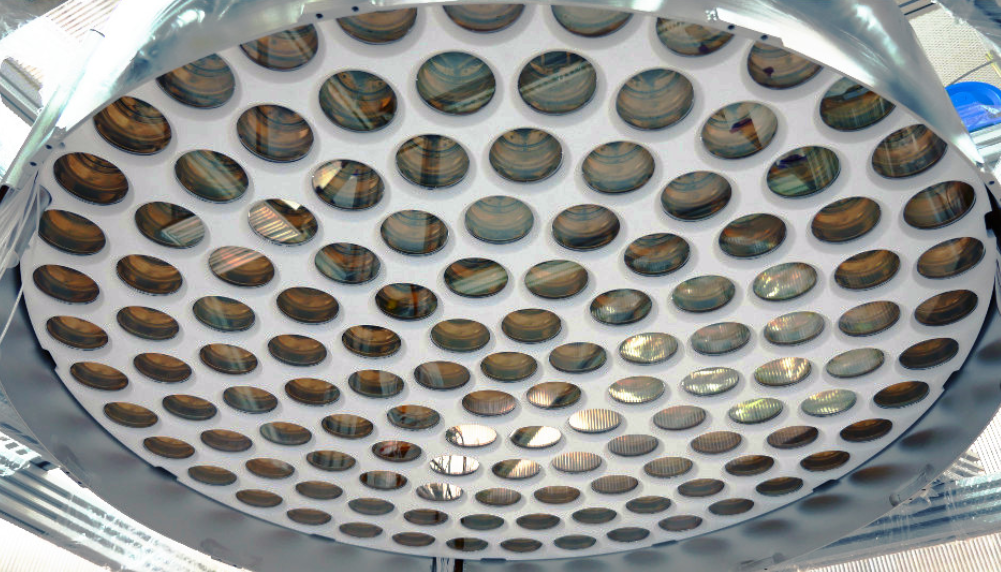
\includegraphics[width=\textwidth]{PMTTopArray}
    \end{subfigure}%
    \begin{subfigure}[t]{width=textwidth}
        \centering
        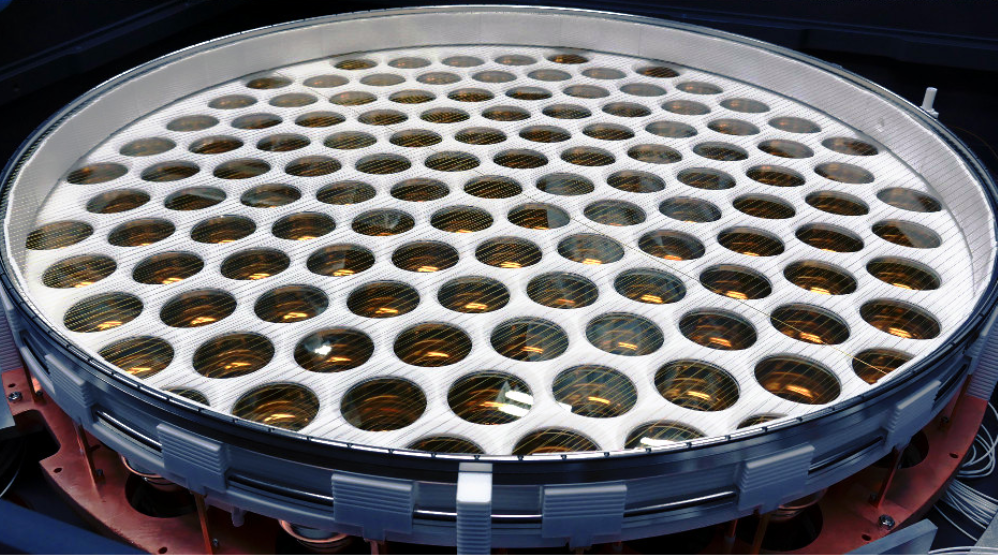
\includegraphics[height=4.5cm]{PMTBottomArray}
    \end{subfigure}
    \caption{XENON1T top (left) and bottom (right) PMT arrays.  Top PMTs are installed inside the diving bell in a radial distribution
    to minimize uncertainty in radial position reconstruction.  Bottom PMTs are installed below the cathode and screening mesh that
    limits interference between the PMT and cathode electric fields, both of which can be seen.  They are packed tightly
    together to maximize lightcollection.  Image credit: \citeref{Aprile2017b}.}
	\label{fig:xenon1t_pmt_array}
\end{figure}

\begin{figure}
\centering
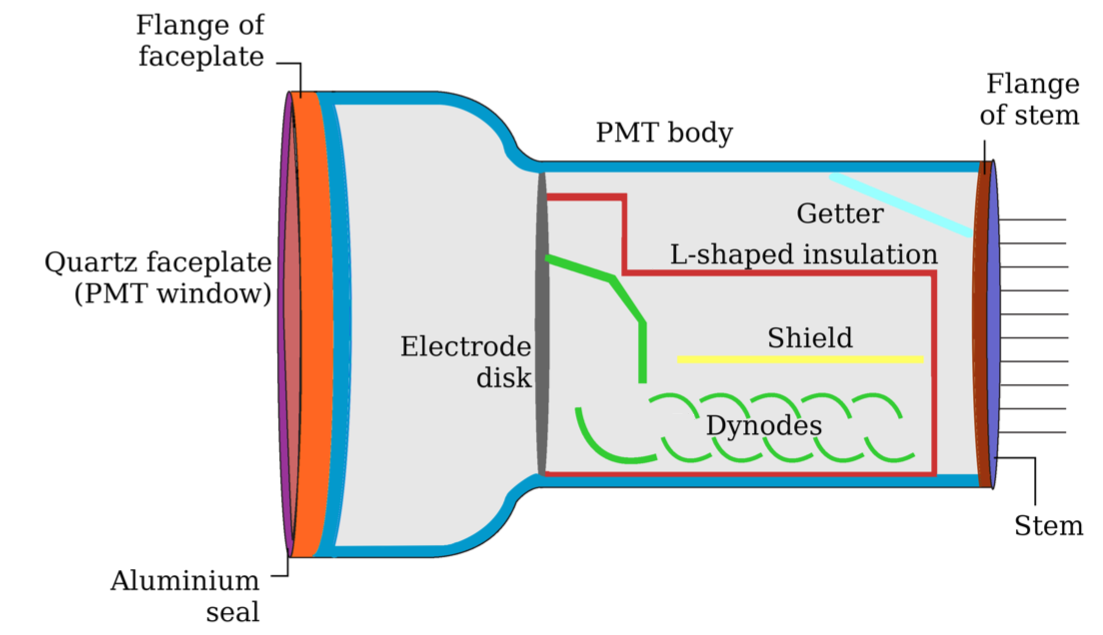
\includegraphics[width=0.8\textwidth]{PMTSchematic}
\caption{Schematic of the R11410-21 PMT.}
\label{fig:xenon1t_hamamatsu_pmt}
\end{figure}

The R11410-21 has 12 dynodes following the focusing electrode disk.  The first dynode is the largest and extends to the electrode to
maximize the probability of capturing photoelectrons.  A schematic can be be seen in \figref{fig:xenon1t_hamamatsu_pmt}.  The electrode,
dynode, and shield are stainless steel and are insulated with L-shaped quartz plates.  The window is
also made of quartz, since it is transparent to vacuum ultraviolet (VUV) photons.  Deposited on it is a low-temperature bialkali
photocathode.  The window is fixed with an aluminum seal to the faceplate flange, which along with the stem flange is constructed from
Kovar.  Because of the PMT body's large mass (71\% of total Kovar, 35\% of total) a low-\ce{^{60}Co} Kovar is chosen.  Finally, to insulate
the connections to each dynode the stem is ceramic.

Because radioactivity limits the fiducial volume and increases the event rate, making accidental coincidence and outlier events more
likely, XENON and Hamamatsu worked together to develop a highly radio-pure PMT.  There were several iterations of the R11410 model before
the R11410-21 was determined to be adequate.  Nearly all the \ce{^{137}Cs} and \ce{^{60}Co} comes from the Kovar, though the \ce{^{137}Cs}
content is negligible and the \ce{^{60}Co} is 3-10 times lower than older models.  The remaining screened isotopes, \ce{^{238}U},
\ce{^{228}Th}, \ce{^{228}Ra}, \ce{^{226}Ra}, and \ce{^{40}K}, are dominated by the ceramic stem (\citeref{Aprile2015}).  Unfortunately a
material that is more radio-pure and can insulate the dynode connections has not been found.  Sapphire was used in an iteration but
ultimately showed any improvement was minimal.

The dark count rate, or the number of signals per second above a threshold without a light source, is an important property to
characterize.  At ambient temperatures the primary cause is thermal electrons that scale with PMT voltage.  This becomes subdominant at
cryogenic temperatures to electron field emission and radioactivity (internal and external) as well as cosmic rays.  In a detector such
as XENON1T higher dark count rates make accidental coincidence more likely, which produces fake additional background and in the worst case
can place fake events in the signal region.  Because the rate is dependent on the threshold it can effectively be tuned.  However, because
for DM search we would like as low of a threshold as possible, choosing PMTs with low dark count rate is essential.

Another problematic feature is light emission from the phototube itself, where light is created inside the PMT and escapes through the
window.  It has been observed to mainly occur in one of two ways.  The first is through a discharge of intense light that can last for
several seconds.  This so-called ``flash" is bright enough to be easily observable to itself and by PMTs that are facing its
window.  However, the intensity can be so strong that it can take anywhere from several minutes to several hours for them to
recover.  Because they seem to occur spontaneously and are not well understood it is impossible to predict when a flash will occur.

The second variety is a subtle but often continuous stream of light.  Known as ``micro light emission" it is considerably harder to
identify.  Doing so requires facing two phototubes towards one another and measuring the dark rate of each one with and without the other
on.  The level of emission increases with temperature and bias voltage.  Keeping the PMTs at cryogenic temperatures during DM runs reduces
such effects, and voltages can be lowered to help further.  Still, if micro light emission continues the PMT cannot be used as it risks
contaminating the detected light from the true event population.

Directly following the pulse of a PMT hit a secondary pulse may occur.  Known as afterpulses, they can occur within 10s of
nanoseconds.  This can make them difficult to resolve from true pulses - especially S2s - that can have widths of several
microseconds.  However, they are an inevitable side effect when using PMTs so characterizing them properly is important.  There are three
mechanisms known to cause afterpulses.

The first is elastic scattering of the photoelectron with the first dynode, freeing \electron that shortly return to the dynode.  This
prompts afterpulses in the range of a few to tens of nanoseconds.  A second kind is thought to stem
from dark noise and single electrons but is not well understood.  It has a relatively uniform distribution in delay time up to several
microseconds.  Both of these afterpulses have relatively small areas of $\lesssim 2\ \mathrm{PE}$.

A photoelectron may occasionally ionize residual gas inside the PMT along its trajectory to the first dynode.  The molecule then drifts
towards the photocathode, expelling additional electrons.  The number of newly ejected electrons (area of afterpulse) depends
on the ion and the position of ionization.  The responsible ion can be determined by calculating the time between the true pulse and
afterpulse.  For R11410-21 this gives

\begin{equation}
\delta t_{\mathrm{ap}} = \frac{\pi}{4} \sqrt{\frac{2 m}{q V_{0}}} L
\end{equation}

where $\delta t_{\mathrm{ap}}$ is the delay time, $m$ and $q$ are the ion's mass and charge, and $V_{0}$ and $L$ are the potential
difference and length between the photocathode and first dynode (see \citeref{Barrow2017} for details).  Note that $\delta t_{\mathrm{ap}}$
does not depend on where the ionization occurred.  Thus, if we know the time between the true and afterpulse the ion - or more specifically
charge to mass ratio - can be calculated.  Pulse time differences range from several hundred nanoseconds to several microseconds.  These
correspond to the ``lines" in \figref{fig:xenon1t_pmts_ap} that extend to larger afterpulses.  The short timescales of S1s make them
unlikely to be grouped with an afterpulse, though for S2s this is more likely.

\begin{figure}
\centering
\includegraphics[width=\textwidth]{Afterpulse}
\caption{Afterpulses for one of the PMTs from XENON1T.}
\label{fig:xenon1t_pmts_ap}
\end{figure}

Because it is not possible to remove all residual gas any PMT will suffer from some ionization-based afterpulsing.  A better vacuum
corresponds to fewer afterpulses and a healthier PMT in general.  If the concentration of gas in the PMT vacuum were to increase it would
escalate the afterpulse rate.  Therefore if when using in xenon the Xe peaks grow over time the PMT most likely has a leak and should
be removed, as continued worsening of the vacuum will lead to deterioration and inability to operate the PMT.  All PMTs were tested before
being installed in XENON1T.  73 were rejected and replaced: 12 due to high dark count rates, 53 for light emission, and 8 for
afterpulsing.

The transit time (TT) is the time between the freed photoelectron and the arrival of the electron avalanche at the anode.  Variations in
the photoelectron's initial position as well as emitted velocity and angle cause deviations in the TT, which is characterized by the
transit time spread (TTS).  Because an event is observed by many PMTs the TTS quantifies how close together there signals should be.  Thus
smaller TTSs lead to a smaller integration window, decreasing accidental coincidence.  The TTS for all R11410-21 PMTs was measured, giving
a mean of $9.1 \pm 1.3\ \mathrm{ns}$ - a fraction of an S1.

An additional six Hamamatsu R8520 PMTs reside in LXe outside the TPC near the top electrode for studying calibrations.  These PMTs have
been used in a number of LXe TPCs including XENON100, the predecessor to XENON1T (\citeref{Goetzke2017}, see \citeref{Aprile2012a} for
details on XENON100).




\subsection{TPC}
\label{subsec:xenon1t_tpc}
The XENON1T time projection chamber is cylindrical with a 96.9 cm height and 47.9 cm diamater.  It encloses a target mass of 2.0 tons where
light and charge can be measured.  A schematic is shown in \figref{fig:xenon1t_tpc_tpc}.  The interior of the vertical wall consists of 24
PTFE panels that were treated with diamond tools to
maximize VUV reflectivity.  Each interlocks with adjacent panels to achieve light-tightness, and the system is designed so that despite
the high thermal expansion coefficient the radius does not contract when lowered to $-96^{\circ}\ \mathrm{C}$.  Outside the PTFE are 74
field shaping rings made of low-radioactivity OFHC copper, each with a cross section of ${\sim} 10 \times 5\ \mathrm{mm^{2}}$.  They are
supported by 18 PTFE pillars stationed around the circumference.  Two redundant
chains connect adjoining rings via $5\ \mathrm{G \Omega}$ resistors, each with a $25\ \mathrm{G \Omega}$ resistor between the bottom and
cathode.

\begin{figure}
\centering
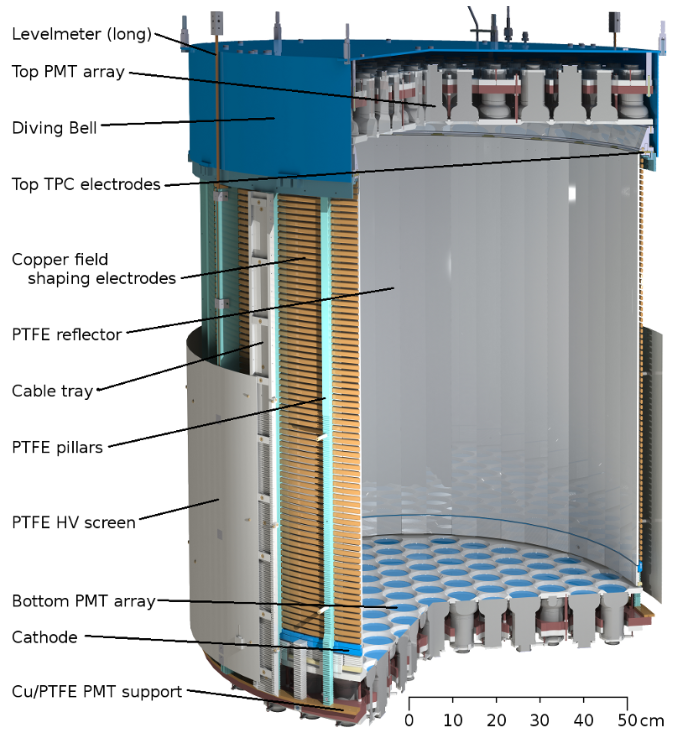
\includegraphics[width=0.8\textwidth]{XENON1TTPC}
\label{fig:xenon1t_tpc_tpc}
\end{figure}

There are five TPC electrodes that control the electric fields: the cathode, gate, anode, and top and bottom screening meshes.  They have
wired diameters of $\mathcal{O}(100)\ \mathrm{\mu m}$ and were designed to maximize S1 light collection.  The cathode is connected to a
PNC150000-1 NEG high voltage supply and pre-filling tests successfully reached voltages beyond -100 kV.  48
cm below the cathode is the bottom screening mesh (mentioned in \secref{subsec:xenon1t_pmts}).  The mesh is 12 mm above the bottom PMT
array and can be biased to reduce unwanted effects from the PMT and cathode E-fields.  The cathode and bottom screening mesh consist of
parallel wires and are gold-plated stainless steel, the latter of which increases the workfunction.  The gate rests just below the
liquid-gas interface and defines $z = 0$.  The anode is
situated 5 mm above the gate and is connected to a CAEN A1526P unit.  The fifth and final electrode is the top screening mesh 58 mm above
the anode and 11 mm below the top PMT array, and serves the same function is the same as the bottom mesh.  The top three electrodes are
made of stainless steel and are hex-etched.  Details for each electrode can be seen in \tabref{tab:xenon1t_tpc_electrodes} and
\figref{fig:xenon1t_tpc_efield} shows the simulated electric field for the settings during the first science run,Science Run 0.

\begin{table}
\centering
\begin{tabular}{cccccc}
\hline
Electrode & Type & Wire Diamater & Material & Transparency & Position \\
\hline
Top screening & hex meshed & $178\ \mathrm{\mu m}$ & stainless steel & 96.5\% & 63 mm \\
Anode & hex meshed & $178\ \mathrm{\mu m}$ & stainless steel & 89.8\% & 5 mm \\
Gate & hex meshed & $127\ \mathrm{\mu m}$ & stainless steel & 92.7\% & 0 mm \\
Cathode & parallel wires & $216\ \mathrm{\mu m}$ & gold-plated stainless steel & 97.2\% & -969 mm \\
Bottom screening & parallel wires & $216\ \mathrm{\mu m}$ & gold-plated stainless steel & 97.2\% & -1017 mm \\
\hline
\end{tabular}
\caption{Properties for TPC electrodes.  The cathode and bottom screening mesh have high transparency to optimize S1 light collection and
are gold-plated to increase workfunction.}
\label{tab:xenon1t_tpc_electrodes}
\end{table}

\begin{figure}
\centering
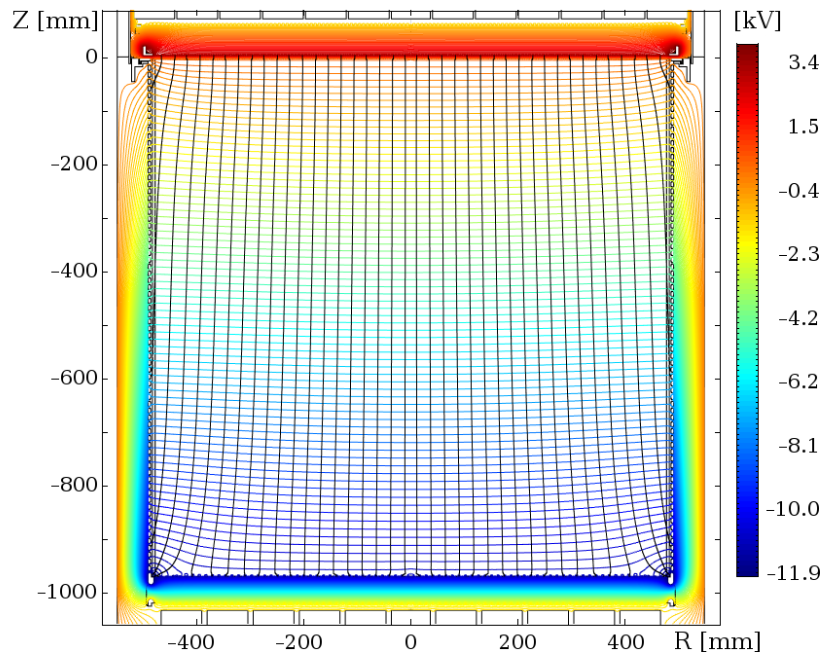
\includegraphics[width=0.8\textwidth]{ElectricField}
\caption{Finite element (COMSOL Multiphysics) simulation for E-field inside and around the TPC.  Field and equipotential lines are
shown.  The voltages for the cathode, gate, and anode are -12, 0, and 4 keV, respectively, or the settings for Science Run 0.  The field
is mostly uniform throughout the detector, minimizing possible biases that come from recombination, impurity attachment, etc.  Image
credit: \citeref{Aprile2017b}.}
\label{fig:xenon1t_tpc_efield}
\end{figure}

Four parallel-plate capacitors measure the liquid level.  They have a range of 10 mm with $30\ \mathrm{\mu s}$ precision and can be used
for observing tilts or raising (lowering) the TPC.  The liquid level's height is adjustable a gas-exhaust tube, and maintained with a
so-called ``diving bell" that uses controlled gas flow from purification to pressurize the GXe inside the TPC.  Two cylindrical levelmeters
with a range of 1360 mm extend from the bottom PMT array to above the diving bell and are used for filling and recovery.  Placed around the
field cage are cable trays that power and transfer signal from the PMTs.  They are made of PTFE and the cables are held
in place by PTFE spacers (\textbf{check if spacers is right word}).



\subsection{Cryogenics}
\label{subsec:xenon1t_cryo}
The TPC is stationed in the center of the water Cherenkov detector (\secref{subsec:xenon1t_water_shield}) and is encompassed by the inner
cryostat.  The cryostat
is stainless steel and electropolished to reduce radon emanation (\secref{}), since it is in direct contact with the xenon.  It is 1960 mm
tall by 1100 mm diamater and is metal-sealed
with Helicoflex.  Surrounding it is the 2490 mm tall by 1620 mm diamater outer cryostat.  It is also composed of stainless steel but
because there is no contact with xenon electropolishing is unncessary.  Materials were screened prior to construction for low-radioactivity
selection.  The two are thermally isolated by Torlon polyamide-imide spacers and
vacuum between them.  Heat loss is further mitigated to ${\sim} 75\ \mathrm{W}$ by aluminized mylar foil wrapped around the inner vessel.

A 10 m high stainless steel support structure was built inside the water tank.  Attached are three M20 rods that suspend the
cryostat.  They can be adjusted independently to tilt the cryostat, thereby changing the inclination of the LXe level with respect to the
TPC.  A chain secures the bottom of the outer vessel to the water tank floor to counteract buoyancy forces when the cryostat is empty.  A
double-walled pipe with inner and outer diameters 254 and 406 mm, respectively, connects with purification (\secref{subsec:xenon1t_pur}),
cooling,
pressurization for diving bell, and emergency recovery, and carries the PMT and auxiliary cables.  The voltage for the cathode is guided
in a separate pipe.  A schematic of the cryostat is shown

\begin{figure}
\centering
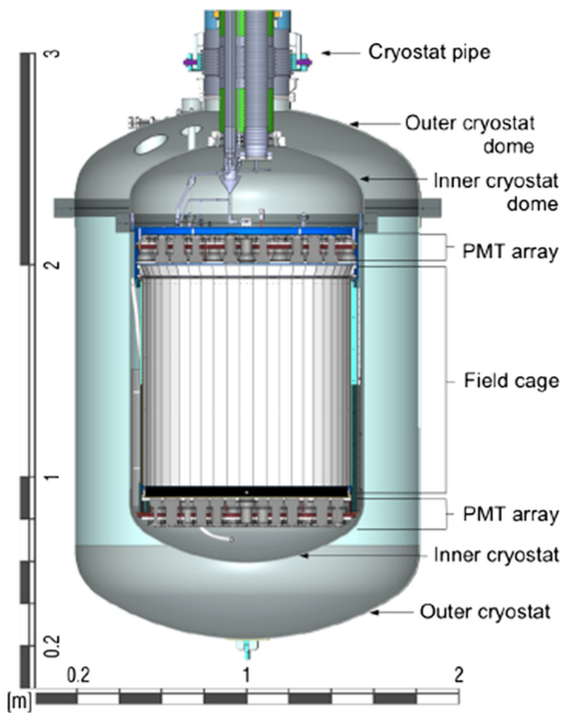
\includegraphics[width=0.8\textwidth]{CryostatDiagram}
\caption{Diagram of the cryostat.  Image credit: \citeref{Aprile2017c}.}
\label{fig:xenon1t_cryo_cryostat_diagram}
\end{figure}

A total of 3.5 tons of xenon is stored in the cryostat.  In addition to the 2.0 inside the TPC, the extra 1.5 is LXe between the
TPC and inner vessel or GXe above the liquid level.  The nominal LXe temperature is $T_{0} = -96^{\circ}\ \mathrm{C}$.  Gas near the top of
the cryostat is liquified by pulse-tube refrigerators (PTRs) into a funnel and flows back to the TPC through a designated pipe and
deposited in the inner vessel beneath the TPC.  Because
the PTRs are higher than the TPC the flow is guided by gravity.  \figref{fig:xenon1t_cryogenics_schmatic} shows the layout of the cryogenic
system.  The two PTRs occupy independent cooling towers and can each deliver ${\sim} 250\ \mathrm{W}$ of cooling power, and with
a total heat xenon heat load of ${\sim} 150\ \mathrm{W}$ only one needs to be active at any time.  The cooling towers along with much of the
GXe are located in the service building outside of the water tank  Each PTR connects to a copper cold finger
inside the inner cryostat so they can be removed without exposing the xenon to air.  A proportional-integral-derivative (PID) controller
monitors and adjusts the temperature of a resistive heater on the coldfinger to maintain stable pressure and temperature.

A third cooling tower uses liquid nitrogen ($\mathrm{LN_2}$) and is used in the case of an emergency if both PTRs are being serviced or the
heat load becomes too great from e.g. loss of power or insulation vacuum.  The $\mathrm{LN_2}$ flows from the $10 \mathrm{m^3}$ tank that
is used by ReStoX (\secref{subsec:xenon1t_restox}).  The cooling power can regulated by adjusting the $\mathrm{LN_2}$ evaporation rate.  In the event the PTRs
lose power the $\mathrm{LN_2}$ cooling tower must react immediately to prevent rising pressure that can be damaging to PMTs among other
things.  Sensors and controllers monitoring such a power loss are powered with uninterruptible power supplies (UPSs) to ensure a successful
transition and operation of $\mathrm{LN_2}$.

\begin{figure}
\centering
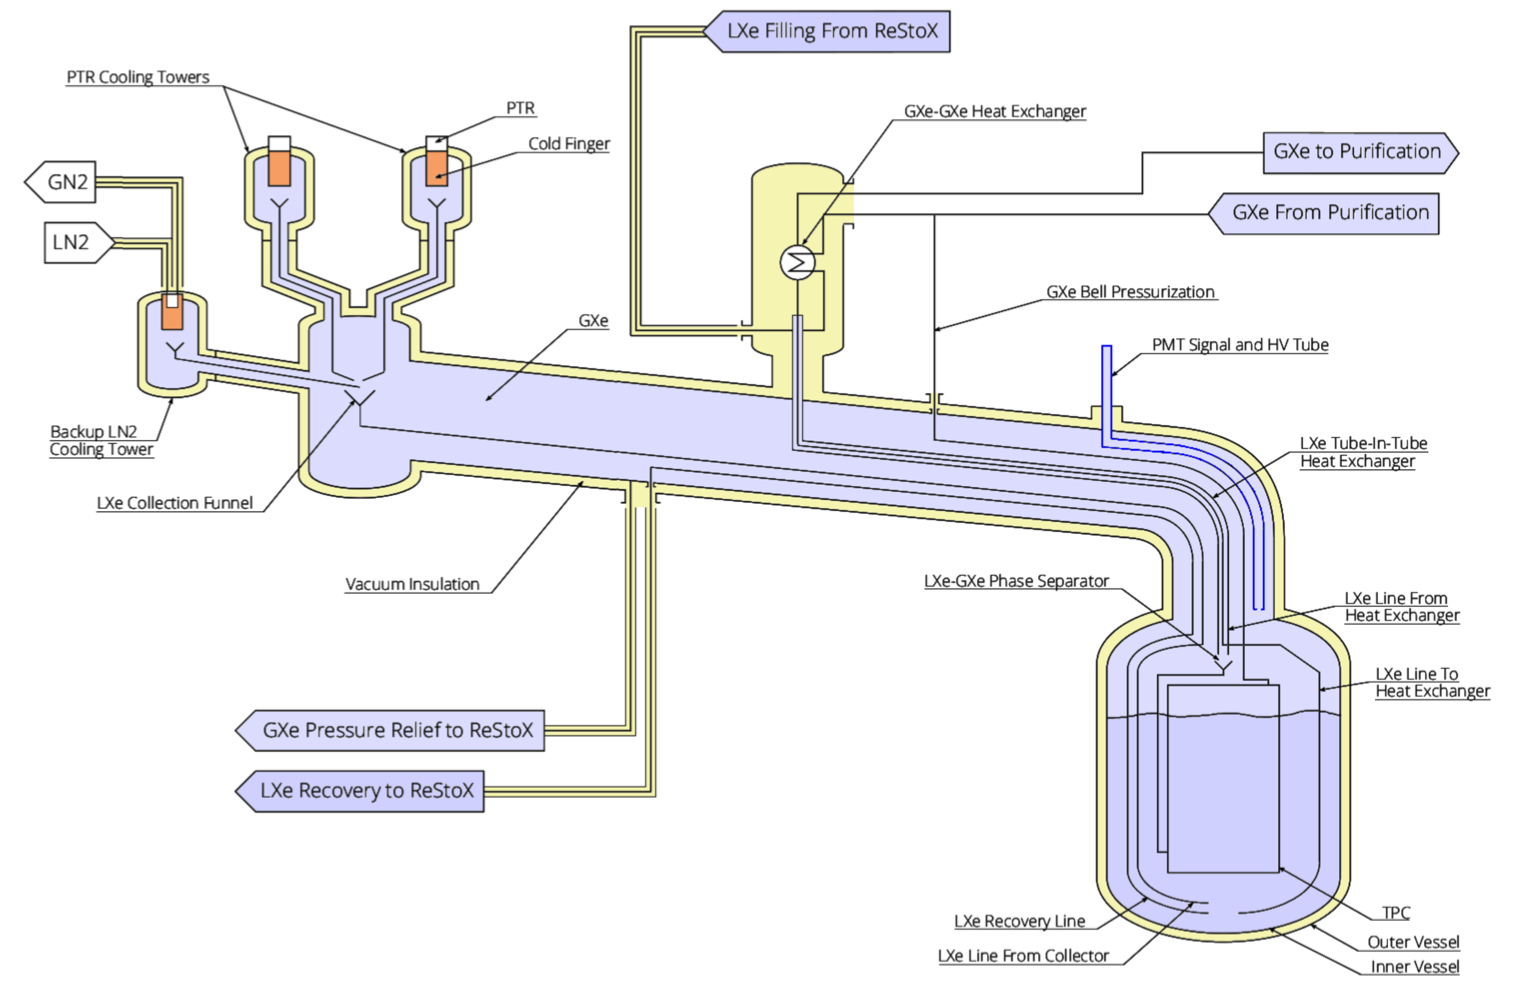
\includegraphics[width=\textwidth]{CryostatSchematic}
\caption{Layout of the cryogenic system.  Three cooling towers - two with PTRs and one backup $\mathrm{LN_2}$ - liquify GXe to return to
the TPC.  LXe is carried from the bottom of the cryostat to the purification system (\secref{subsec:xenon1t_pur}) through a heat exchanger
system, where
returning xenon is inserted into the bottom of the TPC with excess gas diffusing into the GXe.  A fraction of purified GXe is extracted
before the heat exchanger and used to maintain pressure inside the diving bell.  ReStoX (\secref{subsec:xenon1t_restox}) connections are
also shown.  Image credit: \citeref{Aprile2017b}.}
\label{fig:xenon1t_cryogenics_schematic}
\end{figure}

Connections to purification and ReStoX are shown in \figref{fig:xenon1t_cryogenics_schematic}.  The LXe carried to the purification system
passes through a heat exchanger system discussed in \secref{subsec:xenon1t_pur}.  This is not the case for recuperation since the xenon
does not need to be gaseous.

LXe from the beneath the TPC (near liquid line from PTRs) is removed for purification.  Once the xenon removed from the LXe it passes
through a two-phase heat exchanger system.  The function of the heat exchanger is for GXe (returning to the TPC) and LXe (leaving) to
exchange thermal energy.  This way the returning xenon is cooled before it reaches the TPC, and likewise removed xenon is heated before
the purification.  The first step of the system is the ``tube-in-tube" component where two concentric tubes carrying LXe (GXe) away from
(towards)
the TPC.  The second component is a plate heat exchanger and is closer to the purification system (i.e. returning xenon passes through
before tube-in-tube).

We can define the heat exchange
efficiency $\epsilon$ as the fraction of heat necessary for temperature change and vaporization that stays outside of the system.  A higher
efficiency results in greater thermal energy transferred between the GXe and LXe and thus decreases the heat load on the system.  This is
because instead of GXe entering the cryostat at roughly
room temperature, it returns at approximately that of LXe, with much of it having condensed to LXe, putting less stress on the
PTRs.  An essential ingredient of the heat transfer is the latent heat, which comprises ${\sim} 80\%$ of the total exchange.  The difference
in vaporization temperature of the outgoing xenon and condensation temperature of incoming xenon is given by

\begin{equation}
\Delta T_{\mathrm{ph}} = T_{\mathrm{gl}} (P_i) - T_{\mathrm{gl}} (P_o)
\label{eq:xenon1t_cryo_latent}
\end{equation}

where $T_{\mathrm{gl}} (P)$ is the temperature of the gas-liquid phase transition that depends on pressure, and $P_i$ and $P_o$ are the
pressures of the incoming and outgoing xenon, respectively.  Because the conditions of the dynamical gas flow
(\secref{subsec:xenon1t_pur}) cause $P_i > P_o$, $\Delta T_{\mathrm{ph}} > 0$, making it effective at heat transfer
(\citeref{Aprile2012b}).  A study with the Demonstrator - the
experiment used to for research and development for XENON1T - showed a heat exchange efficiency of
two heat exchangers in series of $\geq 96\%$ (\citeref{Aprile2012b}).  Following the parallel-plate exchanger a heater provides additional
thermal energy to the xenon moving towards the purification system.  The different systems that handle the xenon can be seen in
\figref{fig:xenon1t_cryo_overview}.

\begin{figure}
\centering
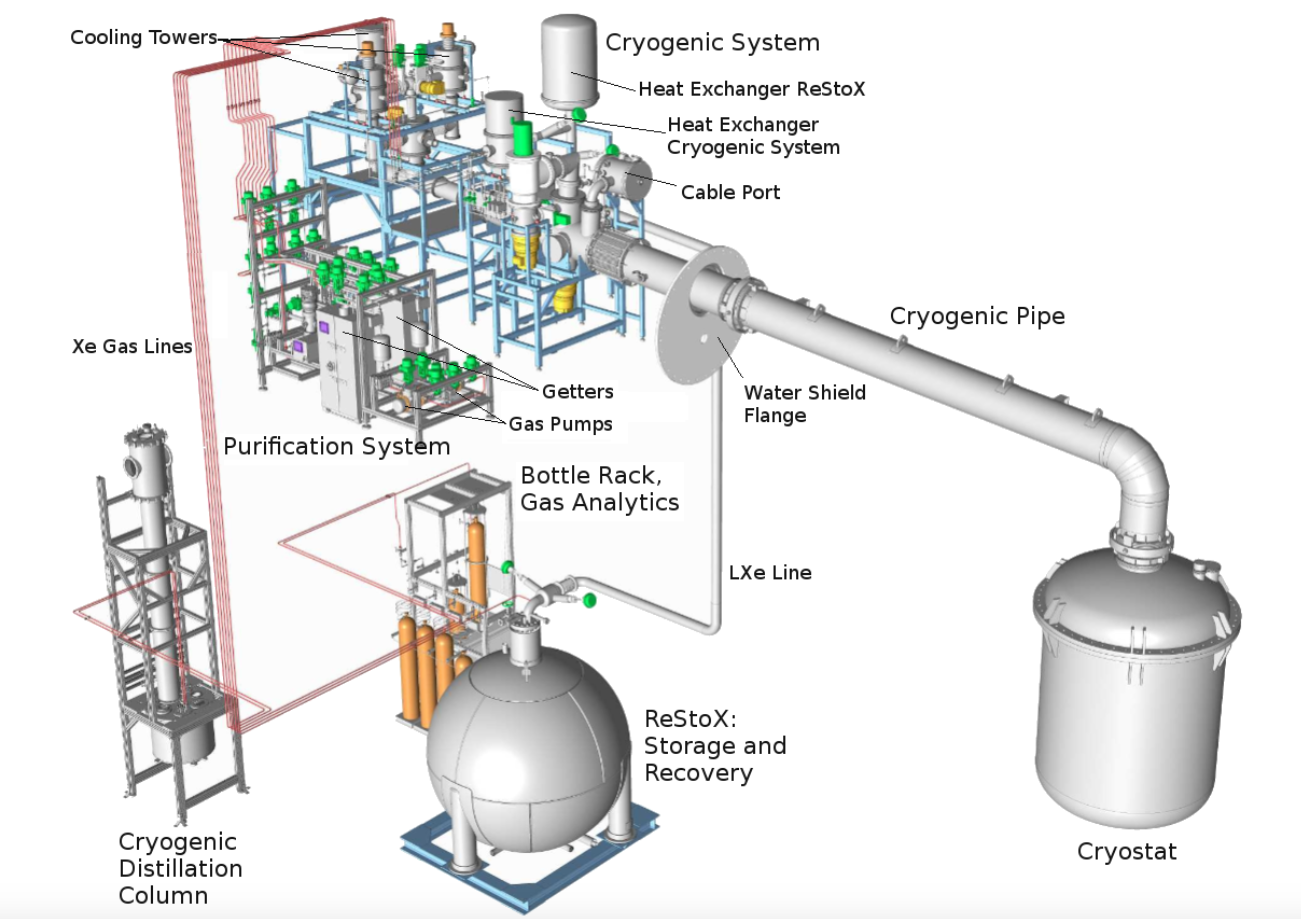
\includegraphics[width=\textwidth]{CryoOverview}
\caption{The various systems that handle xenon in the experiment: cryostat, cryogenics, purification, cryogenic distillation column,
ReStoX, bottle racks, and gas analytics station.  The water shield flange defines the region between the service building and the water
Cherenkov detector.  Image credit: \citeref{Aprile2017b}.}
\label{fig:xenon1t_cryo_overview}
\end{figure}



\subsection{Purification}
\label{subsec:xenon1t_pur}
Contamination in LXe can present a number of problems.  As mentioned in \secref{subsec:tpcs_working_principle} electronegative
impurities (e.g. O$_2$, H$_2$O, N$_2$O, etc.) will attach to drifting $e^-$, reducing the number that reach
the liquid surface and thus the S2.

Impurities will also attenuate scintillation, which pushes our energy threshold up as fainter signals become harder to detect.  This is
described by

\begin{equation}
I(x) = I_0 e^{-x / \lambda_{\mathrm{att}}}
\label{eq:xenon1t_pur_atten}
\end{equation}

where $I_0$ is initial number of photons, $I(x)$ is the number after traveling a distance $x$, and $\lambda_{\mathrm{att}}$ is the
attenuation length.  $\lambda_{\mathrm{att}}$ is dependent on the absorption and scatter lengths, $\lambda_{\mathrm{abs}}$ and
$\lambda_{\mathrm{scat}}$.  The absorption length describes the true loss of photons while the scatter refers to photons that elastically
scatter without energy loss.  The attenuation length can then be written
$1 / \lambda_{\mathrm{att}} = 1 / \lambda_{\mathrm{abs}} + 1 / \lambda_{\mathrm{scat}}$.  \figref{fig:xenon1t_pur_absorption_spectra} shows
the Xe scintillation spectrum along with the absorption coefficients for \otwo and \htwoo vapor at concentrations of 1 ppm.  We can see
there is large overlap at lower wavelengths - especially for H$_2$O - and that observations under these circumstances would lead to an
incorrect measurement of the scintillation spectrum.  In addition to electronegative there are intrinsic
impurities including Kr and Rn but these are discussed in \secref{subsec:xenon1t_kr_dist}.

\begin{figure}
\centering
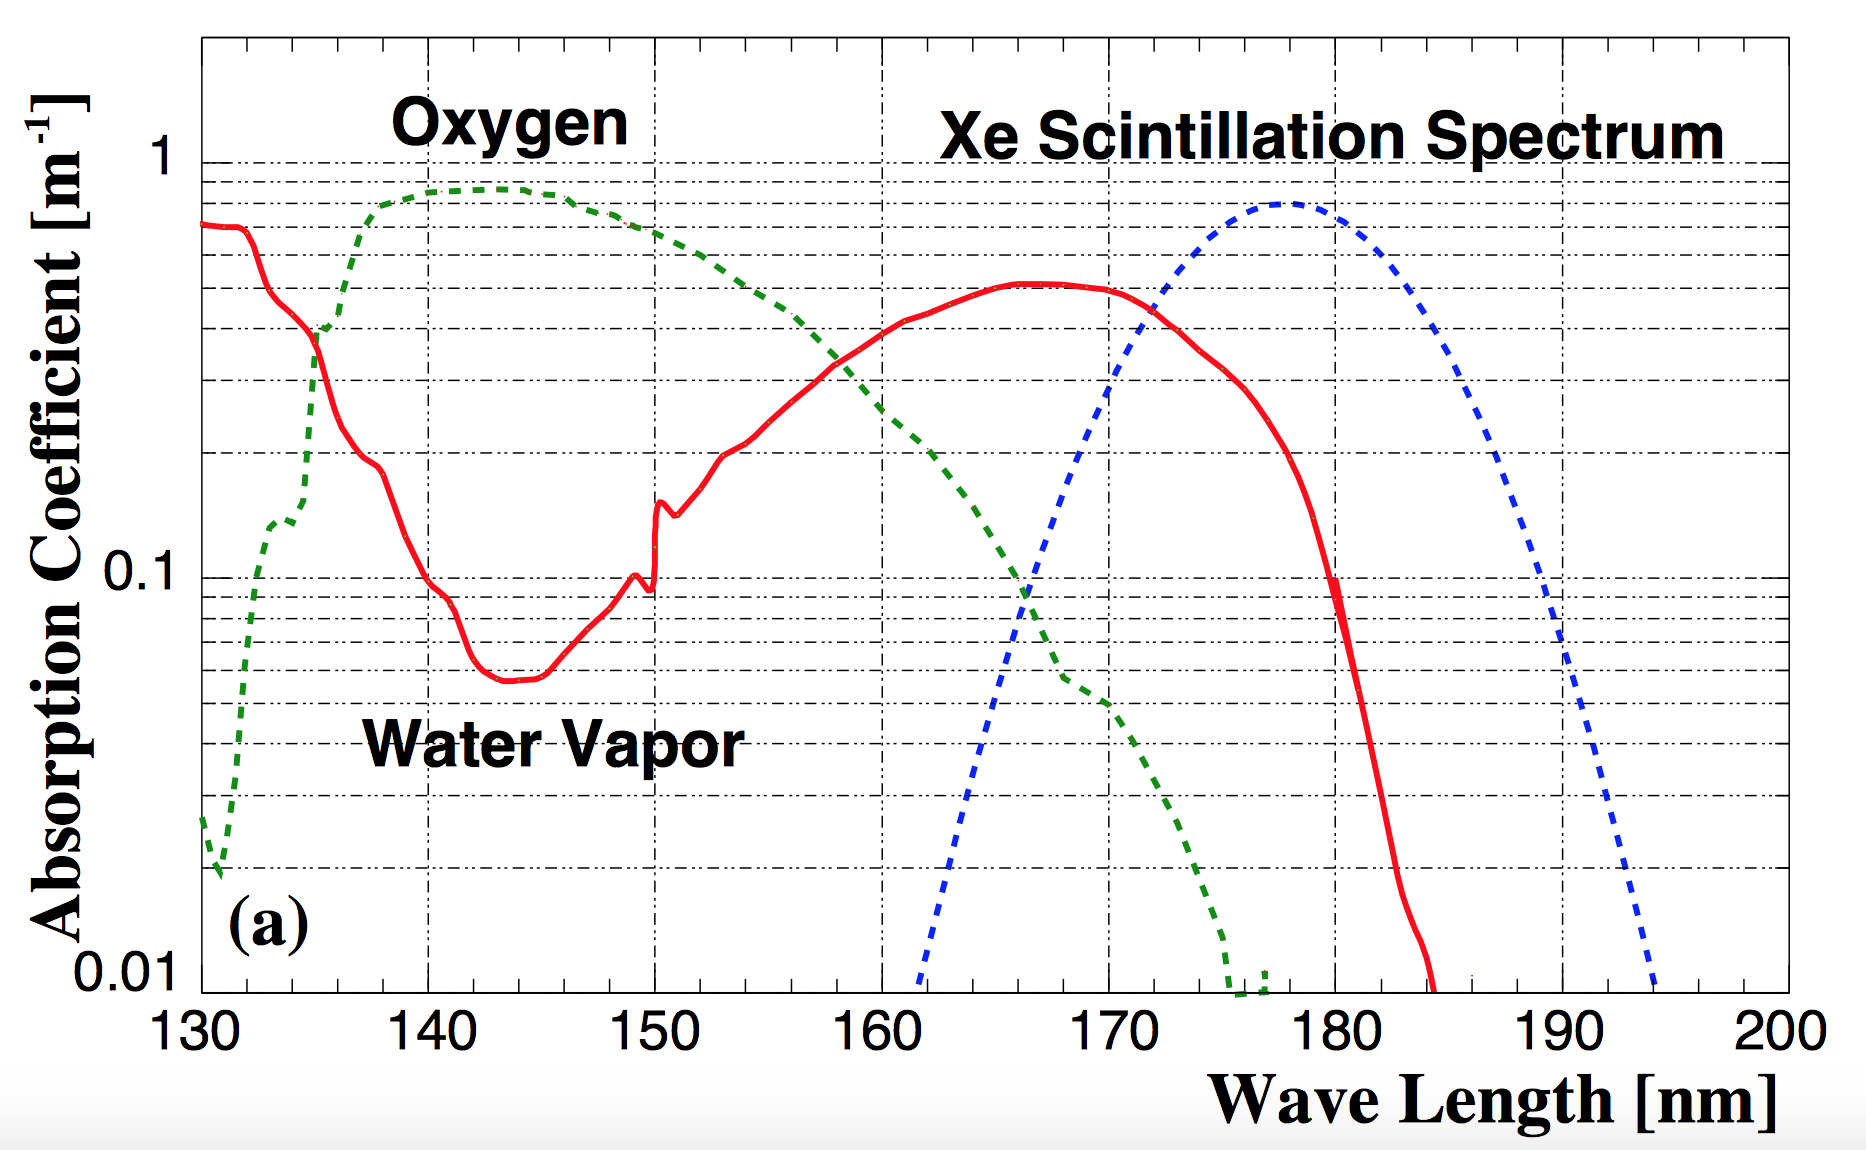
\includegraphics[width=0.8\textwidth]{AbsorptionSpectra}
\caption{Xe scintillation spectrum along with absorption coefficients for oxygen and water vapor present at 1 ppm.  \otwo has a maximum
value of overlap
with Xe of ${\sim} 0.1$ around 166 nm.  \htwoo covers a larger range of xenon's spectrum and has a much more significant impact, with a
maximum value of $> 0.4$ at approximately 172 nm and ${\sim} 0.2$ at 178 nm.  Image credit: \citeref{Ozone2005}.}
\label{fig:xenon1t_pur_absorption_spectra}
\end{figure}

\begin{figure}
\centering
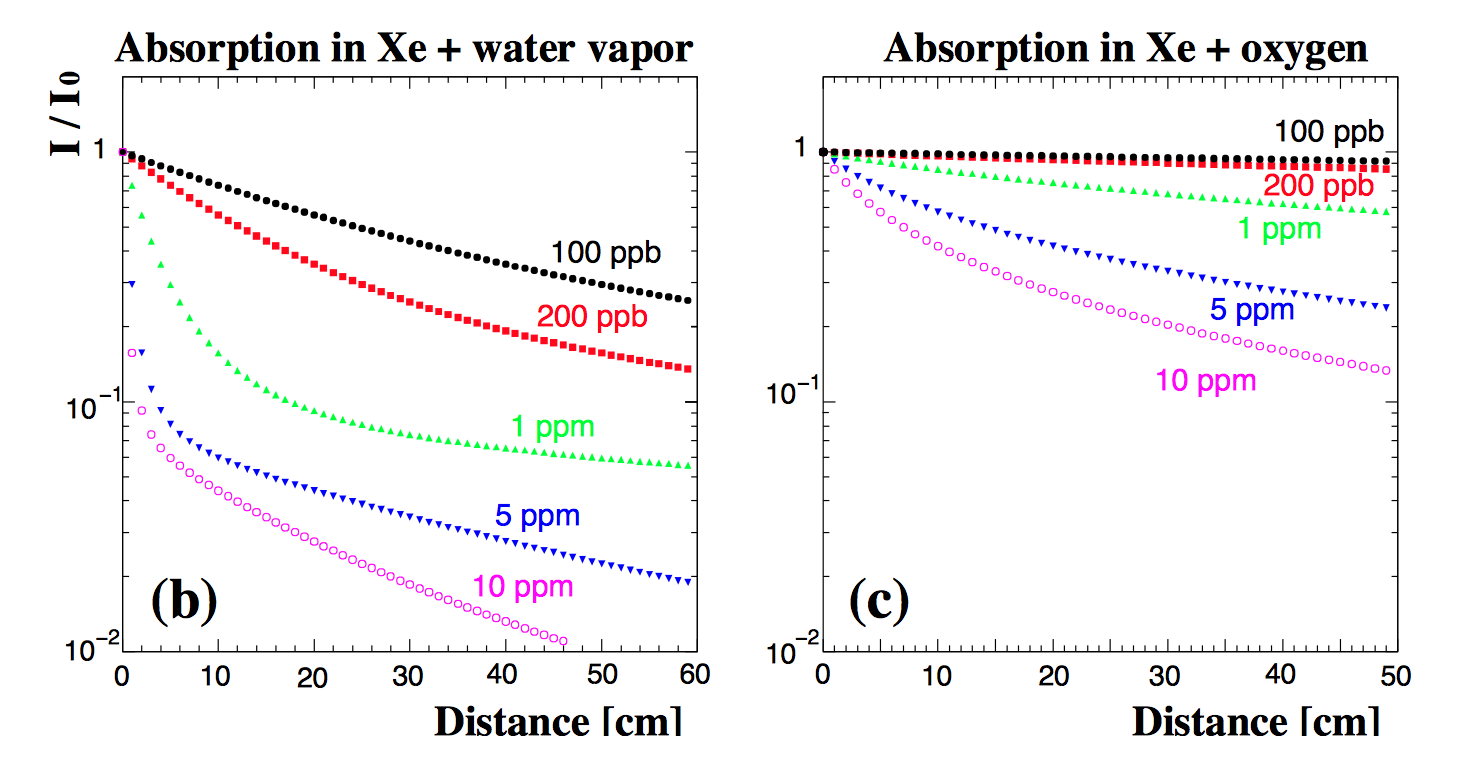
\includegraphics[width=\textwidth]{AbsorptionWithDistance}
\label{fig:xenon1t_pur_absorp_dist}
\end{figure}

Electronegative impurities come primarily from outgassing of detector materials.  They have different \electron attachment rates (see
\figref{fig:attachment_rate} for examples) so are measured in O$_2$-equivalent - that is, the analogous concentration of oxygen if it
were the only contaminant.  For LXe experiments the necessary concentration is $\mathcal{O}(10^{-9})$ parts per billion (ppb) or less.

In addition
to the GXe from the TPC (after passing through heat exchanger and heater as described in \secref{subsec:xenon1t_cryo}), connections are
made between
each of the cooling towers and the purification system.  Because impurities are lighter than xenon we can anticipate them having a larger
presence in the gas.  While the GXe impurity concentration has no direct effect on \electron loss, impurities should migrate between the
LXe and GXe.  Purifying the GXe then should largely reduce the impurities that pass into the liquid.

Xenon from ReStoX  (\secref{subsec:xenon1t_restox}) and bottles are also connected to the purification system.  A separate heat exchanger
sits between ReStoX and purification but is less effective when xenon is not incoming and outgoing (not during detector filling).  In
addition to cleaning the Xe as it is transfered to the from RestoX to the cryostat, the purification system connects ReStoX to the Kr
distillation column (\secref{subsec:xenon1t_kr_dist}).  The column returns the xenon after distillation to purification.  All systems that
feed into the purification system do so before the getters and are available as outputs as well.  A small tube between the purification
and cryostat before the heat exchanger siphons GXe to the TPC bell to maintain pressure, and is regulated by a flow controller.  The
numerous connections makes the purification system a hub for transferring xenon between systems.

\begin{figure}
\centering
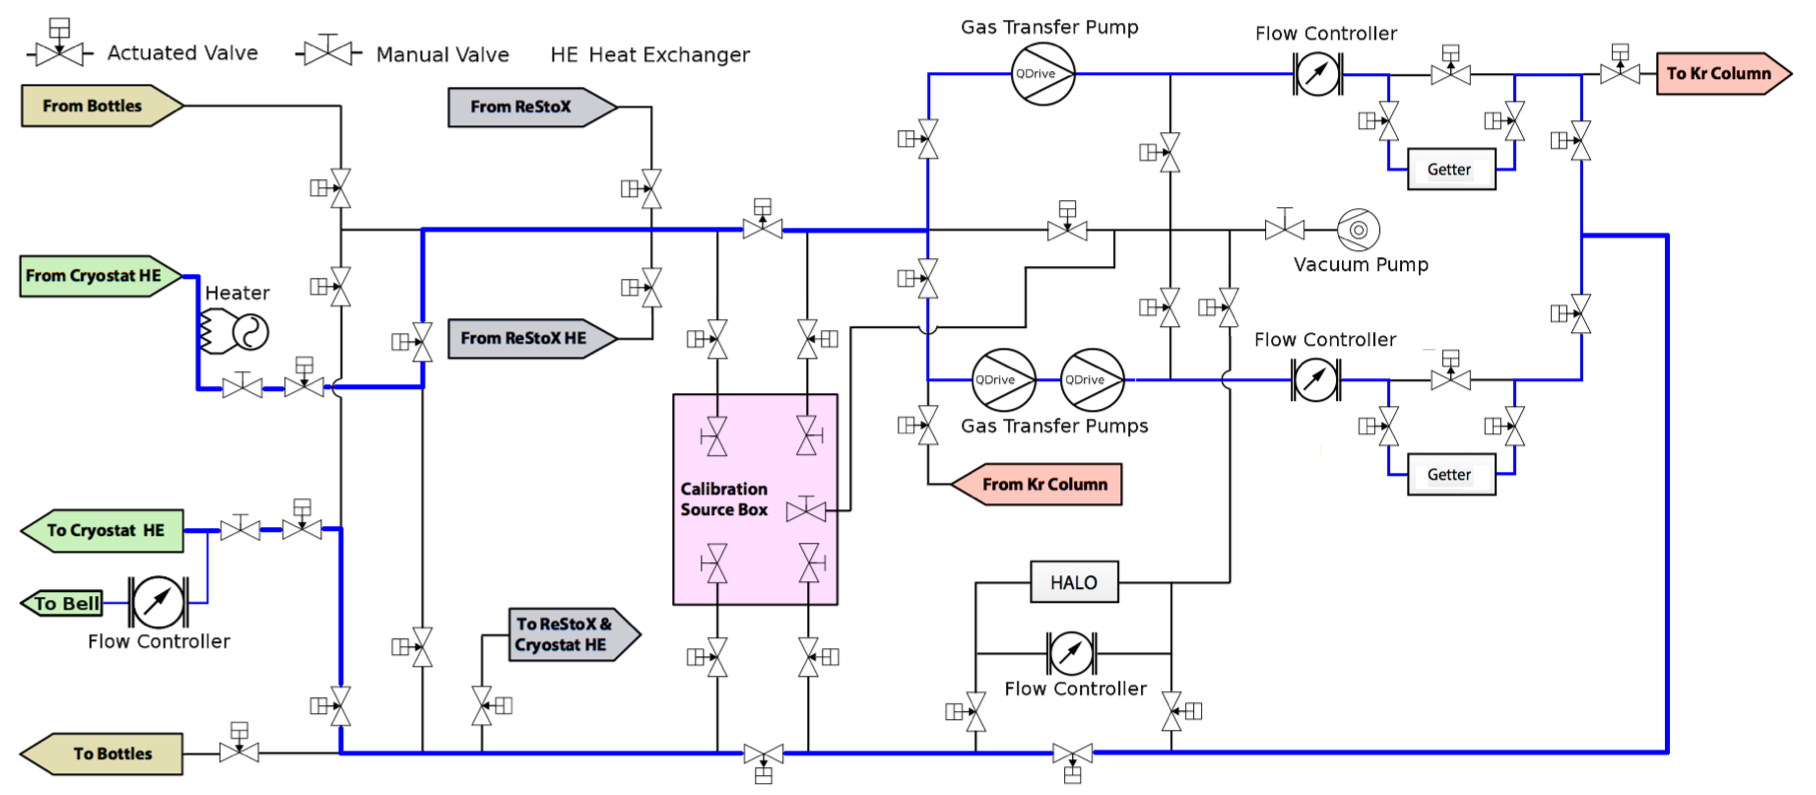
\includegraphics[width=\textwidth]{PurificationLayout}
\caption{Image credit: \citeref{Aprile2017b}.}
\label{fig:xenon1t_pur_schematic}
\end{figure}

The purification system consists of two redundant purification loops, each of which can operate independently of the other.  The flow
is driven by CHART QDrives, with one on one loop and two on the other.  They were chosen for their high-capacity and hermetically sealed
pump volume, the latter of which was not true with KNF pumps that were used in XENON100 (\textbf{check this}).  This is important because
exposure to air could cause a significant drop in purity, and has occurred in the past with KNFs.  They are
magnetically-resonant and operate via a compression space with oscillating externally-driven pistons.  Motors, valves, and pistons are
not lubricated, making it an excellent choice for high-purity.  Unfortunately QDrives emanate \ce{^{222}Rn} can require frequent
maintenance if operated at too great a voltage (for larger flow).  For the former \ce{Rn} emanation measurements were made prior to
installation with the lowest being chosen.  For the latter they are operated at safe conditions and since the beginning of Science Run 0
no issues have arisen.  It turns out the limiting factor on our circulation speed is not a result of the pumps but the pressure difference
from tubes leading to the system caused by too small a radius.  With the upgrade to XENONnT these will be replaced with larger-radii.  One
QDrive is installed in one loop and two in the other.

The flow of the GXe is maintained by two MKA 1579A mass-flow controllers - one on either branch.  The assumption before the experiment went
online was these would limit the speed when necessary, but because we did not achieve our goal these have minimal impact.  Still, they can
be used for further restriction.  The xenon then passes through SAES PS4-MT50-R high-temperature rare-gas purifiers, or getters.  They
use heated ($400^{\circ}\ \mathrm{C}$) zirconium to form unbreakable bonds with carbide, nitride, and oxide, lowering the impurity content
to < 1 ppb.  A bypass valve allows the xenon to pass un-purified in the event that the it does not need to be cleaned.

A Tiger Optics HALO+ H$_2$O monitor measures the water content in the purified GXe to track the purification efficiency.  It can measure
concentrations down to 400 ppt.  As with the getters, it can be bypassed.  The Xe is then forwarded to the cryostat, bell, ReStoX, or
bottles (Kr column occurs after the purification loops before the HALO).

The components of the system are electropolished and able to be baked up to ${\sim} 120^{\circ}\ \mathrm{C}$ for decreased outgassing during
operation.  The purification system has a number of valves that allow the versatility described in this section.  The majority are pneumatic and can
be operated remotely with the slow control system.  The remainder are manual valves situated in select locations: to and from the cryostat,
inside the calibration box, and before the vacuum pump, which can be used to evacuate individual sections or all of the system.  These are
in place as a precaution against accidental openings of the actuated valves that could produce problems.


\subsection{ReStoX}
\label{subsec:xenon1t_restox}
The Recovery and Storage system for XENON1T (ReStoX) hosts xenon not in use by other systems.  It is located roughly 7 on the ground floor of the
service building.  With a volume of 4.95 m$^{3}$
(diameter of 2.1 m), wall thickness of 28 mm, and ability to withstand pressures up to 73 bar, it can support as much as 7.6 tons of xenon
as a gas, liquid, or super-critical fluid.  It is constructed from stainless steel and insulated with vacuum from an outer sphere, where
thermal conductance is minimized with superinsulation and limited contact to an external heat load of ${\sim}50\ \mathrm{W}$.  To limit
impurity contamination while the Xe is in ReStoX the vessel and valves are metal sealed and electropolished.

The xenon is cooled by LN$_2$ that is housed in a 10 m$^3$ dewar adjacent to the service building.  This is done in part with 16 LN$_2$
lines that are welded to the inner vessel's outer surface.  To prevent over-cooling 16 stainless steel fins inside increase heat
exchanging.  A condenser and heater in the middle are used when the xenon is stored as a liquid, which is the nominal state of
operations.  The heater ensures solid xenon does not block pipes so Xe can transfer freely with other systems.  The total cooling power is
spread over 4.3 m$^2$ of copper with magnitude of over $>3\ \mathrm{kW}$.

\begin{figure}
\centering
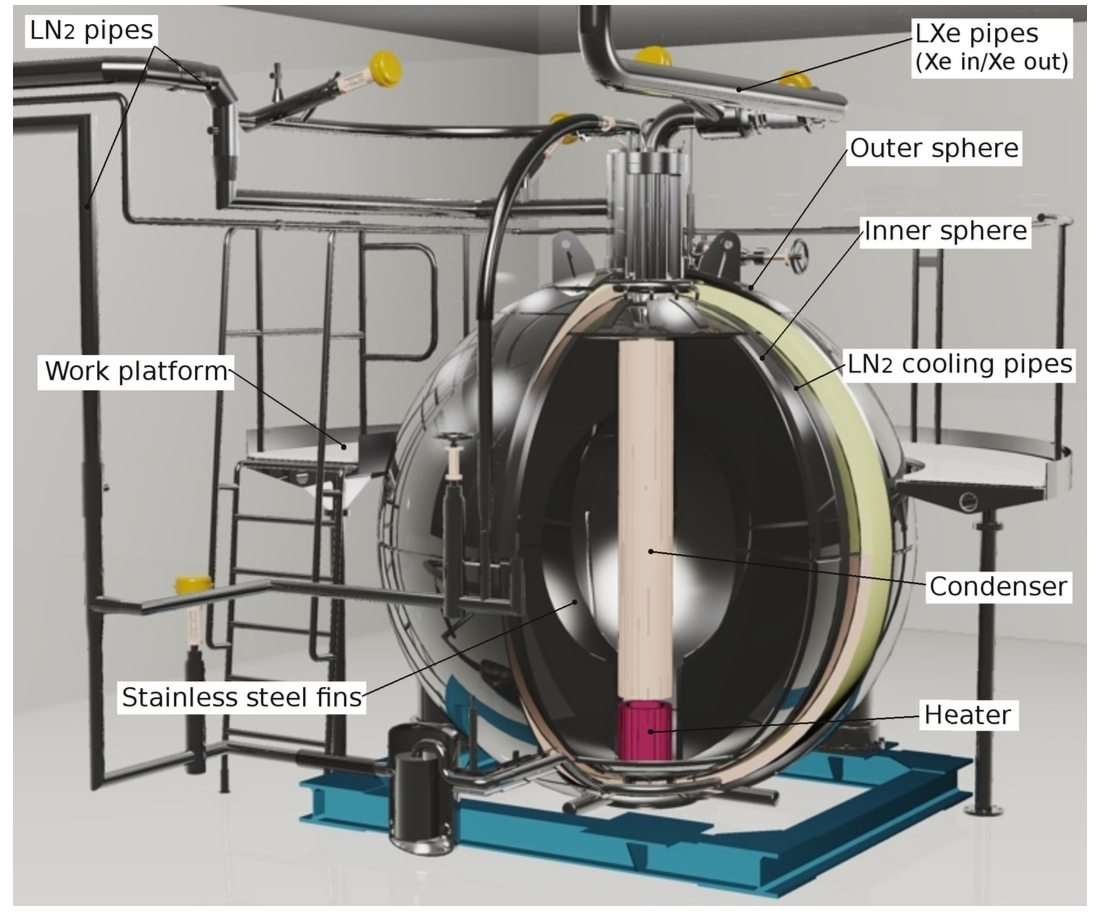
\includegraphics[width=0.8\textwidth]{ReStoX}
\caption{Image credit: \citeref{Aprile2017b}.}
\label{fig:xenon1t_restox_pic}
\end{figure}

Previous LXe experiments would fill the detectors by condensing the GXe from storage.  Similarly, recovery was done by allowing the LXe
in the cryostat to evaporate.  While this was achievable for detectors with $\mathcal{O}(100)\ mathrm{kg}$ of xenon, doing so
(\textbf{maybe it is just for filling, check}) for XENON1T would require approximately two months, and fast recovery in the event of an
emergency would not be possible.  This is solved through the purification system, which as mentioned in \secref{subsec:xenon1t_pur} can
pump xenon between systems (\textbf{check with someone about how xenon is recovered}).



\subsection{Krypton Distillation}
\label{subsec:xenon1t_kr_dist}
Commercial high-purity xenon generally has \ce{Kr} concentrations from 1 ppm down to 10 ppb.  This is not clean enough for LXe dark matter
detectors so additional distillation is necessary.  The reason for restricting the
krypton content is \ce{^{85}Kr}, which undergoes \betadecay with an end-point energy of 687 keV and a half-life of 10.76 years.  With
an expected fraction $\mathrm{^{85}Kr / ^{nat}Kr = 2 \times 10^{-11}}$ the required \ce{^{nat}Kr}/Xe concentration for its background to be
less than radon is $< 200\ \mathrm{ppq}$.  Details of the \ce{^{85}Kr} background can be found in \secref{sec:backgrounds}.

To achieve the intended purity we use a Kr distillation column, seen in \figref{fig:xenon1t_kr_dist_column}.  The column is has a total
height of 5.5 m and is kept in an insulation vessel at $10^{-5}\ \mathrm{mbar}$ to minimize thermal losses (citeref{Aprile2016b}).  GXe
that is passed to the column enters through a heat exchanger and is
liquified by the input condenser.  The input condenser uses a cryo-cooler (Leybold CP-50) at $-98^{\circ}\ \mathrm{C}$ and maximal power
of 100 W.  Next it passes to the package tube, built with 2.8 m of structured stainless steel package material (Sulzer EX) 45 cm in
diamater that has feeding ports for both liquid and gaseous xenon.  At the top of the tube is a second cryo-cooler (Leybold CP-140T)
operating at $-98^{\circ}\ \mathrm{C}$ with 200 W.  Liquified xenon will fall towards the bottom, where it is stored and heated by a
reboiler with a maximum of 300 W.  The Kr, with a lower atomic mass will drift towards the top of the column but will not liquify as its
boiling point is lower than $-98^{\circ}\ \mathrm{C}$.  Siphoning the xenon at the top then removes Kr at a much higher concentration than
present in the inlet GXe.  Purer Xe at the bottom is extracted where it passes through the heat exchanged before returning to the
purification system or ReStoX (\textbf{check this}).

\begin{figure}
\centering
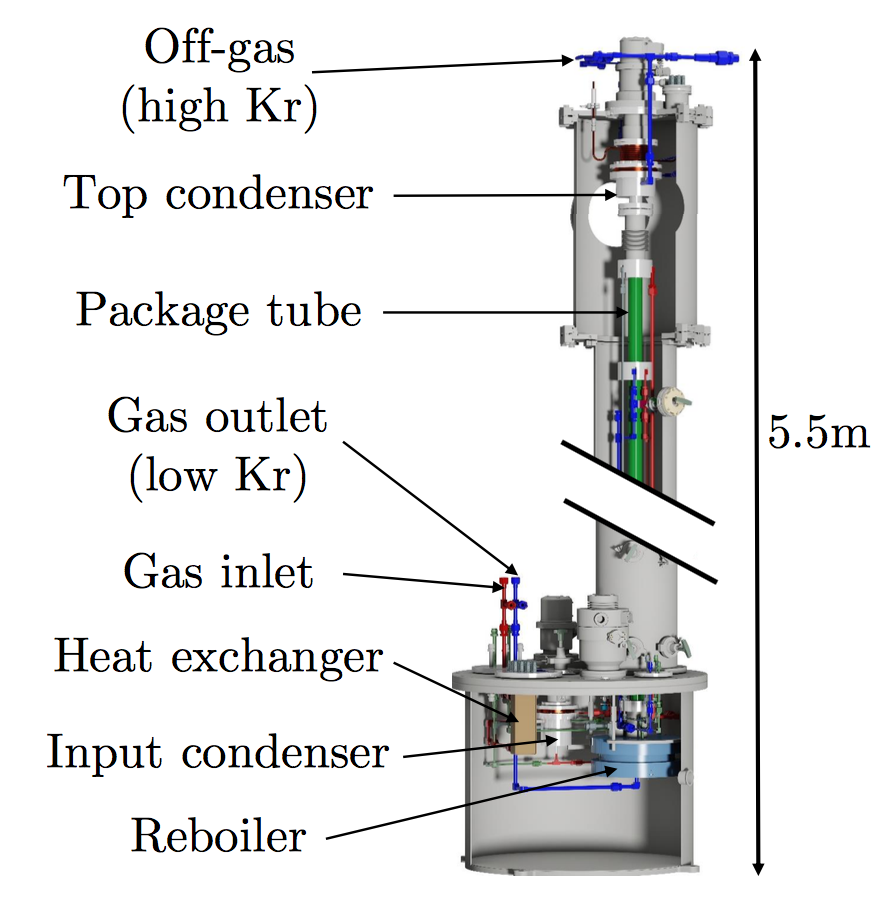
\includegraphics[width=0.6\textwidth]{KrColumn}
\caption{Image credit: \citeref{Aprile2017b}.}
\label{fig:xeno1t_kr_dist_column}
\end{figure}

After installed at LNGS the reduction of \ce{^{nat}Kr}/Xe was found to be $6.4_{-1.4}^{+1.9} \times 10^{5}$
(\citeref{Aprile2016b}).  Inlet flows have been shown to be stable up to 18 SLPM, but running all ReStoX xenon through distillation before
cryostat filling would take ${\sim}3$ weeks.  For this reason an ``online" removal system was used, where the xenon was distilled during
science run data taking.  Over 70 days 7\% of xenon passing through purification was diverted to the column and a total 0.07\% was
removed.  An initial \ce{^{nat}Kr}/Xe concentration of 60 ppb was decreased to $360 \pm 60\ \mathrm{ppq}$, the lowest ever realized in a
LXe dark matter experiment.  Such low concentrations are measured by a rare gas mass spectrometer (RGMS) that uses cryogenic gas
chromotography to separate the Kr from Xe, followed by a mass spectrometer for Kr measurement (\citeref{Lindemann2014}).

A second low-energy background comes from the \ce{^{222}Rn} decay chain.  While the distillation column was built and intended for Kr,
it was shown to work in a single stage distillation (\citeref{Bruenner2017}) and subsequently XENON100
(\citeref{Aprile2017d}).  It operates using the reverse principle, i.e. Rn-enriched xenon is coalesces near the bottom of the column.



\subsection{Water Shield}
\label{subsec:xenon1t_water_shield}
Limiting radiation from outside the experiment is essential to a dark matter search.  An active water Cherenkov detector encompasses the
cryostat, spanning 9.6 m in diamater and 10.2 m high.  It is filled with deionized water, which can fill the detector at up to
$2.2\ \mathrm{m^{3}/hour}$.  The tank shields the cryostat from neutrons and \gammarays that originate underground (from e.g. rocks),
decreasing the event rate by orders of magnitude.  It can identify muons as well as muon-induced neutrons by detecting showers initiating
outside the water tank.  If an event in the TPC coincides with one in the water tank it will usually be excluded incase the two are
related, acting as a muon veto.  The flux of muons at LNGS is $3.31 \pm 0.03 \times 10^{-8}\ \mathrm{cm^2\ s^{-1}}$ with average energy
${\sim}270\ \mathrm{GeV}$ (\citeref{Aprile2017b}).  The flux of muons for various underground laboratories is shown in
\figref{fig:xenon2t_water_shield_flux}.

\begin{figure}
\centering
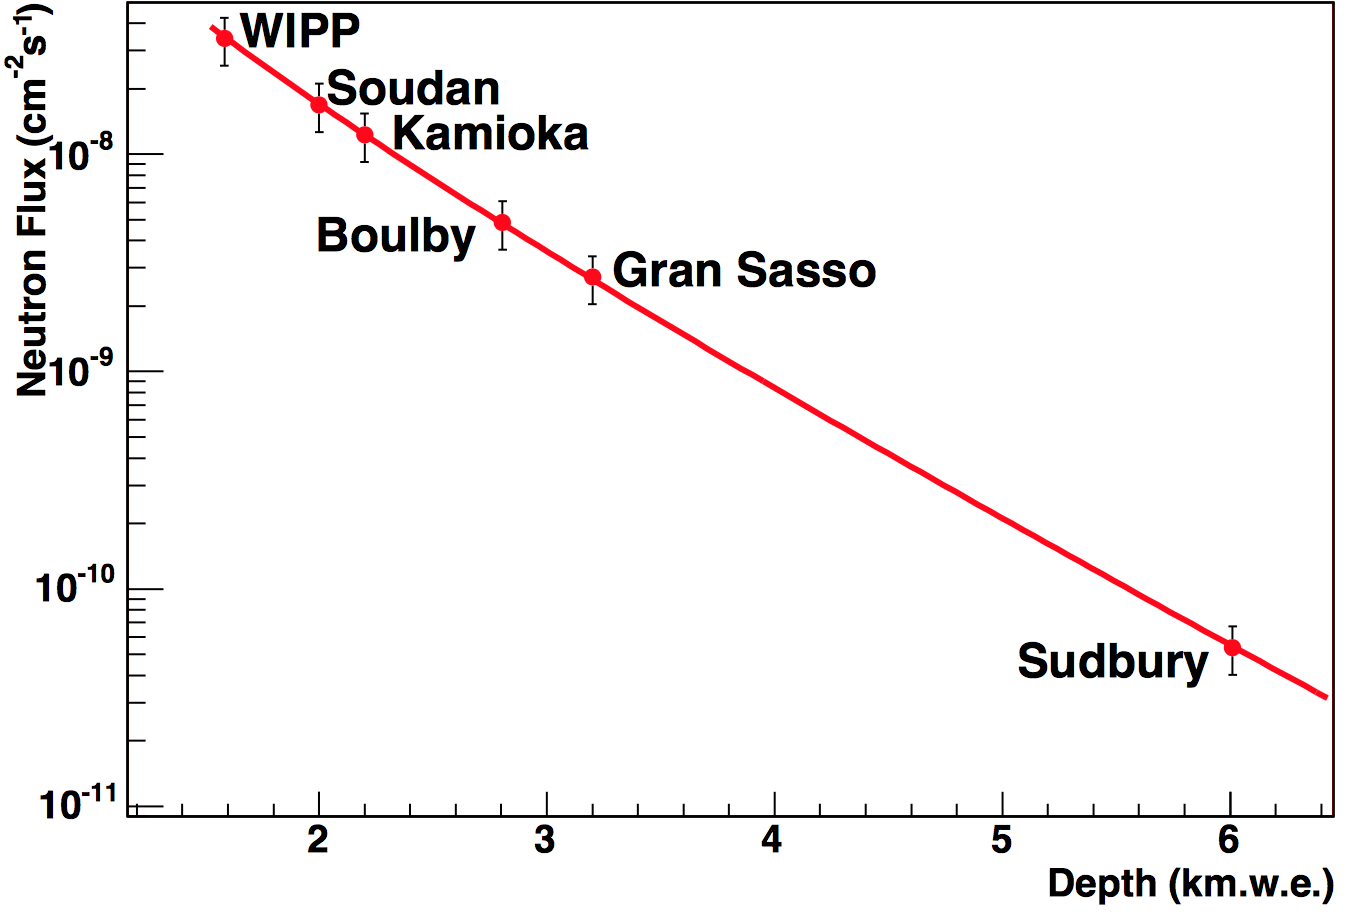
\includegraphics[width=0.8\textwidth]{MuonFluxOverDepth}
\caption{Image credit: \citeref{Mei2006}.}
\label{fig:xenon1t_water_shield_flux}
\end{figure}

84 Hamamatsu R5912ASSY PMTs are placed in five rings along the inner wall of the tank, each 2.5 m apart in height.  The lowest
($z = 0\ \mathrm{m}$) and highest ($z = 10\ \mathrm{m}$) each contain 24, while the three between them have 12.  The quantum efficiency
is ${\sim}30\%$ between 300-600 nm.  To increase the chance of photon detection the inner wall is coated with foil (3M DF2000MA) that has
nearly 100\% reflectivity at $> 400\ \mathrm{nm}$, (\citeref{2017Geis}).  However, ${\sim}90\%$ of light is absorbed for $<370 \mathrm{nm}$
and 3-7.5\% from $250 < \geq \lambda \geq 370\ \mathrm{nm}$ is wavelength shifted to more favorable values for the PMTs.

\begin{figure}
\centering
\includegraphics[width=\textwidth]{MuonVetoPhoto}
\label{fig:xenon1t_water_shield_photo}
\end{figure}

\begin{figure}
\centering
\includegraphics[width=\textwidth]{InsideWaterTank}
\label{fig:xenon1t_water_shield_interior}
\end{figure}



\subsection{Calibrations}
\label{subsec:xenon1t_calibrations}
Calibrations are used for a host of purposes including understanding energy resolution, light collection efficiency, electron lifetime,
$g1$, $g2$, electronic and nuclear recoil bands, and many more.  Depending on the source they can be performed inside the TPC (internal) or
outside (external).  Here I cover the different calibrations and the purposes they serve; additional details and results are in
\secref{sec:det_char}.


\subsubsection{Internal}
\label{subsubsec:xenon1t_calibrations_internal}
Internal calibrations allow us to describe how our detector observes events throughout the entire TPC.  This is preferabel to external
calibrations, where only part is used.  The calibration source box is installed in the purification system (pink region in
\figref{fig:xenon1t_pur_schematic}) and contains valves opening to the GXe both before and after the getters.  When the valves are opened,
the source will flow into the GXe stream and into the cryostat and mix with the xenon.  We therefore only use sources that do not introduce
electronegative impurities.  The source will quickly spread itself throughout the entirety of the xenon, giving a uniform distribution,
and allowing us to improve our understanding of how variation in observables relates to position.

\kryptonmeta has two monoenergetic decays at 32.15 ($t_{1/2} = 1.83\ \mathrm{h}$) and 9.4 keV ($t_{1/2} = 154.4\ \mathrm{ns}$).  The short
half-lives coupled with its final decay product, \ce{^{83}Kr} being stable makes it a great choice to calibrate the light collection
efficiency (LCE) and measure the electron lifetime.

\radoncal is used to calibrate the ER band as \ce{^{212}Pb} - one of its daughters, is a $\beta$-emitter with endpoint energy
569.91 keV.  There are additional $\alpha$, $\beta$, and $\gamma$ emissions throughout the chain that can be used for additional studies,
including measuring the electron lifetime with the \ce{^{212}Bi} $\alpha$-decay (6.207 MeV).  The longest half-life in the chain is
\ce{^{212}Pb} with $t_{1/2} = 10.6\ \mathrm{h}$ (next longest is \ce{^{212}Bi} with $t_{1/2} = 1.00\ \mathrm{h}$), which allows DM data
to resume within several days.

Tritiated methane (CH$_{3}$T) is a very attractive candidate because of it's low-energy $\beta$-emission.  With a 18.6 keV endpoint energy,
it is an ideal candidate for calibrating the low-energy (cs1 < 100 pe, \textbf{check this}) ER band, and even measuring the light and
charge yield in a relatively unexplored but important
region.  This was originally done by LUX (\citeref{LUX2016}) and subsequently performed with XENON100 (\citeref{Aprile2017e}).  However,
with a half-life of $t_{1/2} = 12.3\ \mathrm{y}$ it must be removed completely by the getters to avoid introducing a new background.  This
is further complicated by a suspicion that the methane adheres to the cryostat, prohibiting total removal.  For this reason a CH$_3$T
calibration has not yet been conducted in XENON1T.

PMT gains are calibrated using blue LEDs at low light levels.  Unlike the previous sources this calibration is done using cables that are
carried from the data acquisition (\secref{subsec:xenon1t_daq}) into the TPC.  They are fixed at various heights and angles and flash
at periodic intervals.  The result is an SPE spectrum as shown in \figref{fig:xenon1t_pmt_spe}.

\begin{figure}
\centering
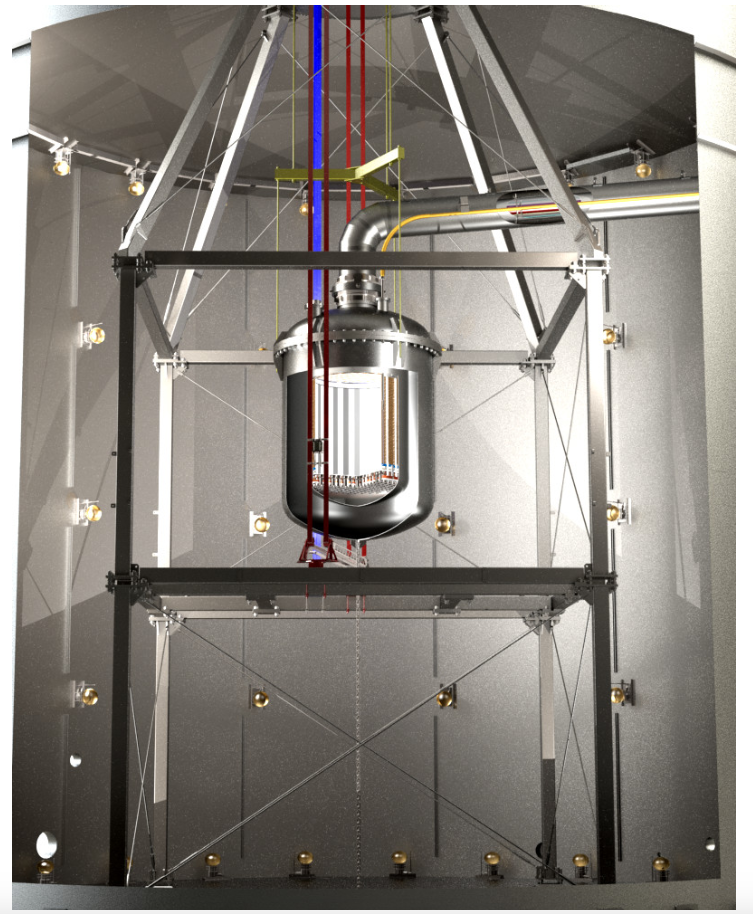
\includegraphics[width=\textwidth]{WaterTankInside}
\label{fig:water_tank_inside}
\end{figure}



\subsubsection{External}
\label{subsubsec:xenon1t_calibrations_external}
External calibrations are performed with a source outside the cryostat.  In XENON100 this was done by inserting a source inside the lead
shielding; however, the water tank in XENON1T makes this a more complicated task.  The resolution was the installation of two ``I-belts"
along the height of the detector and one ``U-belt" that also extends underneath, as shown in \figref{fig:xenon1t_calibration_belts}.  These
allow the sources to be lowered from the roof of the tank, as well as calibrate from different locations, so long as they are on the
belts.  They are removed during dark matter data taking.

\begin{figure}
\centering
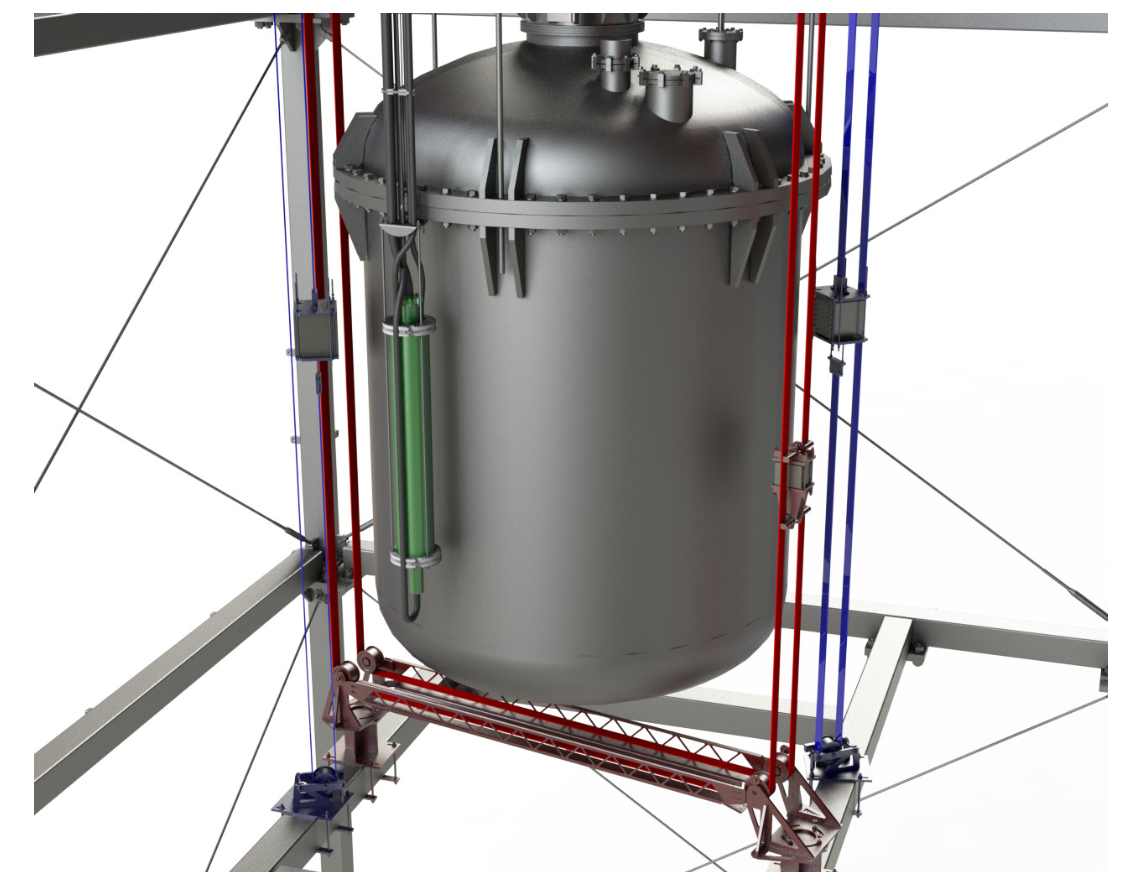
\includegraphics[width=0.8\textwidth]{TPCCalibrations}
\caption{Image credit: \citeref{Aprile2017b}.}
\label{fig:xenon1t_calibrations_belts}
\end{figure}

External $\gamma$ sources include \ce{^{137}Cs}, with an energy of 661.7 keV, and \ce{^{228}Th}, with a number of energies between 511 keV
and 2.614 MeV.  These are installed in W-collimators that restrict the \gammarays to a cone of $40^{\circ}$.  Additionally, \ce{^{60}Co}
in the cryostat flanges with 1.173 and 1.333 MeV lines can also be used.

Nuclear recoil sources \ambe and a deuterium-deuterium (DD) neutron generator (NG) are also done outside the TPC.  It is also deployed in a
W-collimator and emits MeV neutrons.  Details are discussed in \secref{subsubsec:er_nr_calibrations_parameter_determ_nr}.



\subsection{Data Acquisition}
\label{sec:xenon1t_daq}
The data acquisition (DAQ) is on the second floor of the service building.

\begin{figure}
\centering
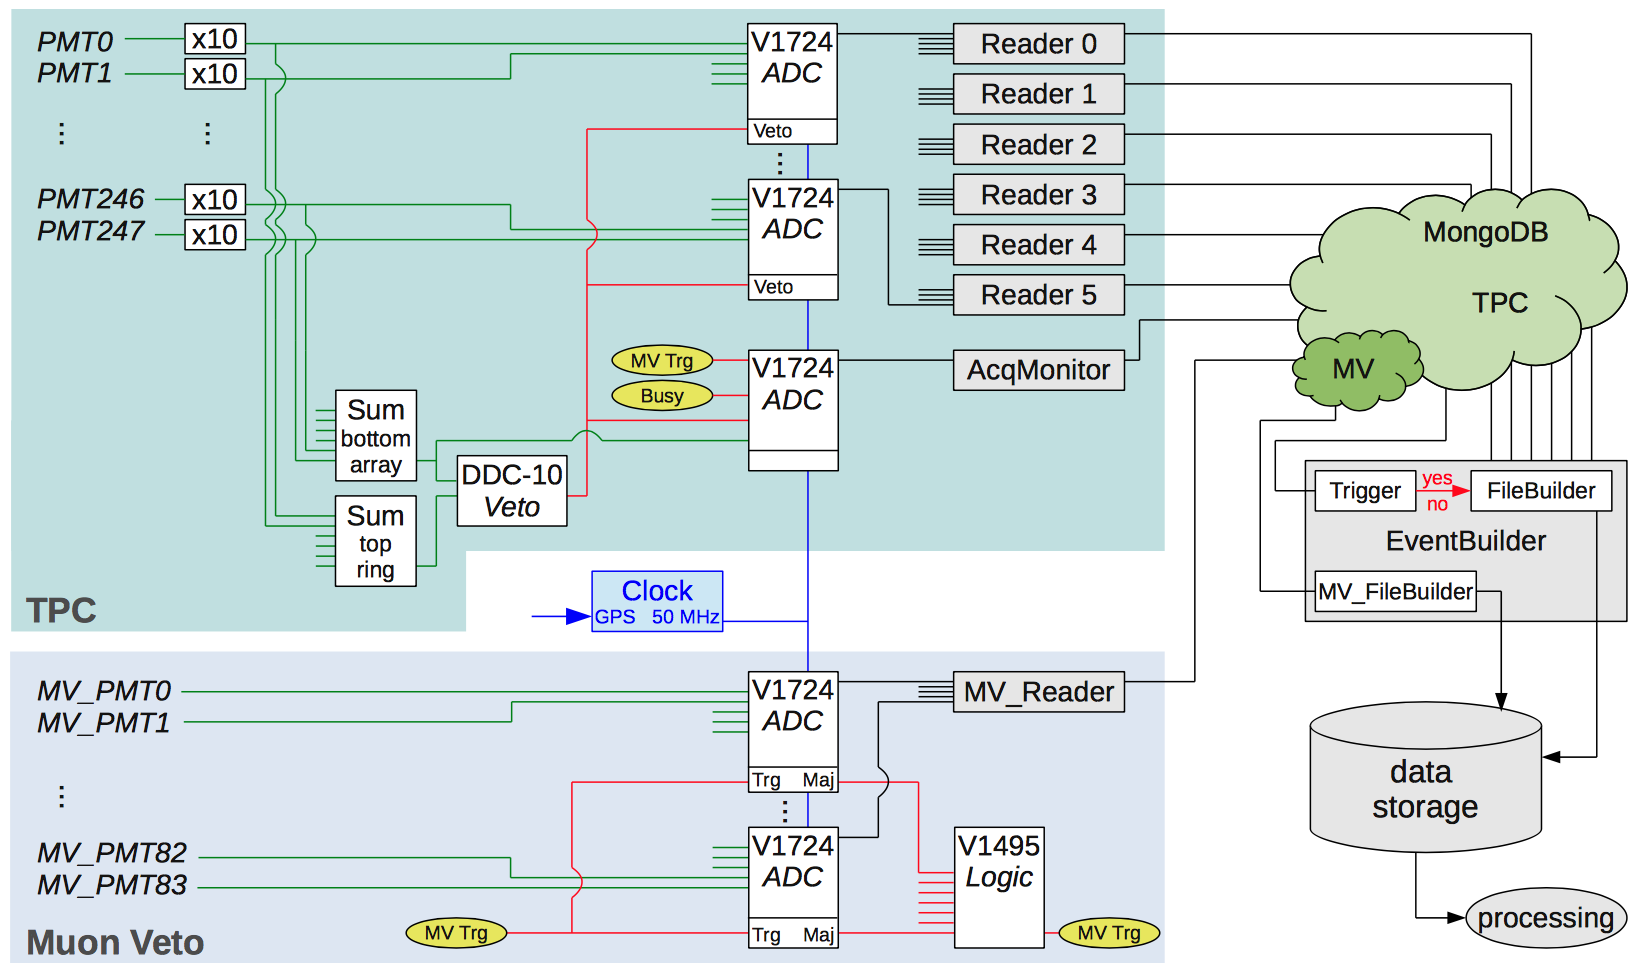
\includegraphics[width=\textwidth]{DAQ}
\label{fig:xenon1t_daq_schematic}
\end{figure}

\begin{figure}
\centering
\includegraphics[width=\textwidth]{Panoramic}
\label{fig:xenon1t_panoramic}
\end{figure}



\section{Backgrounds}
\label{sec:backgrounds}
To reach the desired sensitivity it is crucial to lower our backgrounds as much as possible, and just as importantly, understand
them.  Our backgrounds mainly come from the detector materials, radioactive isotopes distributed inside the xenon, and space.

\subsection{Detector Materials}
\label{subsec:backgrounds_detector_materials}
As mentioned in \secref{subsec:xenon1t_pmts} and \secref{subsec:xenon1t_cryo} detector materials were screened before purchasing to ensure
those with the lowest radioactivity were chosen.  The high self-shielding power of LXe prevents the radiation from penetrating far into
the detector, stopping the majority within several cm.  Still, it is important to understand our background for a number of reasons.  The
first is we want to maximize our FV.  But because including these events can have a negative effect on our sensitivity, we need to know
what a safe distance from the top, bottom, and wall are.  The second is once we choose our FV it is important to have a reliable estimate
of the number of events that will ``leak" into our FV, known as ``leakage events".  Failing to have an accurate prediction can result in
a cost in sensitivity.  A third reason is these events can play a significant role in characterizing the detector.

The primary isotopes from materials that play a role in our background are \ce{^{40}K}, \ce{^{60}Co}, \ce{^{235}U}, and the decay chains
of and \ce{^{238}U}, \ce{^{232}Th}, \ce{^{228}Th}, and \ce{^{226}Ra}.  In fact, although \ce{^{226}Ra} and \ce{^{228}Th} are part of the
\ce{^{238}U} and \ce{^{232}Th} chains, respectively, the measured disequilibrium prompts us to separate them as
$\mathrm{^{238}U} \rightarrow \mathrm{^{230}Th}$ and $\mathrm{^{226}Ra} \rightarrow \mathrm{^{206}Pb}$ for \ce{^{238}U}, and
$\mathrm{^{232}Th} \rightarrow \mathrm{^{228}Ac}$ and $\mathrm{^{228}Th} \rightarrow \mathrm{^{208}Pb}$ for \ce{^{232}Th}.  The full
\ce{^{238}U} and \ce{^{232}Th} chains can be seen in \figref{fig:backgrounds_decay_chains}.

An important realization came from tracking the number of \ce{^{222}Rn} and \ce{^{218}Po} $\alpha$-decays.  By monitoring the
decays within a radius $r$ we discovered that the rate was increasing with time.  However, if we did not apply a radial cut the decay rate
was constant.  This could be explained by charge accumulation on the wall of the TPC - primarily by wall events.  This turned out to be an
important consideration as over the course of dark matter data taking the number of events within a fixed FV would be expected to
grow.  The measured increase for \ce{^{222}Rn} and \ce{^{218}Po} is shown in \figref{fig:backgrounds_wall_charge}.


At $E \gtrsim 500\ \mathrm{keV}$ the background contribution becomes dominated by the detector materials, except for
${\sim} 1400-2100\ \mathrm{keV}$ where \ce{^{136}Xe} is slightly larger.  For the energy region for spin-independent WIMP dark matter
though it is outpaced by more than an order of magnitude inside a 1-ton FV.  \figref{fig:backgrounds_er_spectrum} shows the predicted ER
backgrounds using Monte Carlo.

\begin{figure}
    \centering
    \begin{subfigure}[t]{0.5\textwidth}
        \centering
        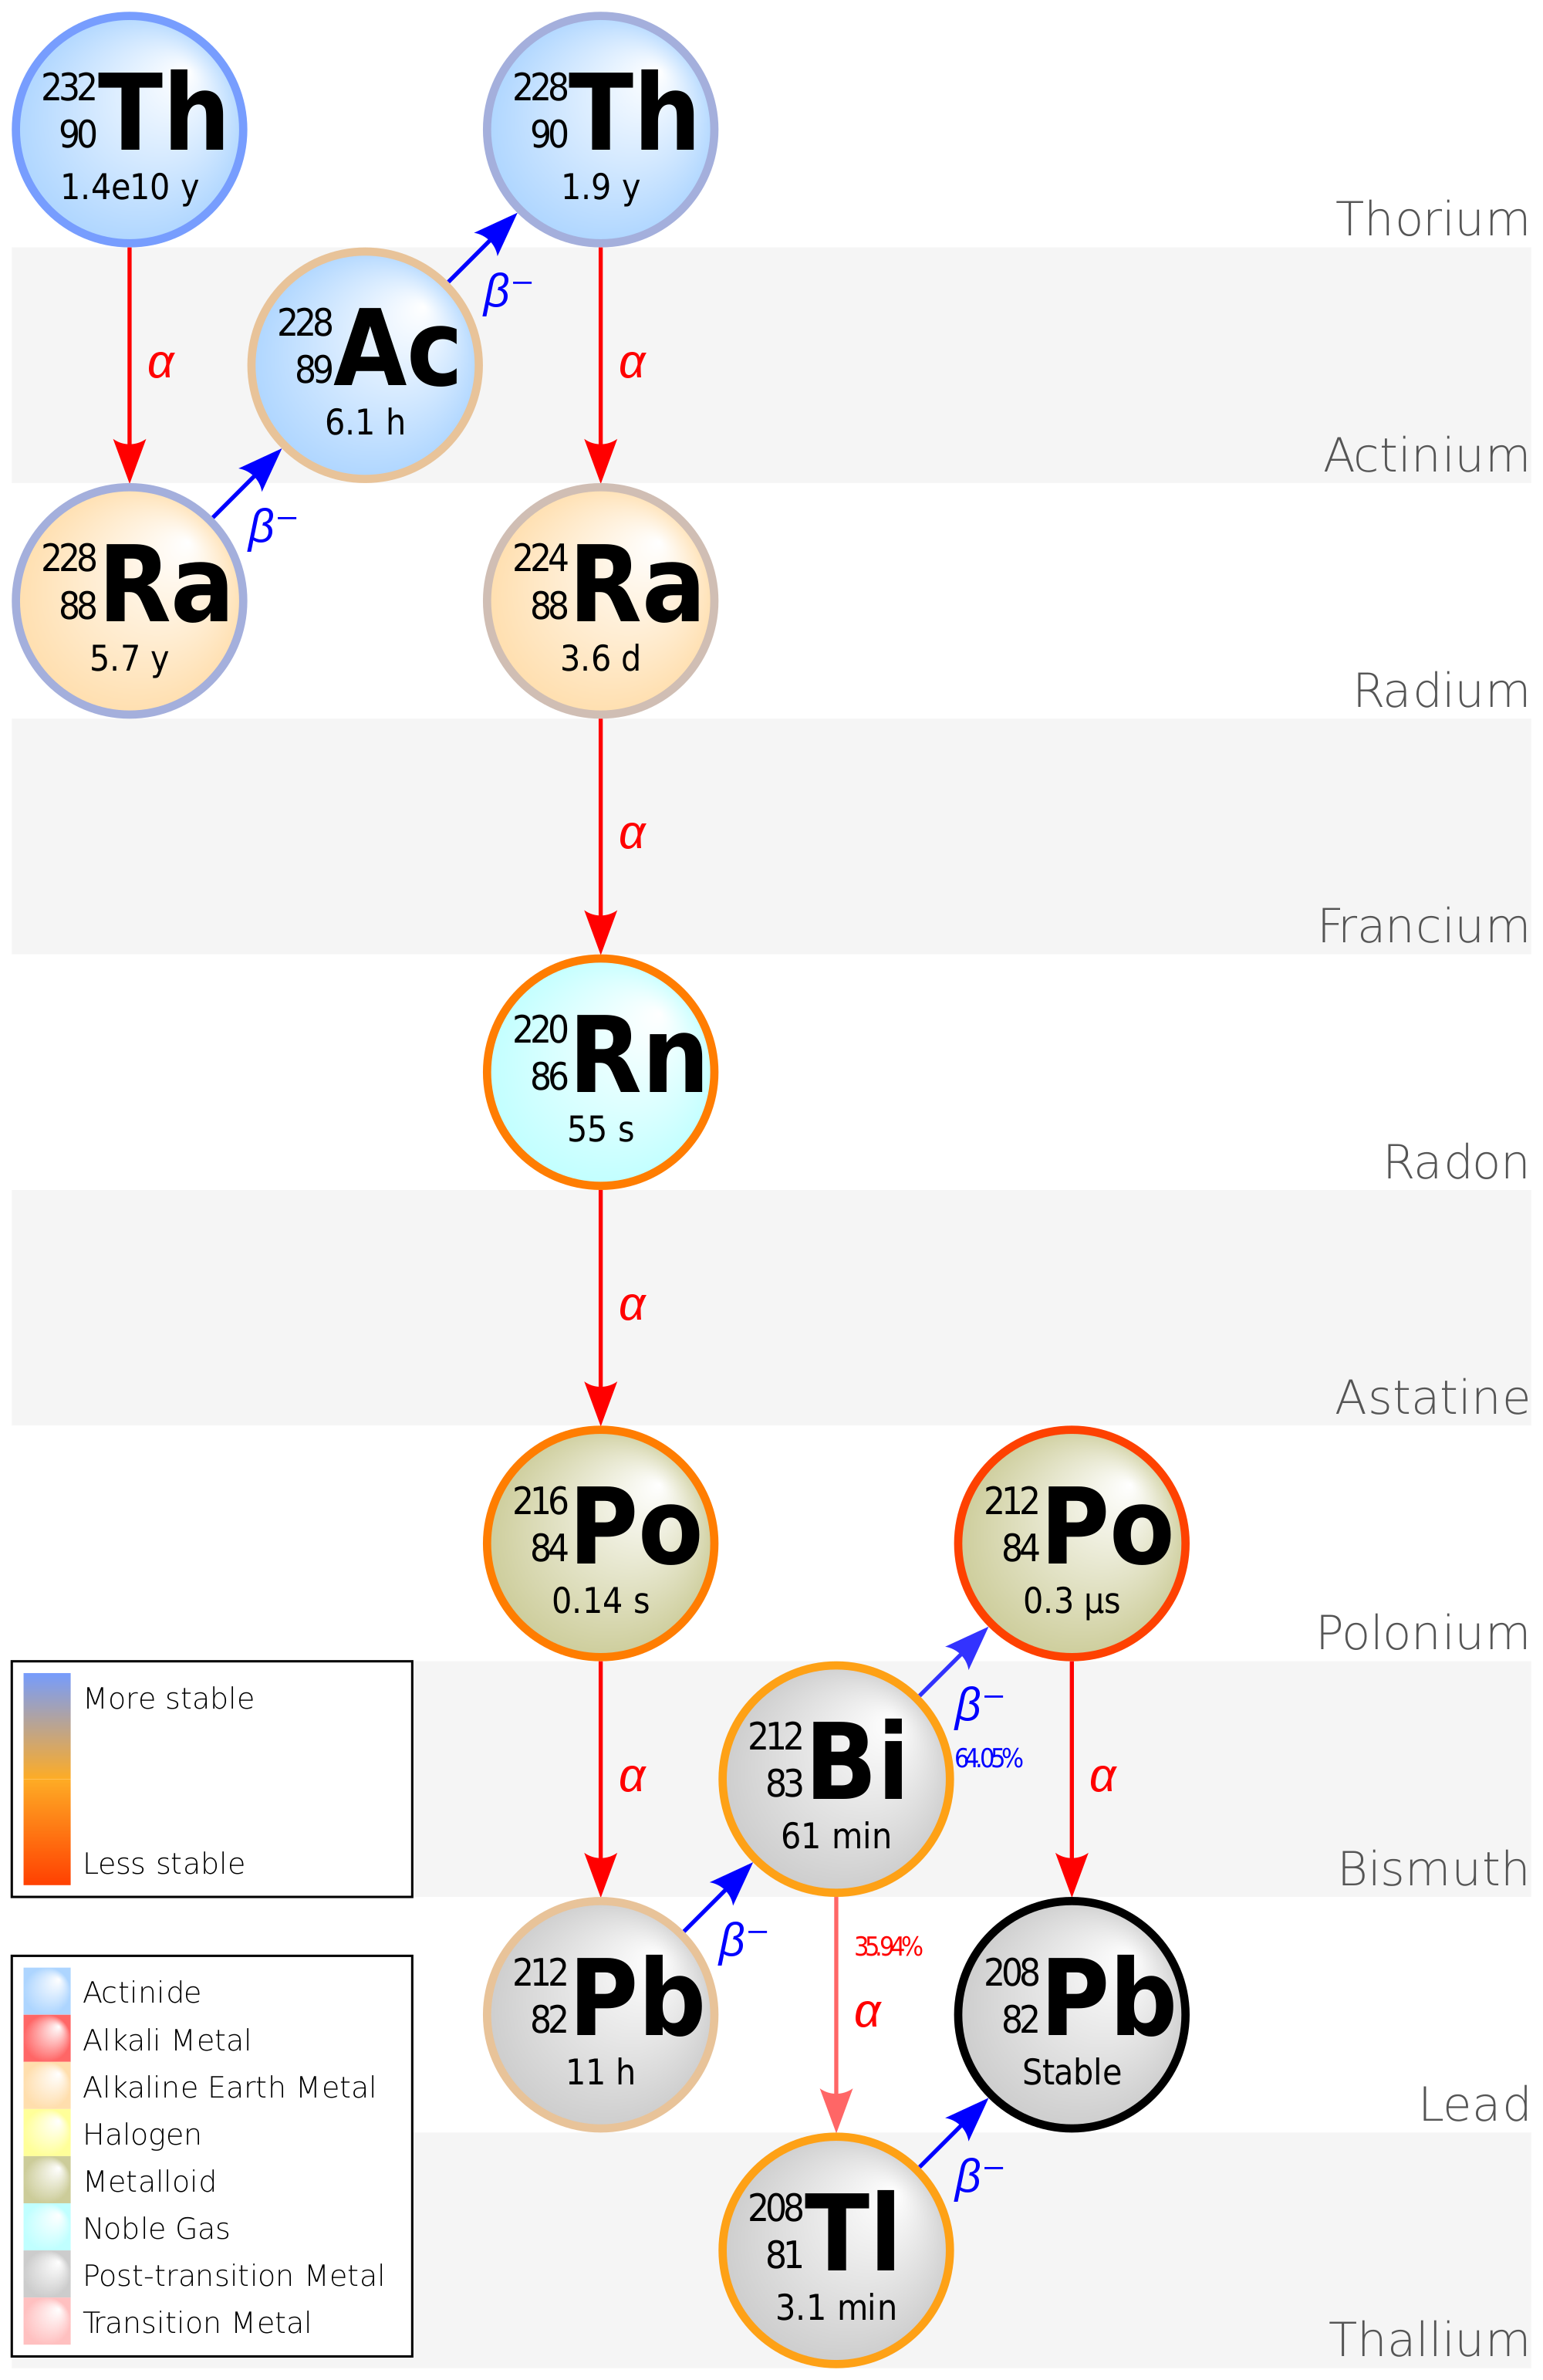
\includegraphics[width=\textwidth]{Decay_Chain_of_Thorium-232}
    \end{subfigure}%
    \begin{subfigure}[t]{0.5\textwidth}
        \centering
        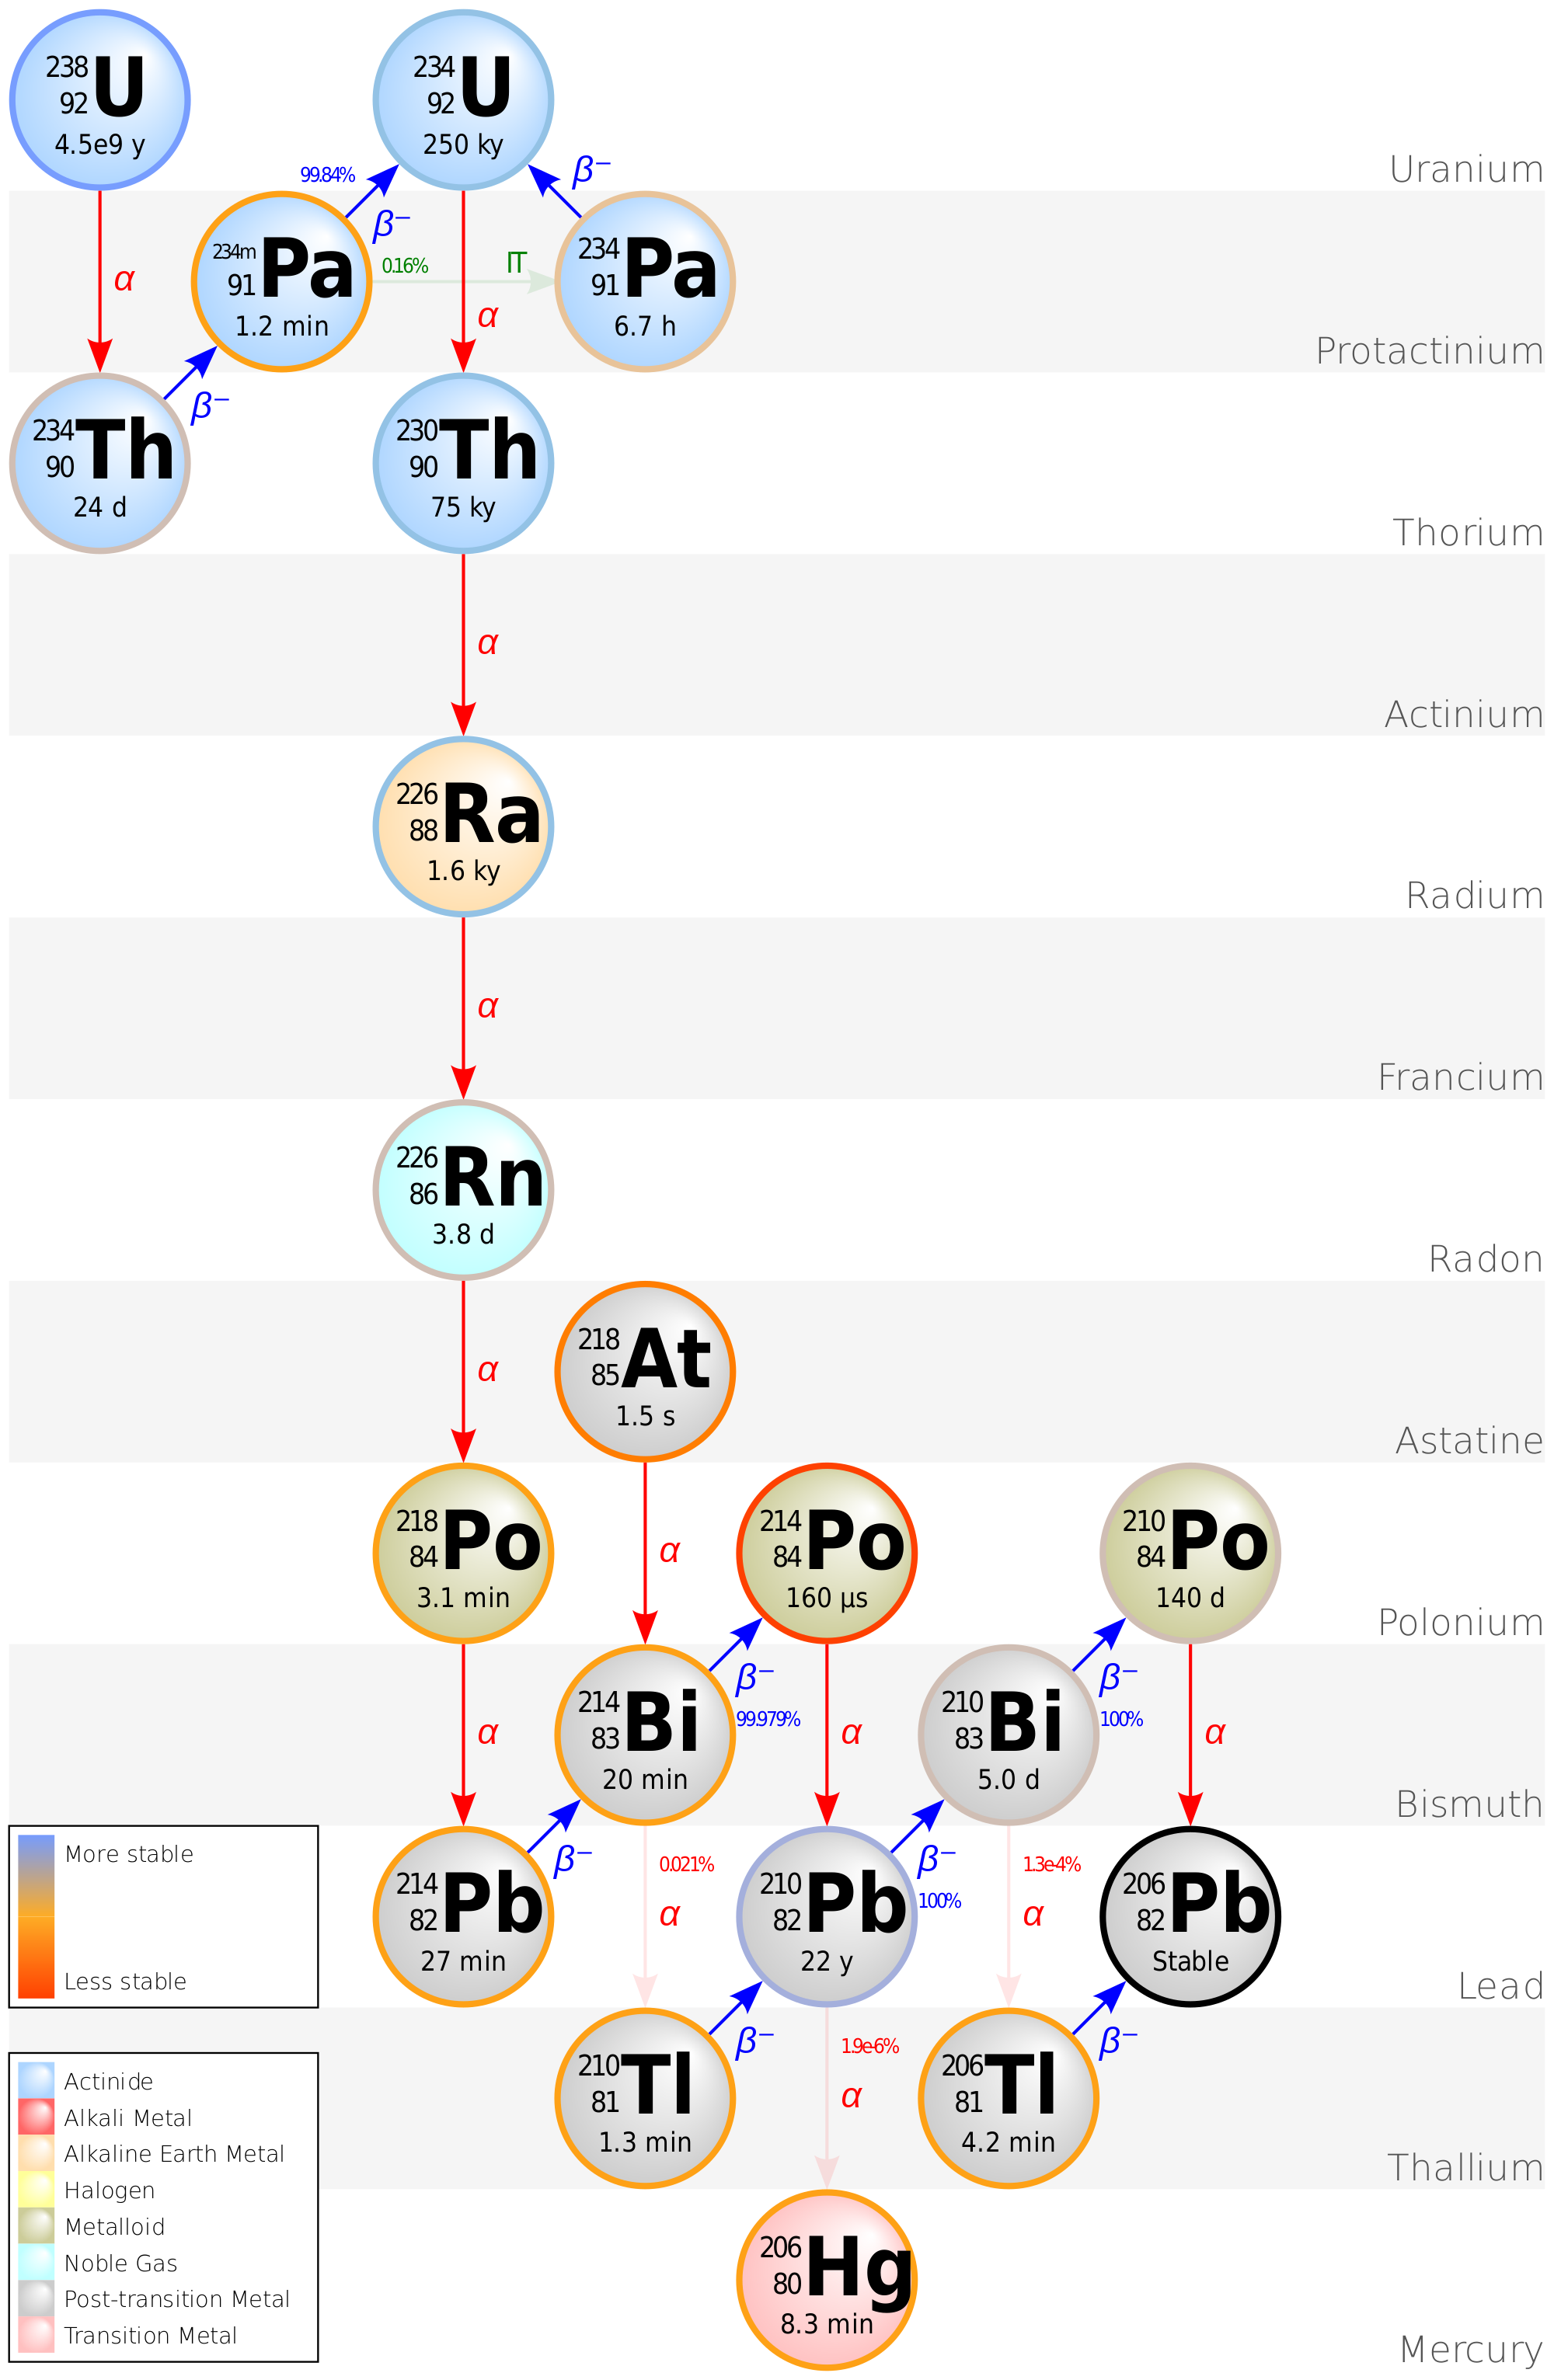
\includegraphics[width=\textwidth]{Decay_Chain_of_Uranium-238}
    \end{subfigure}
    \caption{Image credit: %https://commons.wikimedia.org/wiki/File:Decay_Chain_of_Uranium-238.svg
    .}
	\label{fig:backgrounds_decay_chains}
\end{figure}

\begin{figure}
\centering
\includegraphics[width=\textwidth]{WallChargingPlot}
\label{fig:backgrounds_wall_charge}
\end{figure}


\subsection{Electronic Recoils}
\label{subsec:backgrounds_electronic}
While the majority of total background events come from detector materials (\secref{backgrounds_detector_materials}) and are stopped
within the first few cm of LXe, there is a population distributed roughly uniformly throughout the LXe.  They are either noble gases (trace
amounts left from commercial distillation) - and therefore cannot be removed by the purification system - or neutrinos passing through the
Earth.  Because they exist everywhere in the LXe it is not possible to remove them with a FV cut.

\subsubsection{\ce{^{85}Kr}}
\label{subsubsec:backgrounds_electronic_krypton}
With a half-life of 10.76 y and $\beta^-$-decay end-point energy of 687 keV, \ce{^{85}Kr} is a concern for LXe dark matter
experiments.  It decays to \ce{^{85}Rb}, which itself is stable.  Mainly
produced by \ce{^{235}U} and \ce{^{239}Pu} in nuclear fission and then released by nucelar weapons tests and fuel reprocessing plants,
measurements show that $\mathrm{^{85}Kr / ^{nat}Kr} = 2 \times 10^{-11}$ (\citeref{Du2004}).  Its long half-life and low-energy
contamination threaten WIMP DM searches, especially if \ce{^{nat}Kr}/\ce{Xe} is left at the ppm to ppb level.  As discussed in
\secref{subsec:xenon1t_kr_dist} a krypton distillation column was installed in the service building and connected to the cryostat through
the purification system.  In the first science run a level of $0.36 \pm 0.06\ \mathrm{ppt}$ was reached, corresponding to a rate of
around 50 low-energy electronic recoils per year in a FV of 1 ton.

\subsubsection{\ce{^{222}Rn}}
\label{subsubsec:backgrounds_electronic_radon}
The largest intrinsic background comes from \ce{^{222}Rn}, which is part of the \ce{^{238}U} chain.  Although it has a half-life of only
3.8 days it can diffuse through the vacuum seals or emanate from the detector materials and gas system, keeping the fractional content in
equilibrium.  As mentioned in \secref{subsec:xenon1t_kr_dist} the Kr column was used to remove Rn during the first science run, though the
relative decrease was significantly smaller than with Kr.

\ce{^{222}Rn} undergoes $\alpha$-emission and therefore is not a danger to a WIMP search.  However, there are two daughters that undergo
$\beta^-$-decay: \ce{^{214}Pb} and \ce{^{214}Bi} (\ce{^{210}Tl} is also a $\beta^-$-emitter but has a branching ratio of just
0.021\%).  The most dangerous is the decay of \ce{^{214}Pb} to the ground state of \ce{^{214}Bi}, with an end-point energy of 1019 keV and
branching ratio of 10.9\%.  In the right panel of \figref{fig:backgrounds_er_spectrum} we can see that it is the leading contributor to
the ER
background rate.  The $\beta^-$-decay of \ce{^{214}Bi} is not concerning because its daughter, \ce{^{214}Po}, has a half-life of
$164.3\ \mathrm{\mu s}$ so a simple coincidence cut can remove the events.

\ce{^{220}Rn} has a half-life of just 55.6 s so it is much less likely to spread in the LXe active volume.  Its daughter, \ce{^{216}Po},
is more likely to bond to the detector wall.  However, \ce{^{220}Rn} is used in calibrations to study the electronic recoil band, which is
discussed in detail in \secref{subsec:er_nr_calibrations_rn220}.

Both Rn chains have a number of $\alpha$-decays - primarily from Rn and Po isotopes.  These can be useful in studying properties of the
detector (e.g. the wall charging mentioned in \secref{subsubsec:backgrounds_electronic_kr}) and also monitoring parameters such as
the electron lifetime.

\begin{figure}
    \centering
    \begin{subfigure}[t]{0.45\textwidth}
        \centering
        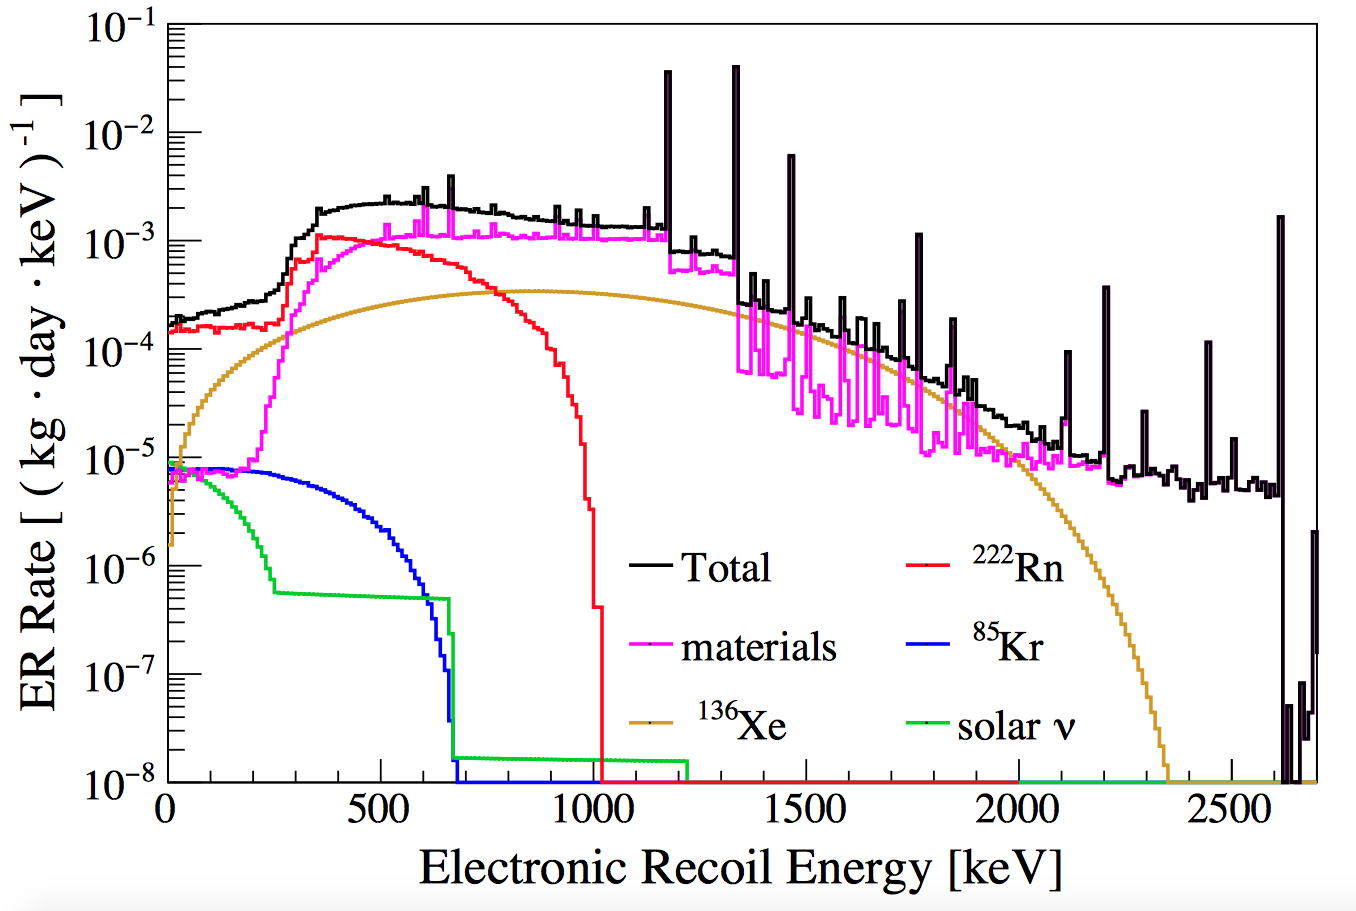
\includegraphics[height=4.5cm]{ERRateMCFull}
    \end{subfigure}%
    \begin{subfigure}[t]{0.45\textwidth}
        \centering
        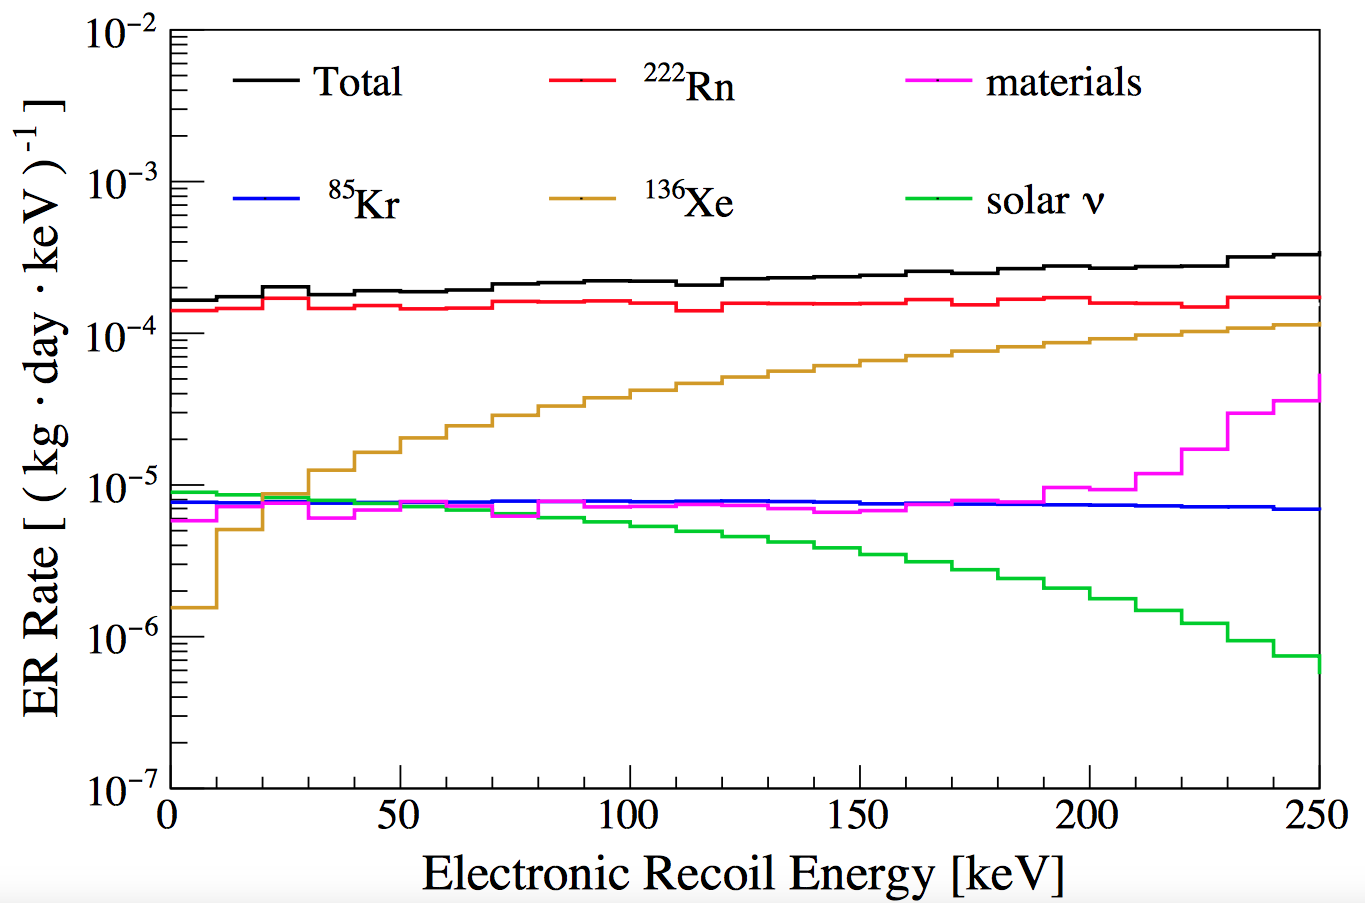
\includegraphics[height=4.5cm]{ERRateMCZoomed}
    \end{subfigure}
    \caption{Image credit: %https://commons.wikimedia.org/wiki/File:Decay_Chain_of_Uranium-238.svg
    .}
	\label{fig:backgrounds_er_spectrum}
\end{figure}



\subsubsection{\ce{^{136}Xe}}
\label{subsubsec:backgrounds_electronic_xe}
\ce{^{136}Xe} is the only unstable isotope of natural xenon.  It undergoes $2 \nu \beta^- \beta^-$ decay with
$t_{1/2} = 2.17 \times 10^{21}\ \mathrm{years}$ (\citeref{Albert2014}) and a Q-value of 2458 keV.  Because of its abundance in natural
xenon (\ce{^{136}Xe}/\ce{Xe} = 8.9\%) its presence is unavoidable.  At the scale of XENON1T it is subdominant - only responsible for
${\sim}2 \%$ of the total ER background, as seen in \figref{fig:backgrounds_er_spectrum} (right).  However, as detectors continue to grow
it will become much more consequential.



\subsubsection{Solar Neutrinos}
\label{subsubsec:backgrounds_electronic_solar_neutrinos}
Solar neutrinos can elastically scatter off electrons, causing low-energy electronic recoils.  The recoil spectrum is the green line in
\figref{fig:backgrounds_er_spectrum}.  As with the \ce{^{136}Xe} $2 \nu \beta^- \beta^-$
decay its contribution is small, but as an irreducible background it will become more problematic as detectors grow.



\subsection{Nuclear Recoils}
\label{subsec:backgrounds_nuclear}
Our nuclear recoil background comes from neutrons and neutrinos.  Whereas \gammarays are stopped within several cm, high-energy neutrons
have mean free paths of $\mathcal{O}(10)$ cm, allowing them to move through the LXe volume more easily and giving a higher probability
that it scatters once inside the FV.  Neutrinos move freely and cannot be shielded.  The nuclear recoil background is composed of
radiogenic and muon-induced neutrons as well as from astrophysical neutrinos.



\subsubsection{Radiogenic Neutrons}
\label{subsubsec:backgrounds_nuclear_radiogenic}
Radiogenic neutrons are produced by primordial decay chains \ce{^{238}U}, \ce{^{235}U} and \ce{^{232}Th} in detector materials
(see \secref{subsec:backgrounds_detector_materials} for discussion on electronic and $\alpha$ recoils).  They are released in
$(\alpha, \mathrm{n})$ reactions that result from the $\alpha$-emissions along the decay chains, as well as spontaneous fission (SF).  For
heavier nuclei radiogenic neutrons are generated almost exclusively by SF as the $(\alpha, \mathrm{n})$ reaction is suppressed by the
large Coulomb barrier (\citeref{Aprile2016a}).

\figref{fig:backgrounds_nuclear_radiogenic_rates} shows the neutron yield as a function of energy for PTFE and copper from Monte Carlo
predictions.  The chains are
separated to $\mathrm{^{238}U} \rightarrow \mathrm{^{230}Th}$ and $\mathrm{^{226}Ra} \rightarrow \mathrm{^{206}Pb}$, and
$\mathrm{^{232}Th} \rightarrow \mathrm{^{228}Ac}$ and $\mathrm{^{228}Th} \rightarrow \mathrm{^{208}Pb}$ to account for the disequilibrium
that was observed.  The PTFE has on average a lighter $Z$ than the copper, giving it a larger $(\alpha, \mathrm{n})$ contribution (dashed
lines represent SF-only).  We can see in \figref{fig:backgrounds_nuclear_muon_induced_nr_rate} that for $E \gtrsim 3\ \mathrm{keV}$
radiogenic neutrons are the dominating factor for the NR backgrounds.  The expected rate for 1 ton is
$0.6 \pm 0.1\ \mathrm{y^{-1}}$.

\begin{figure}
\centering
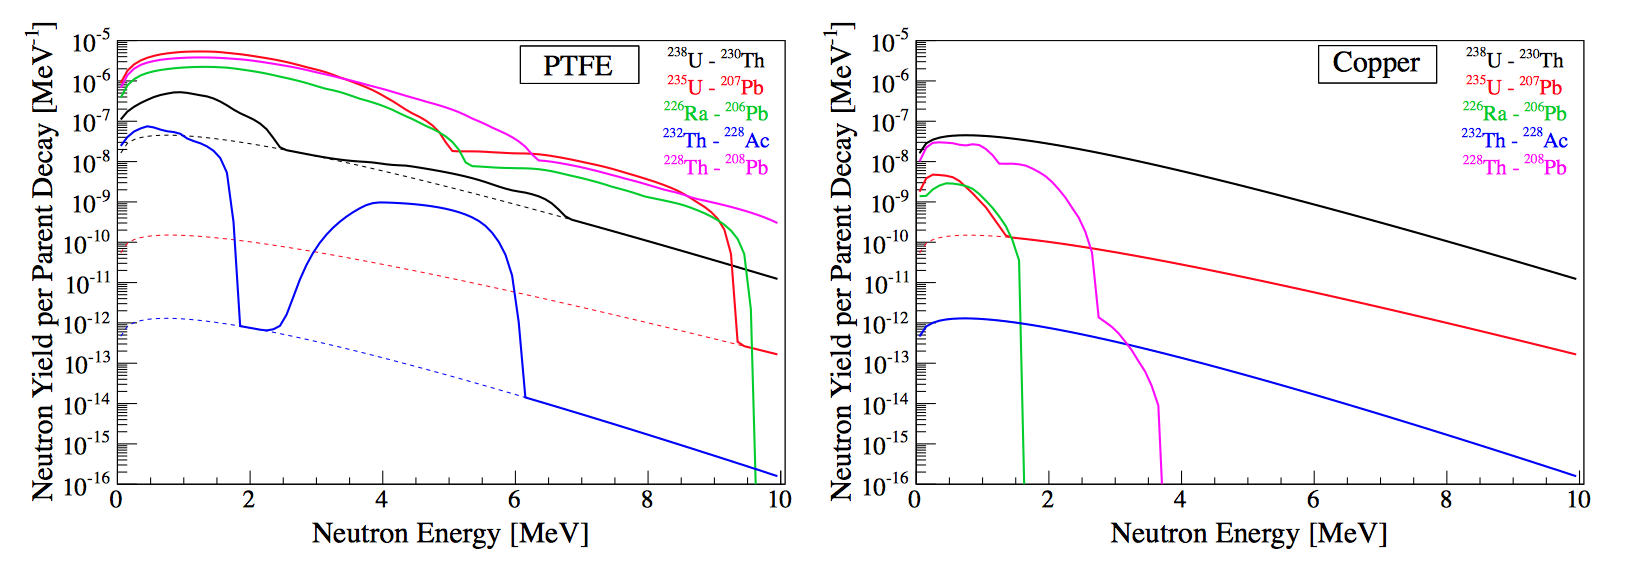
\includegraphics[width=\textwidth]{NeutronYields}
\caption{Image credit: \citeref{Aprile2016a}.}
\label{fig:backgrounds_nuclear_radiogenic_rates}
\end{figure}



\subsubsection{Muon Induced Neutrons}
\label{subsubsec:backgrounds_nuclear_muon_induced}
Cosmic muons interacting with the rock above the detector can produce up to GeV neutrons.  The large mean free path from such high energy
makes it not unlikely that they pass through the water shield (\secref{subsec:xenon1t_water_shield}).  However, simulations show that if
the associated showers from the muon interaction also enter the tank the tagging efficiency is $> 70\%$.  Still the predicted rate is just
$< 0.01\ \mathrm{y^{-1}}$ for 1 t and is represented by the blue line in \figref{fig:backgrounds_nuclear_muon_induced_nr_rate}.

\begin{figure}
\centering
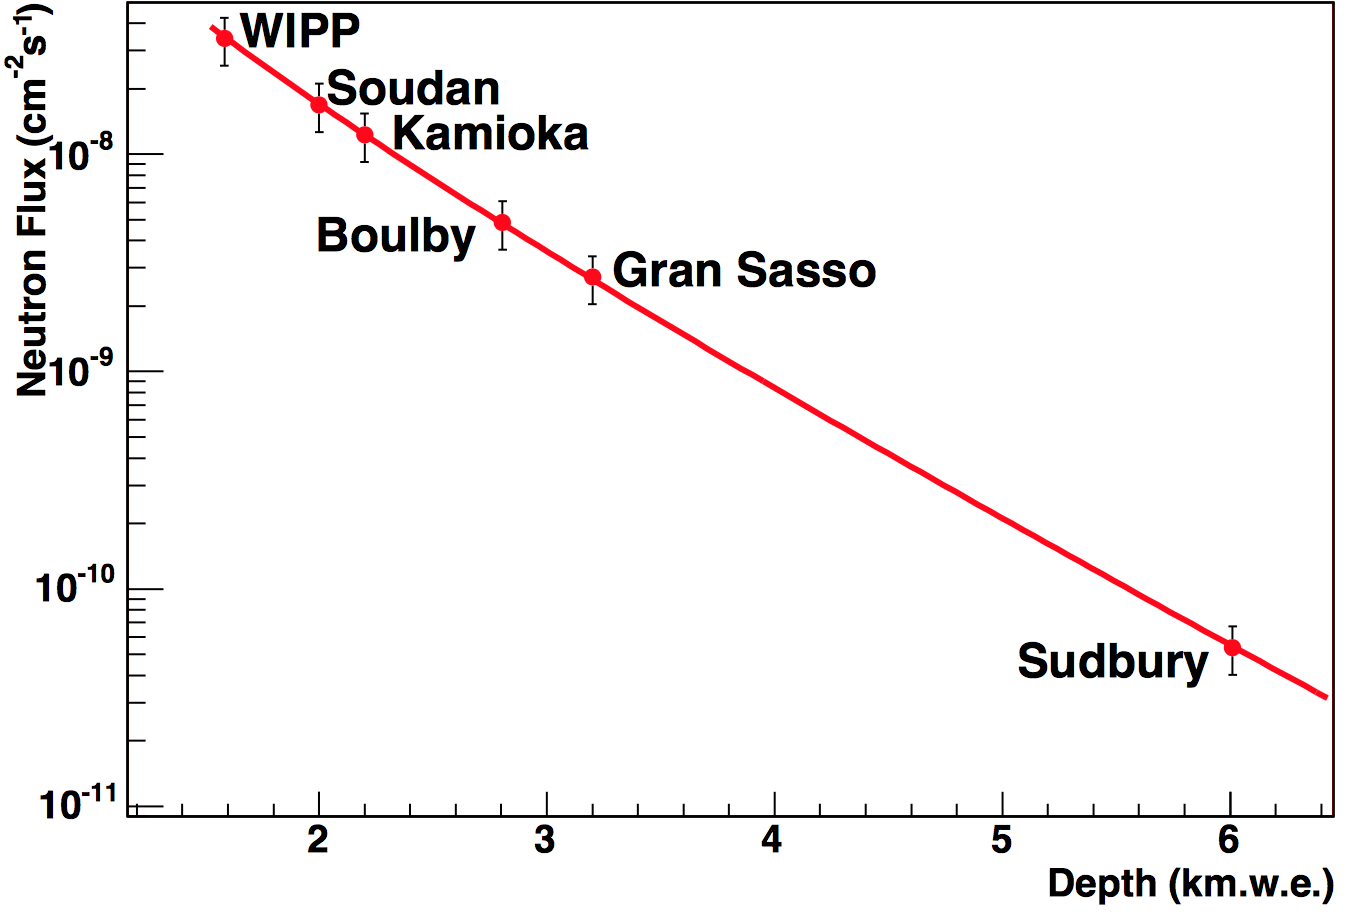
\includegraphics[width=0.8\textwidth]{MuonFluxOverDepth}
\label{fig:backgrounds_nuclear_muon_induced_flux}
\end{figure}

\begin{figure}
\centering
\includegraphics[width=\textwidth]{Fig7Aprile2016a}
\caption{Image credit: \citeref{Fig7Aprile2016a}.}
\label{fig:backgrounds_nuclear_muon_induced_nr_rate}
\end{figure}



\subsubsection{Neutrinos}
\label{subsubsec:backgrounds_nuclear_neutrinos}
The final contribution to the NR background comes from neutrinos that participate in coherent neutrino-nucleus scattering.  The primary
contributor to the integrated NR rate is solar \ce{^{8}B}, which is orders of magnitude larger than other sources and dominant at
recoil energies $< 3\ \mathrm{keV}$.  Solar $hep$, atmosphere, and diffuse supernova neutrinos also contribute.  We can see in
\figref{fig:backgrounds_nuclear_muon_induced_nr_fate} that neutrinos are the principal source for recoils at $< 3\ \mathrm{keV}$.  The
number of detected events at $> 1\ \mathrm{keV}$ was predicted to be ${\sim} 90\ \mathrm{t^{-1}\ y^{-1}}$.  While this is below our
threshold, Poissonian variations may put a small fraction into our detection region.  By looking at the expected number of events closer
to our threshold (${sim} 4\ \mathrm{keV}$) this drops to $1.8 \times 10^{-2}\ \mathrm{t^{-1}\ y^{-1}}$.  As mentioned in
\secref{subsubsec:backgrounds_electronic_solar_neutrinos} neutrinos will compose a greater fraction of our background due to the inability
to shield them.



\section{Detector Characterization}
\label{sec:det_char}
Calibrations allow detector characterization and monitoring as well as measurement of fundamental physics.  In XENON1T calibrations have
been done with $\mathrm{^{83m}Kr}$, \ce{^{222}Rn}, \ce{^{137}Cs}, \ce{^{228}Th}, Americium beryllium, a neutron generator, and LEDs.
% look at http://www.uni-muenster.de/Physik.KP/AGWeinheimer/Files/theses/Bachelor_Sergej_Schneider.pdf sections 2.2 and 2.3


\subsection{PMT Gain}
\label{subsec:det_char_pmt_gain}
The charge that reaches the anode can change for a single phototube and varies between different.  Increasing the bias voltage amplifies
the gain, heightening sensitivity or conversely lowering can help prevent saturation.  Gains may also deviate from variations in
temperature (\textbf{check this}), overexposure to light, count rate, wear, and more.  Phototubes may differ from one another
for all the reasons just mentioned, as well as inevitable - however tiny - differences in parts.  Monitoring the single photoelectron (SPE)
response for each PMT then is essential for accurately reconstructing the number of photoelectrons and by extension the energy of the
event.  This is typically done with an LED inside the TPC.  Typically blue light is used since ultraviolet is unavailable, which despite
being far outside of the 178 nm range ejects a photoelectron some small fraction of the time.  Each time the LED flashes we can record the
PMTs (during normal data taking this requires a pulse larger than some threshold, \secref{}).  After a large ($\mathcal{O}(10^{5})$)
number of trials a histogram can be fit to find the SPE gain as shown in \figref{fig:xenon1t_pmt_spe}.  Note that technically the charge
is plotted but the gain is easily found as $g = \mu_{e} / e$ where $\mu_{e}$ is the mean number of \electron and $e$ is the electron charge.  We
see a large peak centered at 0 that corresponds to the baseline noise when a photoelectron is not released.  At larger gain a series of
smaller wider peaks are visible that represent integer numbers of photoelectrons, starting with 1 at the leftmost.  There is a ``shoulder"
between the baseline and first peak that cannot be explained by only considering signal from integer PEs.  As briefly mentioned in
\secref{subsec:tpcs_pmts} this comes from photons that pass through the photocathode and free an electron on the first dynode, causing an
under-amplified charge.  This is generally the most challenging aspect to model.

\begin{figure}
\centering
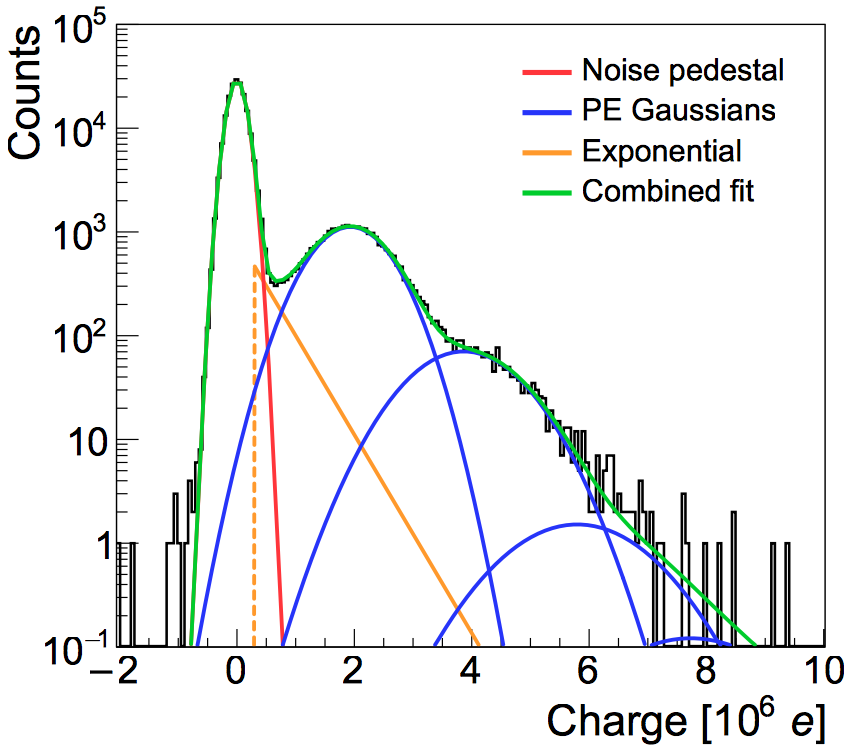
\includegraphics[width=0.6\textwidth]{SPESpectrum}
\caption{(Left) Single photoelectron spectrum.}
\label{fig:xenon1t_pmt_spe}
\end{figure}

In \figref{fig:xenon1t_pmt_spe} the spectrum is fit assuming the noise baseline and PE peaks are gaussian and the under-amplification is
an exponential.  The PE gaussians are constrained by $\mu_{N} = N \mu_{e}$ and $\sigma_{N} = \sqrt{N} \sigma_{e}$ where $\sigma_{e}$ is the
standard deviation of the single photoelectron peak and $\mu_{N}$ and $\sigma_{N}$ are the mean and standard deviation for the peak with
$N$ photoelectrons.  As this model is simplistic and can add bias recent efforts have gone in to alternative methods
of characterization (\secref{Saldanha2017, 2017Anthony}).  Nonetheless, the combined fit (green) appears to agree will with the data.

We can use the SPE spectrum to calculate the resolution $R = \sigma_{e} / \mu_{e}$.  As the gain grows the resolution should sharpen
initially until it eventually levels off.  For the R11410-21 models the plateau began around $2 \mdash 3 \times 10^{6}$ at a resolution of
27\%.  Because the stress on the PMT raises with bias voltage and larger gains lead to greater saturation we decided there was no benefit
to exceeding this gain.

\begin{figure}
\centering
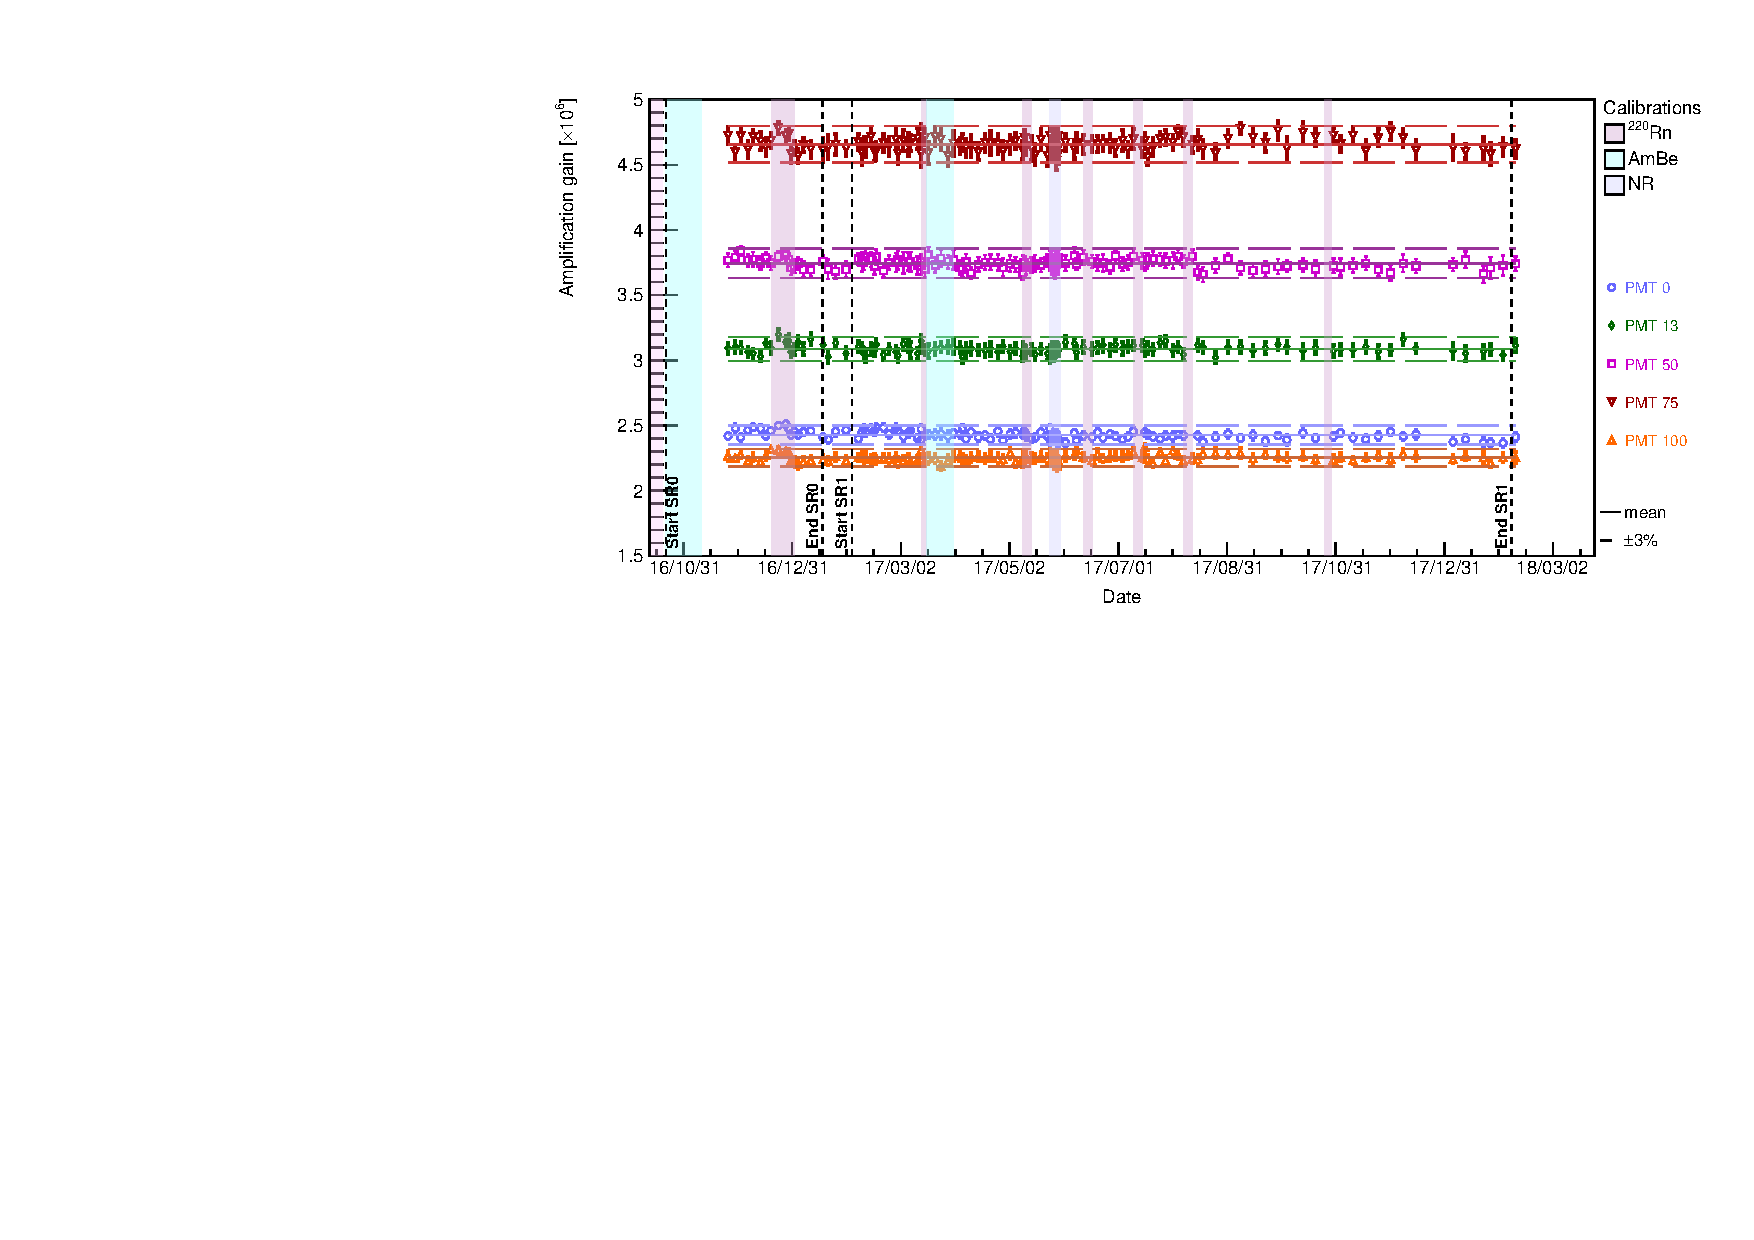
\includegraphics[width=\textwidth]{PMTGainStability}
\caption{Gains for five PMTs monitored from SR0 until the end of SR1.  Means and $\pm 3\%$ are shown.  All appear to be stable.}
\label{fig:xenon1t_pmt_time}
\end{figure}

The relatively poor resolution is apparent in \figref{fig:xenon1t_pmt_spe} as the photoelectron peaks are hard to distinguish.  An
important metric of the SPE spectrum is the peak-to-valley ratio, which divides the first PE peak by the valley that sits between it and
the baseline noise.  As with $R$ it increases for low gains and eventually levels.  For gains of $2 \mdash 3 \times 10^{6}$ the mean
peak-to-valley ratio is ${\sim} 3$.  The PMT gains are regularly measured to identify any changes in gain.  This is shown for five
PMTs - all of which are stable - in



\subsection{$\mathrm{^{83m}Kr}$}
\label{subsec:det_char_kr}
The most common calibration source is $\mathrm{^{83m}Kr}$.  Being a noble gas it can be injected directly into the xenon so to be used as an
internal calibration.  \ce{^{83}Rb} is installed in a source box connecting to the purification system
(\secref{subsec:xenon1t_calibrations_internal}) and decays through electron capture

\begin{equation}
\mathrm{^{83}Rb} + e^- \rightarrow \mathrm{^{83}Kr} + \nu_e
\end{equation}

with a 74.8\% branching ratio to the metastable state $\mathrm{^{83m}Kr}$.  $\mathrm{^{83m}Kr}$ then de-excites in two steps: emission of a 32.1 keV
conversion electron with half-life $t_{1/2} = 1.83\ \mathrm{h}$ followed by a second conversion electron at 9.4 keV with
$t_{1/2} = 154\ \mathrm{ns}$.  The short
interval between the two decays makes tagging events easy.  Furthermore the mono-energetic $\gamma$ lines can be used for a number of
detector characterizations including light collection efficiency (LCE), S2 position correction maps, position reconstruction, and electron
lifetime.

\subsection{Light Collection Efficiency}
\label{subsec:det_char_lce}
The light observed by a PMT depends on - among other things - the position of the event.  The light collection efficiency (LCE) - seen
in \figref{calibrations_lce_lce} - quantifies these differences.  Such position-dependent variations exist simply because the location of
the interaction dictates subsequent effects due to detector features and physics.  First, the the solid angle of an event is not uniform
throughout the detector.  It is greatest near the bottom or top of the TPC at small radii.  The measured strength of the scintillation
from the S1 depends then on the number of PMTs the light can reach and how far the light must travel to each.  Interactions near the
wall have a lower observed intensity because of this.  The quantum efficiency (QE) of the PMTs (\figref{fig:xenon1t_pmt_array}) is also a
factor, with those at larger values more likely to produce a photoelectron.  Because the PMTs with the highest QE were placed in the
center of the bottom array (\secref{subsec:xenon1t_pmts}) events that happen near there should have a higher likelihood of detection,
while those in in near the top corners should have the lowest.

Because PTFE has some small but $> 0$ absorption the intensity of the scintillation decreases with each reflection.  Therefore light
that is emitted perpendicular to the PMT arrays can be severely dampened.  This is amplified by the absorption of light by
impurities in the LXe, meaning that longer traversed distances imply decreased scintillation.

The index of refraction of LXe ${\sim} 1.7$
gives a critical angle $\theta_c = 36^{\circ}$.  The light then that reaches the top PMTs for an event at
$z = -10\ \mathrm{cm}$ is restricted to a radius of just 13.6 cm at the liquid surface, with the total solid angle from
$r = 0\ \mathrm{cm}$ of $83.9^{\circ}$.  While the light will be internally reflected and progress towards the bottom array, it is likely
to be lessened from reflections with the PTFE and extended travel distances as discussed in the previous paragraph. In comparison light
directed towards the surface from an event 10 cm above the cathode ($r = 0$)
has $< \theta_c$ everywhere.  Some scintillation that reflects off the PTFE on the way up will rebound off the surface, but its
contribution is relatively small.

\begin{figure}
    \centering
    \begin{subfigure}[t]{0.45\textwidth}
        \centering
        \includegraphics[height=4.5cm]{Fig20Aprile2017b}
        \label{fig:calibrations_lce_lce_hist}
    \end{subfigure}%
    \begin{subfigure}[t]{0.45\textwidth}
        \centering
        \includegraphics[height=4.5cm]{Fig21Aprile2017b} \\
        \label{fig:calibrations_lce_cle_map}
    \end{subfigure}
    \begin{subfigure}[b]{\textwidth}
        \centering
        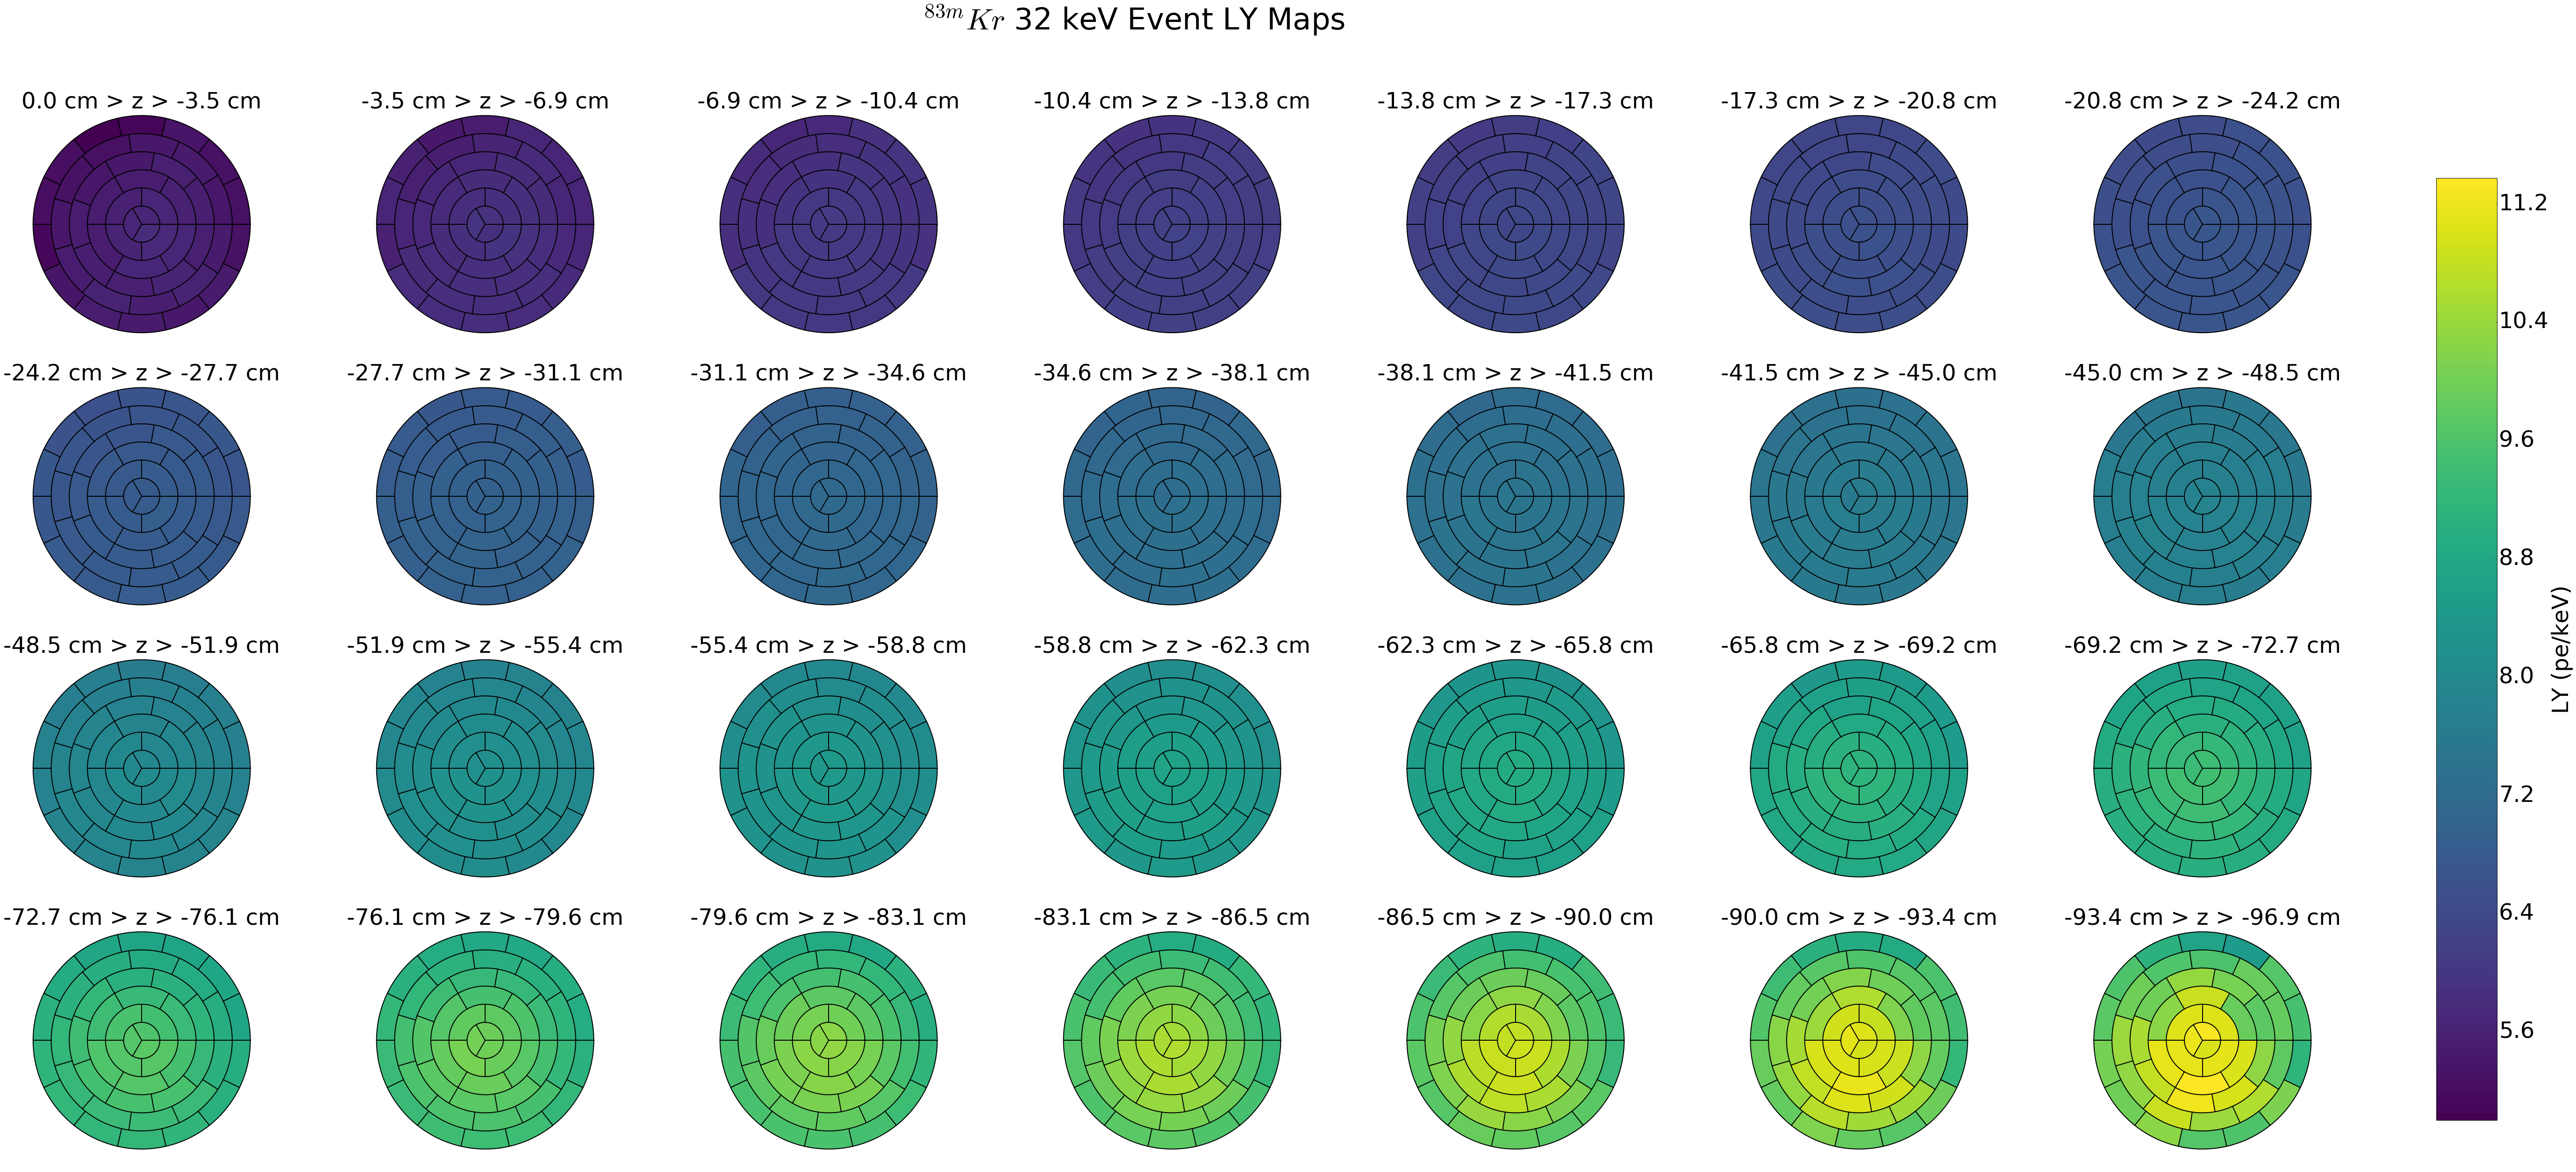
\includegraphics[height=4.5cm]{LCEMapPolar}
        \label{fig:calibrations_lce_cle_map}
    \end{subfigure}
    \caption{Image credit: \citeref{Aprile2017b}.}
	\label{fig:calibrations_lce_lce}
\end{figure}

\begin{figure}
\centering
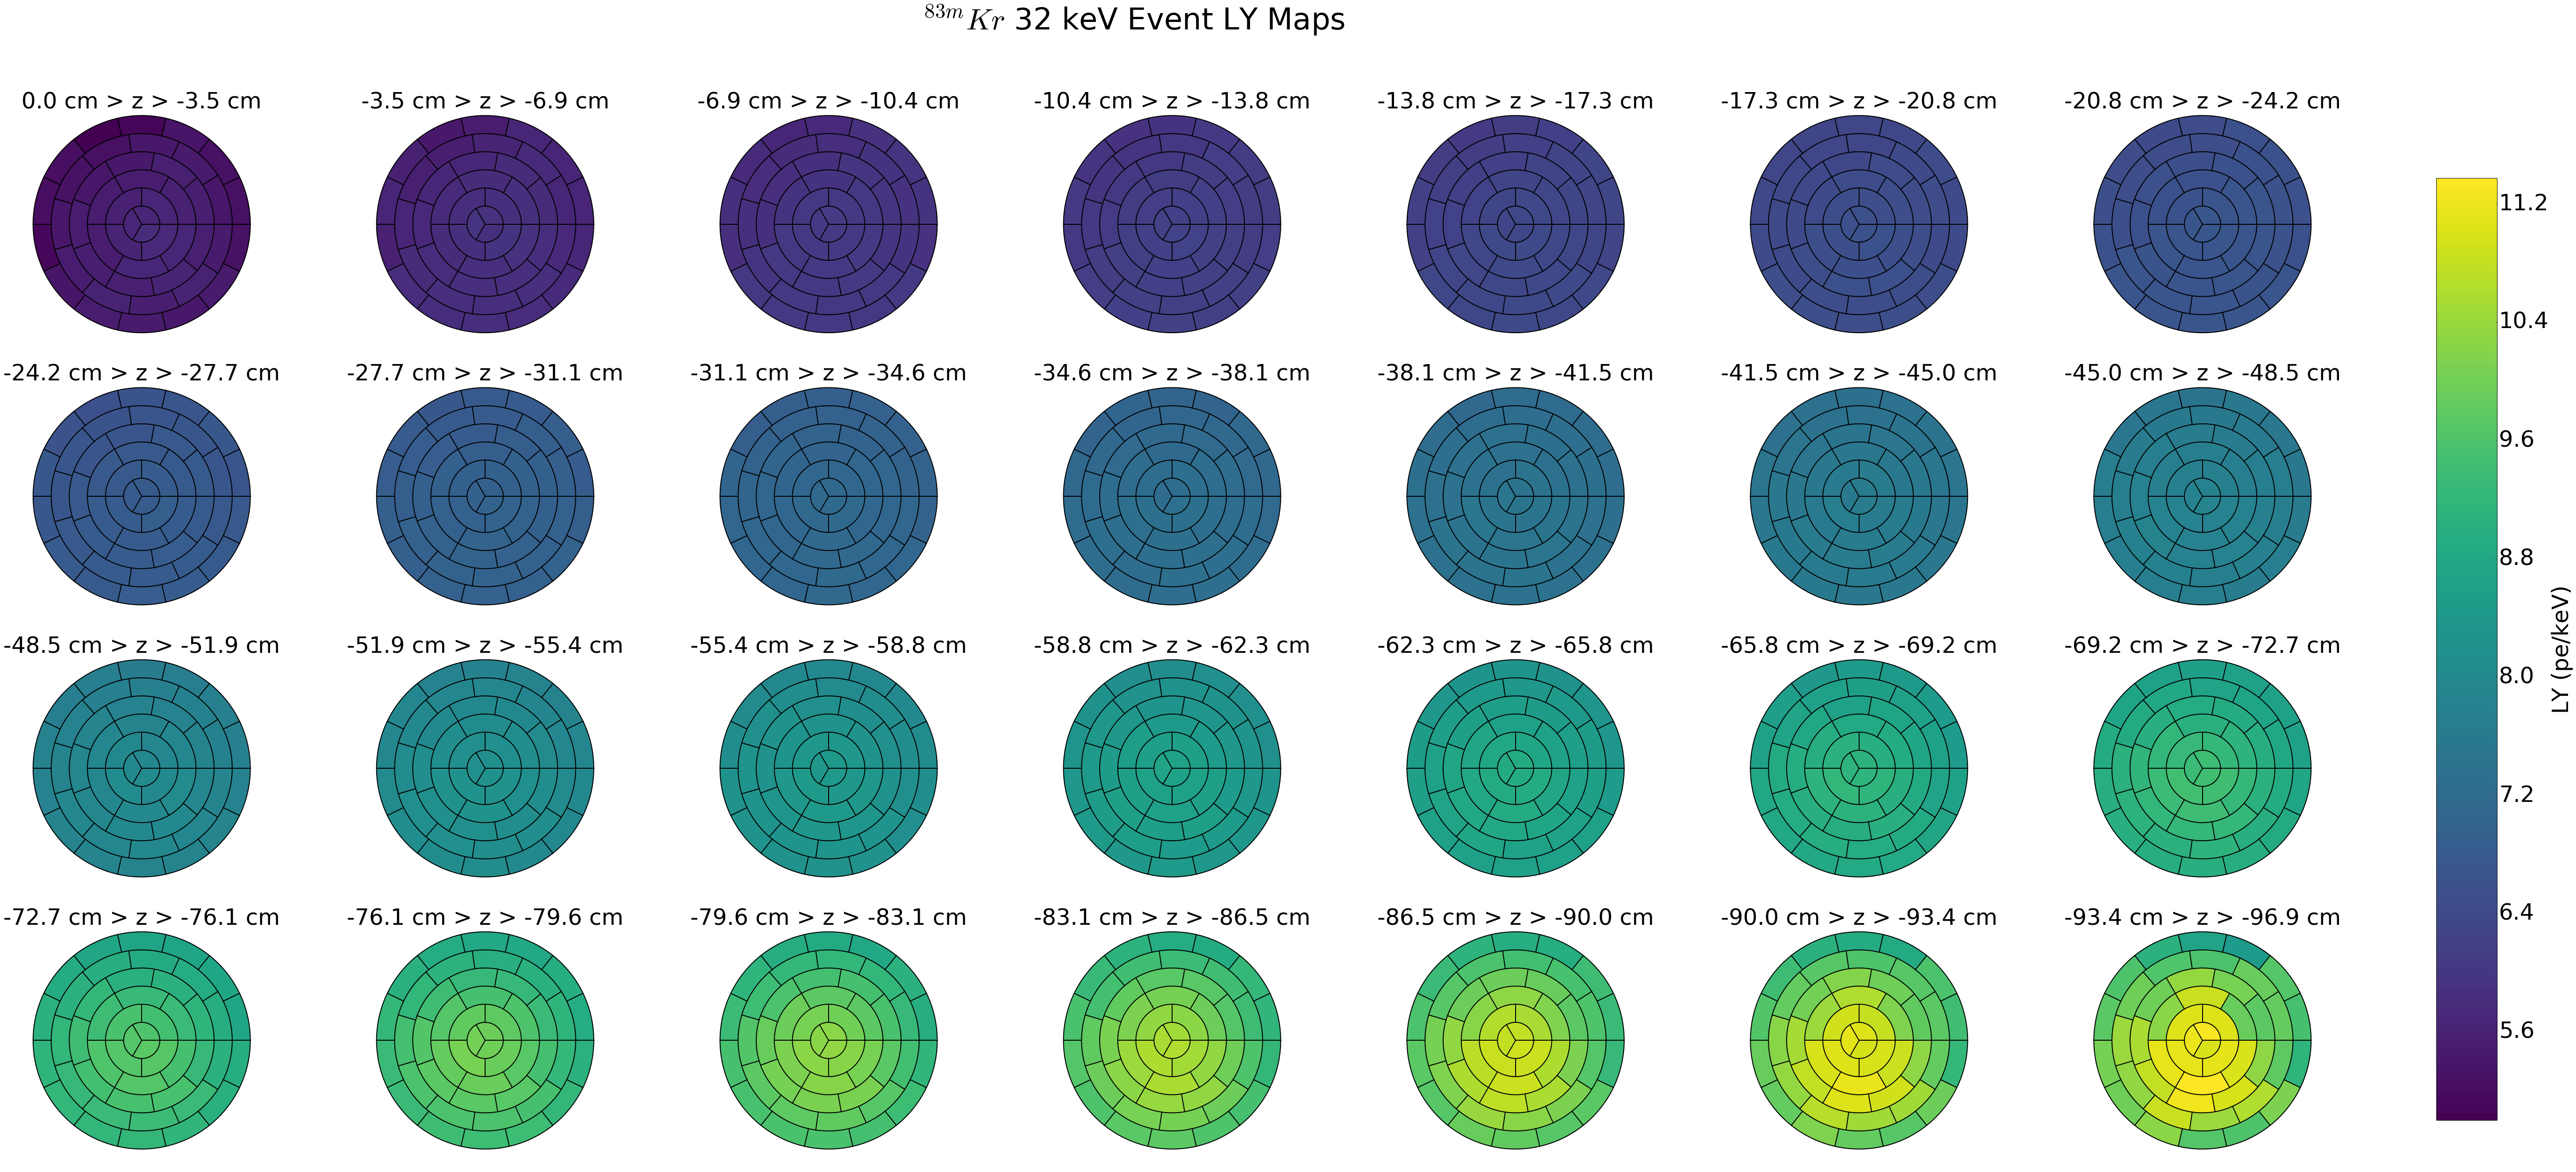
\includegraphics[width=\textwidth]{LCEMapPolar}
\caption{Light yield in slices of $z$ and $\phi$.}
\label{fig:calibrations_lce_polar}
\end{figure}

Calibrating the LCE requires a mono-energetic peak - preferably one near our DM energy range.  For this we use the light from the
$\mathrm{^{83m}Kr}$ 32.1 keV conversion electron.  The left panel in \figref{fig:calibrations_lce_lce} shows fits to S1s measured below the gate
(red), in the TPC center (blue), and above the cathode (green).  The mean from these fits correspond to the values shown in the right
panel.

It is important to point out that because recombination depends on recoil energy and electric field the derived LCE map is not
technically correct for other energies.  However, field non-uniformities are small, especially after more than a few cm inside of the
wall, so applying it universally is acceptable.

In the case of high-energy events PMT saturation can
affect the measured signal so the latter becomes important.



\subsection{S2 Position Correction}
\label{subsec:det_char_s2_position_correction}
We must also account for positional variations in S2.  However, because all S2s happen in the GXe an $x-y$ correction is sufficient.  For
this we use the 41.5 keV peak of $\mathrm{^{83m}Kr}$ (the 154 ns half-life of the 9.4 keV decay makes it difficult to separate the two
S2s).  Most of the light seen by the top array is focused on a small group of PMTs directly over the extraction site, while the light on
the bottom array is more uniformly spread due to a larger solid angle.

The top and bottom correction maps are shown in \figref{fig:calibrations_s2_maps}.  The local variations are primarily
caused by nonfunctional PMTs.  The observed signal in the top array being more densely concentrated causes steeper local variations.  The
slightly higher S2s at low radii result from a small sagging of the anode.  The increase in the bottom array as $r \rightarrow 0$ is 
mainly due to the higher QE.  The large solid angle creates a roughly homogeneous azimuthal distribution.

\begin{figure}
    \centering
    \begin{subfigure}[t]{0.45\textwidth}
        \centering
        \includegraphics[height=4.5cm]{S2MapTopUseDataFromBlessedPlots}
    \end{subfigure}%
    \begin{subfigure}[t]{0.45\textwidth}
        \centering
        \includegraphics[height=4.5cm]{S2MapBottom}
    \end{subfigure}
    \caption{}
	\label{fig:calibrations_s2_maps}
\end{figure}



\subsection{Position Reconstruction}
\label{subsec:det_char_position_reconstruction}
As mentioned in \secref{subsubsec:tpcs_signals_posrec} TPCs allow 3-dimensional position reconstruction.  Since the drift velocity $v_d$
is constant in LXe the depth is easily found as $z = -v_d t_d$ where $t_d$ is the drift time ($z$ is defined to be negative with
$z = 0$ at gate).  For Science Run 1 (SR1) the drift field $E_d = 81.3\ \mathrm{kV\ cm^{-1}}$ giving
$v_d = 1.332\ \mathrm{mm\ \mu s^{-1}}$ and maximum drift time of $727.3\ \mathrm{\mu s}$ (TPC drift length is 96.9 cm at
$-100^{\circ}\ \mathrm{C}$).

The $x-y$ coordinates are found by applying an algorithm to the intensity each PMT in the top array observed from the S2 (also known as
PMT hit pattern).  For XENON1T two reconstruction algorithms were mainly used.  The first was a neural net using the Fast Artificial
Neural Network (FANN) library with 24 and 29 nodes in the two hidden layers (sequentially).  The second matches the real hit pattern with
an expected after weighting four other algorithms for its seed, and is known as top pattern fit (TPF).  Both algorithms were trained on MC
and optimized with $\mathrm{^{83m}Kr}$ data, and achieved a position resolution of $\lesssim 2\ \mathrm{cm}$.  For SR1 the NN was ultimately
chosen, as the TPF algorithm was more sensitive to dead PMTs and showed some artificial discontinuity in the radial
direction.  \figref{fig:calibrations_position_reconstruction} shows the position distribution of events in SR1 along with the 1 ton FV
that was used in SR0 (\citeref{Aprile2017f}), the 1.3 ton used in SR1, and the active volume.

\begin{figure}
\centering
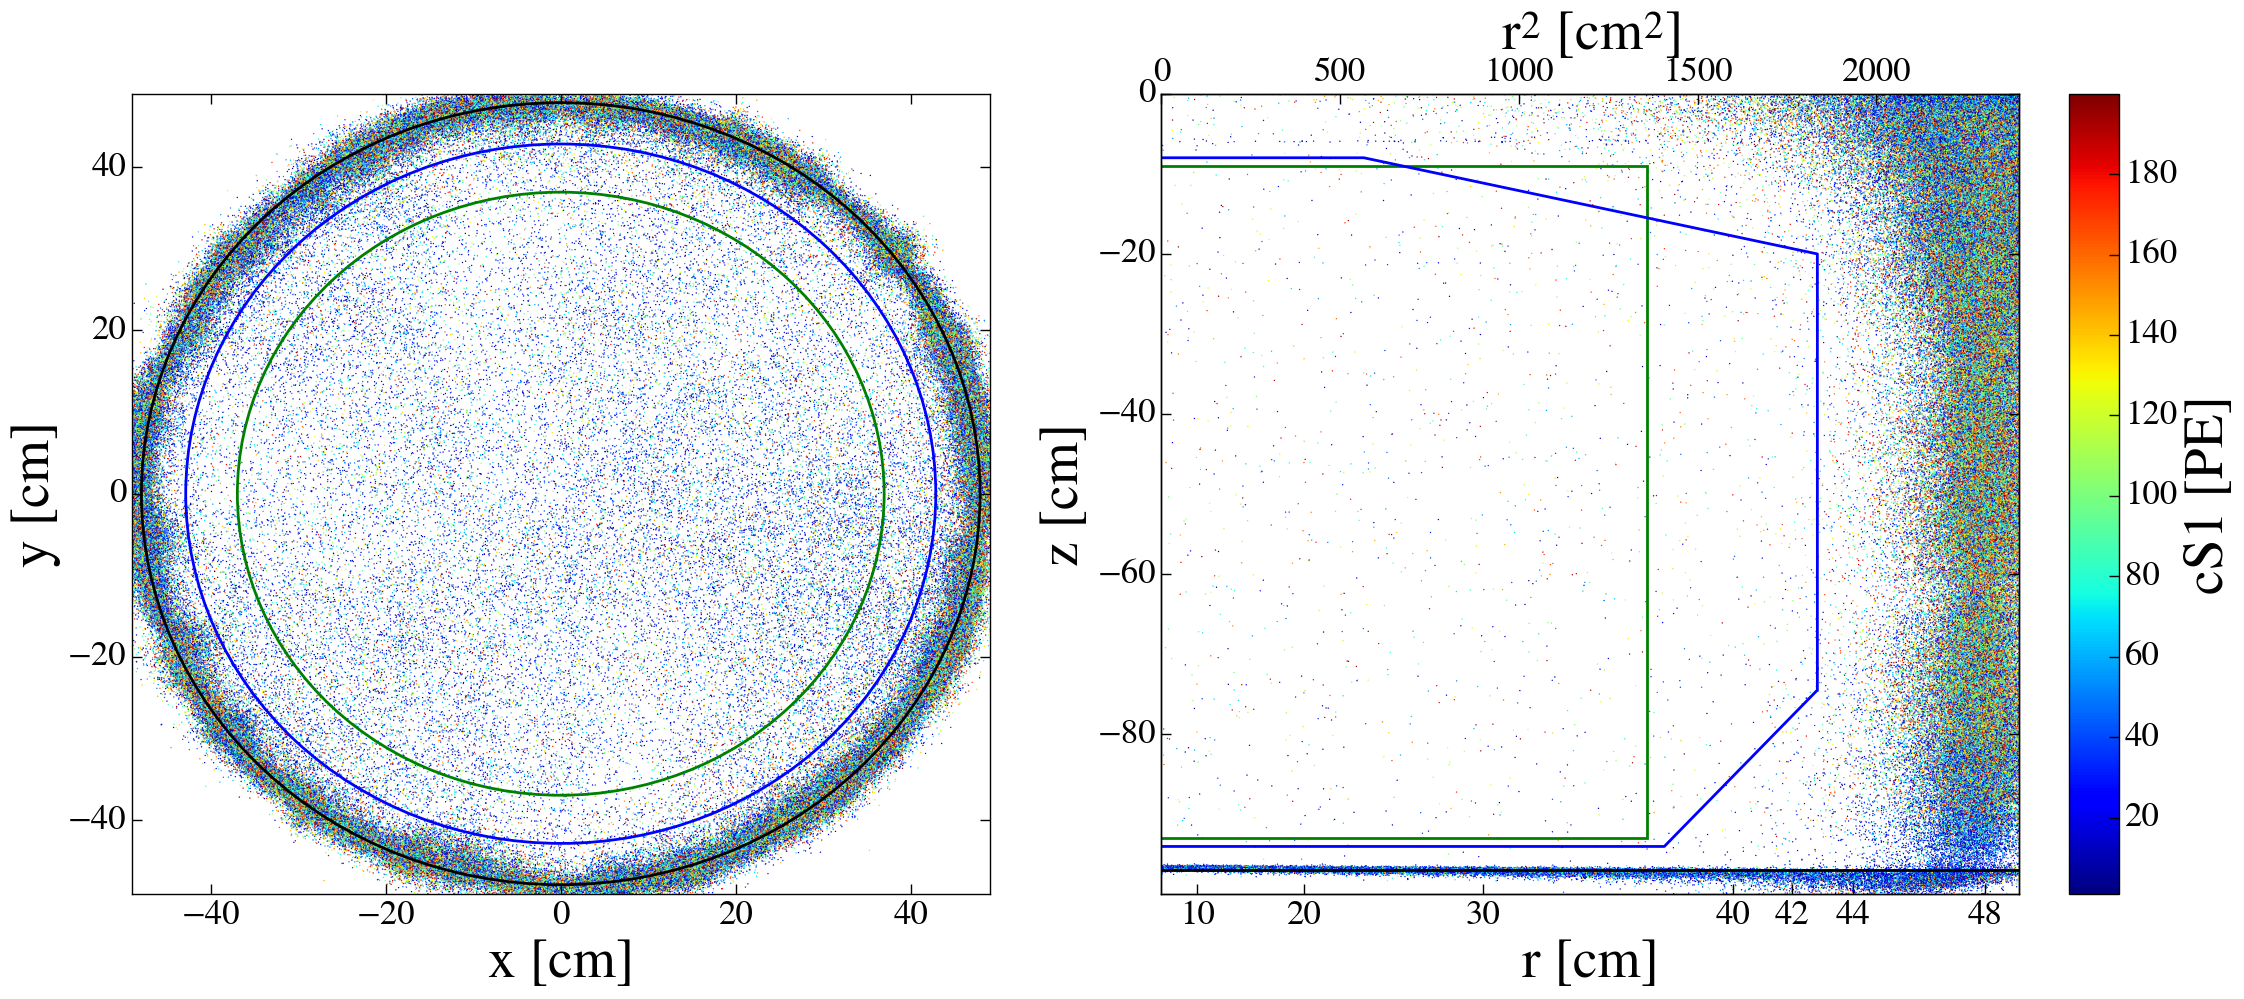
\includegraphics[width=\textwidth]{FVBoth}
\caption{Positions of background events plotted in $x$ vs. $y$ and $r$ ($r^2$) vs. $z$ for SR1.  The 1 ton FV originally used
in SR0 is shown in green and defined by $-92.9 < z < -9\ \mathrm{cm}$, $r < 36.94\ \mathrm{cm}$.  The 1.3 ton FV for SR1 is outlined in
blue, with the maximum radius plotted in the left panel.  Its shape is more complicated but has $z_\mathrm{min} = -94\ \mathrm{cm}$,
$z_{\mathrm{max}} = -8\ \mathrm{cm}$, and $r_{\mathrm{max}} = 42.84\ \mathrm{cm}$.  The active volume (surrounded by the cathode, wall,
and gate) is marked in black.  The events that appear outside the wall are wall events that were not properly
reconstructed.  The events below the cathode result from field inhomogeneities that lead to extended drift times, which is why they
become more exaggerated towards the bottom corner of the TPC.}
\label{fig:calibrations_position_reconstruction}
\end{figure}



\subsection{Electron Lifetime}
\label{subsec:det_char_elifetime}
The electron lifetime $\tau_e$ (see \secref{subsec:tpcs_working_principle} for impurity attachment details) quantifies the charge $q$ that
is lost as it drifts to the liquid-gas interface.  It is given by

\begin{equation}
q(t_d) = q_0 e^{-t_d / \tau_e}
\end{equation}

where $q_0$ is the charge that escapes recombination.  Calibrations with mono-energetic interactions are an excellent method of
measuring $\tau_e$.  The large number of statistics means it can be measured with much higher precision than the
nominal method of using the low-rate background \ce{^{222}Rn} and \ce{^{218}Po} $\alpha$-decays.

The 41.5 keV $\mathrm{^{83m}Kr}$ de-excitation offers a relatively low-energy electronic recoil to measure $\tau_e$.  The number of events
from a typical calibration of 2-3 days is in the millions and any background is negligible.  The left panel of
\figref{fig:calibrations_elifetime_kr} shows a standard electron lifetime calculated using $\mathrm{^{83m}Kr}$.

\begin{figure}
\centering
\includegraphics[width=\textwidth]{S1S2}
\label{fig:calibrations_kr_s1_s2}
\end{figure}

\begin{figure}
    \centering
    \begin{subfigure}[t]{0.45\textwidth}
        \centering
        \includegraphics[width=\textwidth]{KrElectronLifetime}
    \end{subfigure}%
    \begin{subfigure}[t]{0.45\textwidth}
        \centering
        \includegraphics[width=\textwidth]{Bi212ElectronLifetime}
    \end{subfigure}
    \caption{}
	\label{fig:calibrations_elifetime}
\end{figure}

Another high-statistic calibration used for measurement is \ce{^{220}Rn}.  Primarily used for the 569.9 keV $\beta$-emission of its
decay chain daughter \ce{^{212}Pb} (\secref{subsubsec:er_nr_calibrations_parameter_determ_er}), a number of elements along the chain
undergo $\alpha$-decays that can be
used.  \tabref{tab:alpha_decays} lists the main $\alpha$-emitters in both the \ce{^{222}Rn} and \ce{^{220}Rn} chains.  Because calibration
data is only used after the source valve is closed, the 55.6 s and 145 ms half-lives of the first two $\alpha$-emitters \ce{^{220}Rn} and
\ce{^{218}Po}, respectively cannot be used.  However \ce{^{212}Bi} releases a 6.207 MeV $\alpha$ in its decay to \ce{^{208}Tl} with a
branching ratio of 36.9\%.  A typical electron lifetime is shown in the right panel of \figref{fig:calibrations_elifetime}.

Other sources can be used for measuring $\tau_e$ but with less success.  In past experiments the 661.7 \gammaray of \ce{^{137}Cs} was
used, but an early trial in XENON1T showed that very few actually reached the active volume, making the method inefficient.  Additionally
the 163.9 and 236.1 keV de-excitations of $\mathrm{^{131m}Xe}$ and $\mathrm{^{129m}Xe}$, respectively, following a nuclear recoil calibration are
usable initially but longer time windows are required as they de-excite, and they do not offer the large statistics of $\mathrm{^{83m}Kr}$ or
\ce{^{220}Rn}.

\bgroup
\def\arraystretch{1.2}
\begin{table}
\centering
\begin{tabular}{cccccc}
\hline
Isotope & Daughter & Energy & $t_{1/2}$ & Chain \\
\hline
\ce{^{222}Rn} & \ce{^{218}Po} & 5.590 MeV & 3.82 d & \ce{^{222}Rn} \\
\ce{^{218}Po} & \ce{^{214}Pb} & 6.115 MeV & 3.10 m & \ce{^{222}Rn} \\
\ce{^{214}Po} & \ce{^{210}Pb} & 7.833 MeV & $164.3\ \mathrm{\mu s}$ & \ce{^{222}Rn} \\
\ce{^{210}Po} & \ce{^{206}Pb} & 5.407 MeV & 138.4 d & \ce{^{222}Rn} \\
\ce{^{220}Rn} & \ce{^{216}Po} & 6.405 MeV & 55.6 s & \ce{^{220}Rn} \\
\ce{^{216}Po} & \ce{^{212}Pb} & 6.906 MeV & 145 ms & \ce{^{220}Rn} & \\
\ce{^{212}Bi} & \ce{^{208}Tl} & 6.207 MeV & 1.01 d & \ce{^{220}Rn} & \\
\ce{^{212}Po} & \ce{^{208}Pb} & 8.954 MeV & 299 ns & \ce{^{220}Rn} & \\
\hline
\end{tabular}
\caption{$\alpha$-decays with high likelihoods for \ce{^{222}Rn} and \ce{^{220}Rn} decay chains.  \ce{^{222}Rn} makes up part of our
background so it an \ce{^{218}Po} are used to continually monitor the $\tau_e$.  The \ce{^{220}Rn} content in our background is
insignificant but it is used in calibrations, where \ce{^{212}Bi} allows high-statistic measurement.  Those with negligible probability
(\ce{^{218}At}, \ce{^{218}Rn}, \ce{^{214}Bi}, \ce{^{210}Bi}, \ce{^{210}Pb}, \ce{^{209}Pb} for \ce{^{222}Rn} chain, \ce{^{220}Ra} and
\ce{^{216}Rn} for \ce{^{220}Rn} chain) are not listed.}
\label{tab:alpha_decays}
\end{table}
\egroup



\subsection{Single Electron Gain}
\label{subsec:det_char_single_electron_gain}
In measuring the S2 we know the total number of photoelectrons freed from the photocathodes of the PMTs.  However, our parameter of
interest is the number of \electron that were extracted across the GXe.  To convert between the two we need to measure the number of
detected photons per $e^-$, also known as the \textit{single electron gain}, or \textit{gas gain}, $G_e$.  To do so we look at the
smallest features in the waveforms of events that have the width of an S2, and therefore must be single $e^-$.  These generally result
from photoionization of detector metals such as the gate or cathode, photoionization of impurities in the LXe, and delayed extraction
of \electron from the liquid.

The number of photons emitted depends on - among other things - the electric field between the anode and gate $E_g$.  Details of the
exact relation can be found in \secref{subsec:tpcs_working_principle} and \eqref{eq:electronlum}.  The sagging - although small - of the
anode changes $E_g$ slightly along $r$ as mentioned in \secref{subsec:det_char_s2_position_correction} and shown in
\figref{fig:calibrations_s2_maps} (top).  Additionally the dielectric constant of LXe and GXe are different, so a change in liquid level
would cause a nonuniform shift in field, so is monitored over the course of data taking.

Poisson processes give a good approximation to both $G_e$ and the number of photons detected by the PMTs.  Effects like variation in $E_g$
and PMT detection efficiencies apply a smearing.  If this is taken to be Gaussian the number of photons detected is represented by a
Poisson distribution convolved with a Gaussian.  \figref{fig:calibrations_single_electron_gain_num_photons} shows the distribution of
the gas gain for a PMT in SR1.  The spectrum is given in hits, where a hit is defined as the PMT voltage surpassing its assigned threshold
inside the time window that defines the event.

\begin{figure}
\centering
\includegraphics[width=\textwidth]{GasGainImage}
\label{fig:calibrations_single_electron_gain_num_photons}
\end{figure}



\subsection{Average Photon Detection and Charge Extraction Efficiencies}
\label{subsec:det_char_photon_charge_efficiencies}
Applying the above corrections leads to $\mathrm{S1} \rightarrow \mathrm{cS1}$ and $\mathrm{S2} \rightarrow \mathrm{cS2}$ where cS1 and
cS2 are the corrected S1 and S2.  An event of the same energy at the same electric field will result in a cS1 and cS2 independent of
detector effects.  For XENON1T we ignore the top PMT array for S2s.  To differentiate \stwob and \cstwob are used to represent the portion
of the S2 and cS2 observed by the bottom array.  Everything that follows in this chapter uses \stwob and $\mathrm{cS2_b}$.  The processes
for light and charge production were described in \secref{sec:scintillation}.  For electronic recoils atomic motion is
not a factor so all of the energy produces a number of quanta $n_q = E_{er} / W$ where $E_{er}$ is the ER energy and
$W = 13.7 \pm 0.2\ \mathrm{eV}$ is the average energy to create an exciton or electron-ion pair.  The number of quanta can be broken
down as

\begin{equation}
n_q = n_{\gamma} + n_e
\end{equation}

\noindent where $n_{\gamma}$ are $n_e$ are the number of photons and \electron produced, respectively.  This can be rewritten in terms of
observables as

\begin{equation}
\frac{E_{er}}{W} = \frac{\mathrm{cS1}}{g1} + \frac{\mathrm{cS2_b}}{\eta G_e}
\label{eq:calibrations_s1_s2}
\end{equation}

\noindent where $n_{\gamma} = \mathrm{cS1} / g1$ and $n_e = \mathrm{cS2_b} / \eta G_e$ (here we now take $G_e$ to be the single electron
gain as measured by the bottom PMT array) where $g1$ is the average light collection
efficiency and $\eta$
is the \textit{extraction efficiency} - that is, the probability of extracting an \electron from the liquid into the gas.  The average
gain for an \electron then that escapes recombination is $g2 = \eta G_e$.  If $G_e$ is known
(\secref{subsec:det_char_single_electron_gain}) there energy of an event is known \eqref{eq:calibrations_s1_s2} has two unknowns:
$g1$ and $\eta$ (or $g2$).  Rearranging gives

\begin{equation}
\frac{\mathrm{cS2_b}}{E_{er}} = \frac{\eta G_e}{g1} \frac{\mathrm{cS1}}{E_{er}} - \frac{\eta G_e}{W}
\end{equation}

\noindent that shows these can be solved using a linear fit if more than one energies are
used.  \figref{fig:calibrations_photon_charge_efficiencies_g1_g2} (left) presents this for several lines in our detector during SR1, giving
$g1 = 0.1426 \pm 0.0001_{\mathrm{stat}} \pm 0.0017_{\mathrm{sys}}\ \mathrm{PE/ph}$ and $\eta = $
($g2 = 11.55 \pm 0.01_{\mathrm{stat}} \pm 0.24_{\mathrm{sys}}\ \mathrm{PE/e^-}$).  If we account for the emission of two photoelectrons by
a single photon with probability $p_{\mathrm{dpe}} = 0.18-0.24$ (\citeref{Faham2015}) the
photon detection efficiency becomes $g1 = $.  Because $g1$ depends on the PMTs, $\eta$ on the anode-gate electric field, and $G_e$ on
$E_g$, $P$, and distance between the gate and anode they are independent of the drift field.  $g1$ and $g2$ were monitored over the
course of SR1 to ensure any variations are noted.  \figref{fig:calibrations_photon_charge_efficiences_g1_g2} (right) shows that both
were stable.

\begin{figure}
    \centering
    \begin{subfigure}[t]{0.45\textwidth}
        \centering
        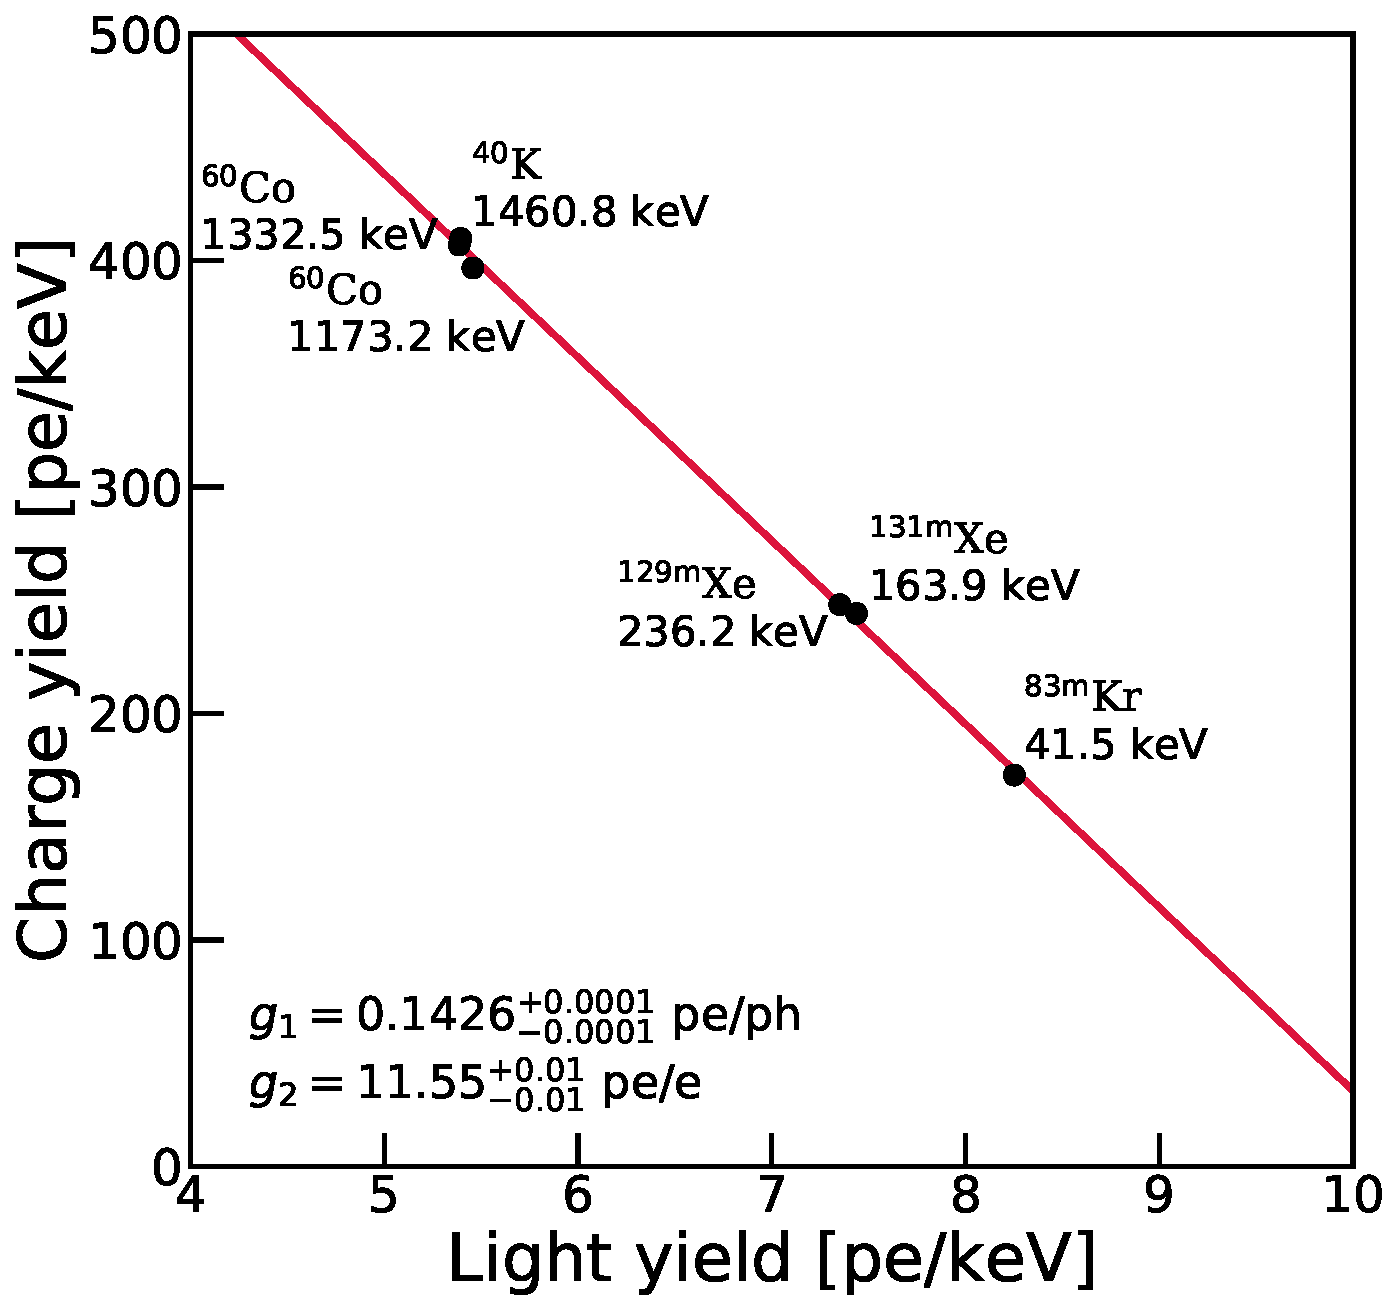
\includegraphics[width=\textwidth]{g1g2Anticorrelation}
    \end{subfigure}%
    \begin{subfigure}[t]{0.45\textwidth}
        \centering
        \includegraphics[width=\textwidth]{TimeDependence}
    \end{subfigure}
    \caption{}
	\label{fig:calibrations_photon_charge_efficiences_g1_g2}
\end{figure}

Returning to \eqref{eq:calibrations_s1_s2} we see after solving for $g1/\eta/g2$ we can reconstruct $E$ for any ER event.  The (ER)
background is shown in \figref{fig:calibrations_photon_charge_efficiences_ces} for the 1 t fiducial volume during SR1.  Key peaks are
labeled with their respective energy and responsible isotope.  We can see that during DM data taking some $\mathrm{^{83m}Kr}$ is present, most
likely from \ce{^{83}Rb} initially absorbed in the getters but some time later decay.  $\mathrm{^{129m}Xe}$ and $\mathrm{^{131m}Xe}$ are clearly
visible though the majority of their de-excitations occur in the weeks following the AmBe and the NG.  Other well-defined features
include \ce{^{214}Bi} (609.3, 1764.5, and 2204.1 keV), \ce{^{60}Co} (1173.2 and 1332.5 keV), \ce{^{40}K} (1460.8 keV), and \ce{^{208}Tl}
(2614.5 keV).  They sit on a continuous energy spectrum caused by $\gamma$-rays that deposit part of their energy before leaving the
detector, $\beta$-decays, and the $2 \nu \beta \beta$ emission of \ce{^{136}Xe}.

The energy resolution is a measure of how well different energy depositions can be distinguished from one another.  Better resolution
allows differentiation of nearby energy features, which allows improved discrimination between signal and background.  It is calculated
by fitting a mono-energetic \gammaray line with a gaussian and dividing the width by the mean.  This is done for a number of background
lines as shown in \figref{fig:calibrations_photon_charge_efficiences_ces_resolution}.  Our energy resolution improves at higher energies
as $\sigma / E = (27.30 \pm 0.37) / \sqrt{E} + (0.65 \pm 0.03)$ including high energy (> 1.5 MeV) lines and
$\sigma / E = (30.98 \pm 0.43) / \sqrt{E} + (0.37 \pm 0.03)$ without.  The second term refers to the fundamental limit of the
resolution.  We can see our energy resolution is better than XENON100, PandaX, and LUX.

\begin{figure}
\centering
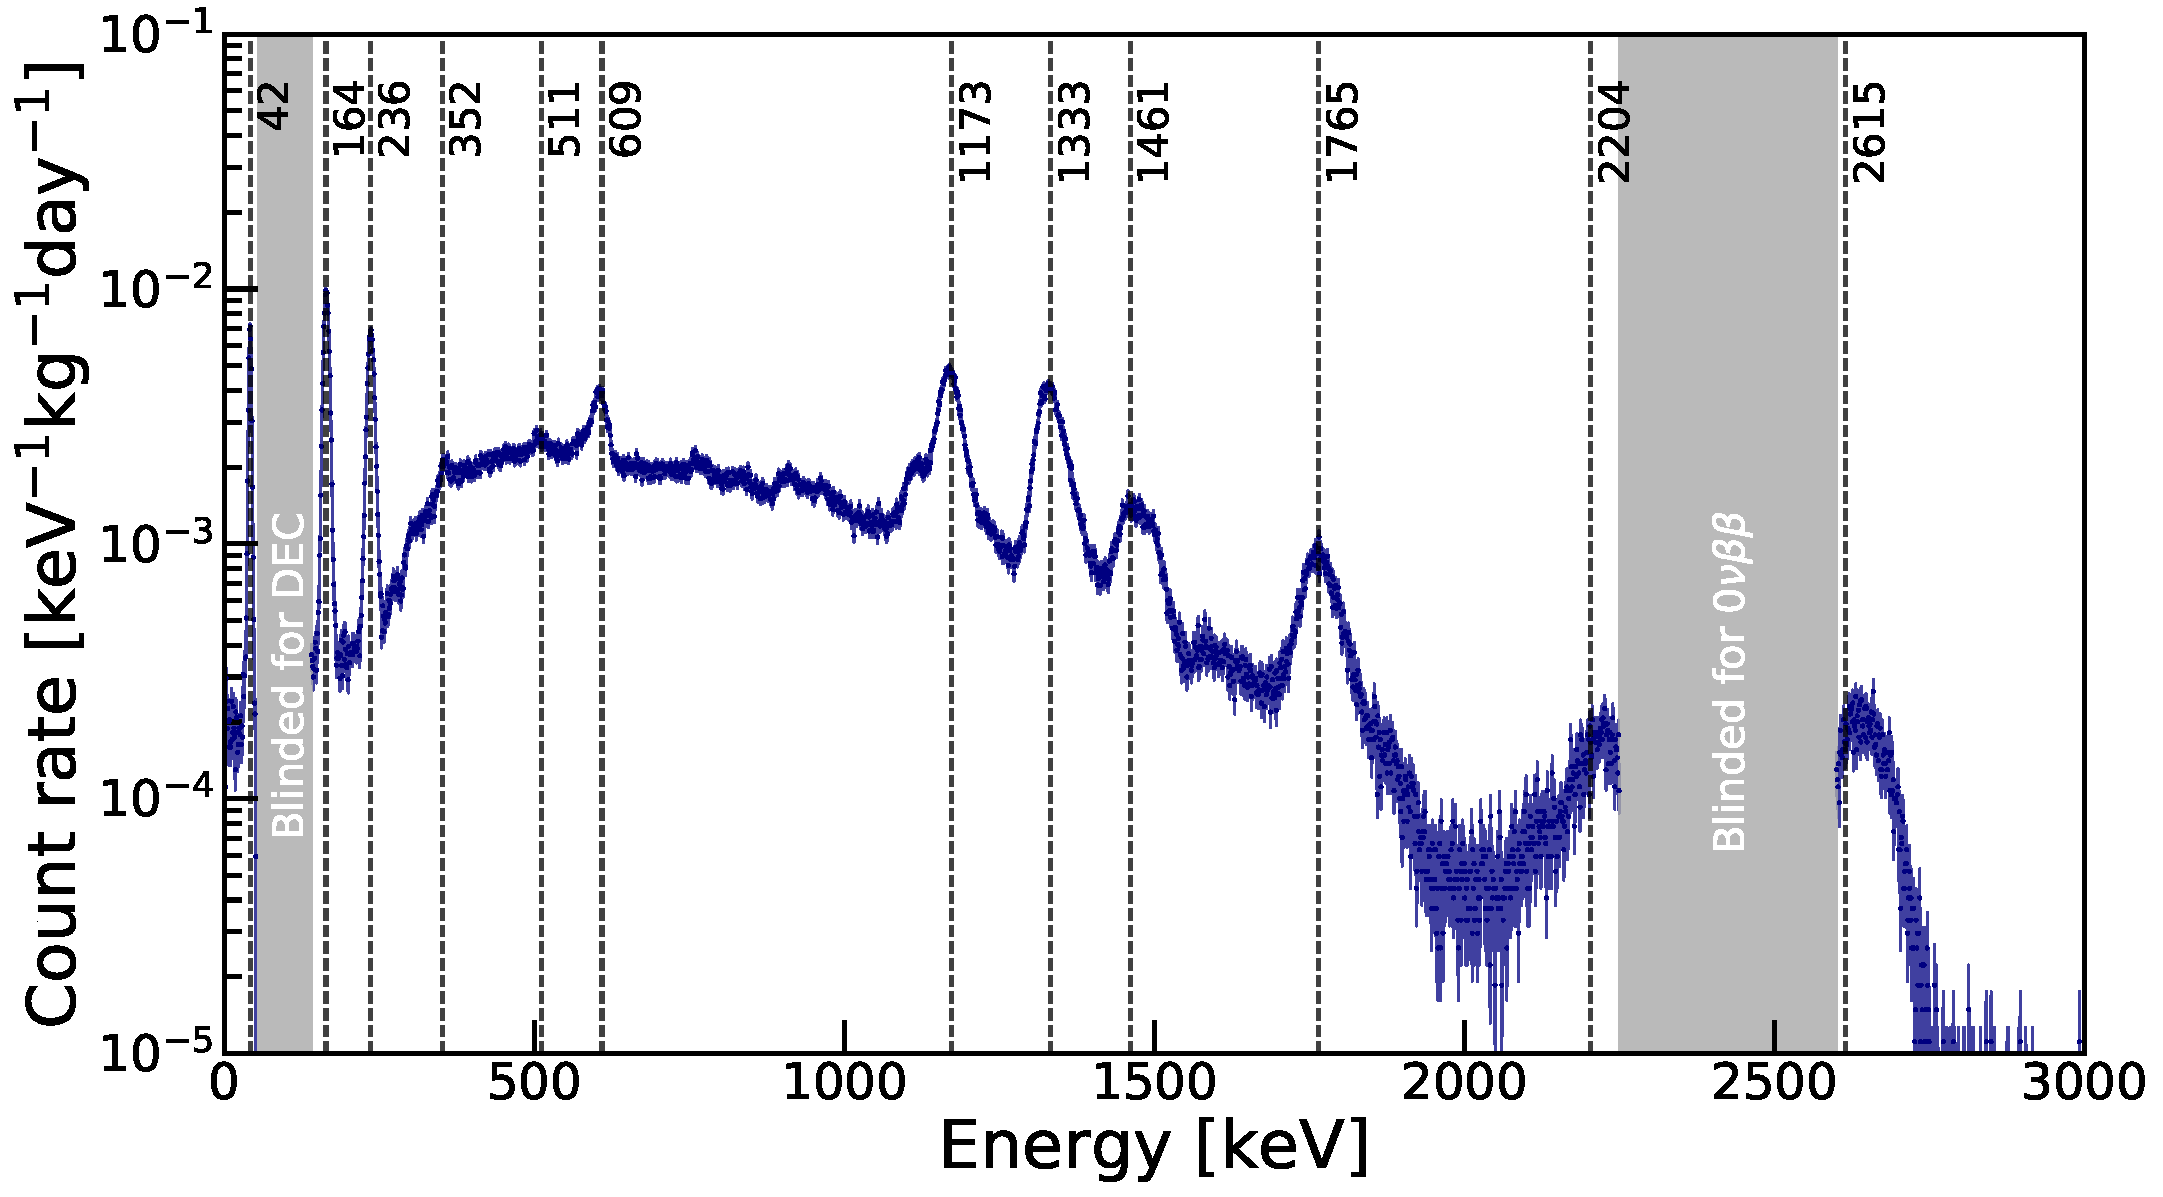
\includegraphics[width=\textwidth]{EnergySpectrum}
\label{fig:calibrations_photon_charge_efficiencies_ces}
\end{figure}

\begin{figure}
\centering
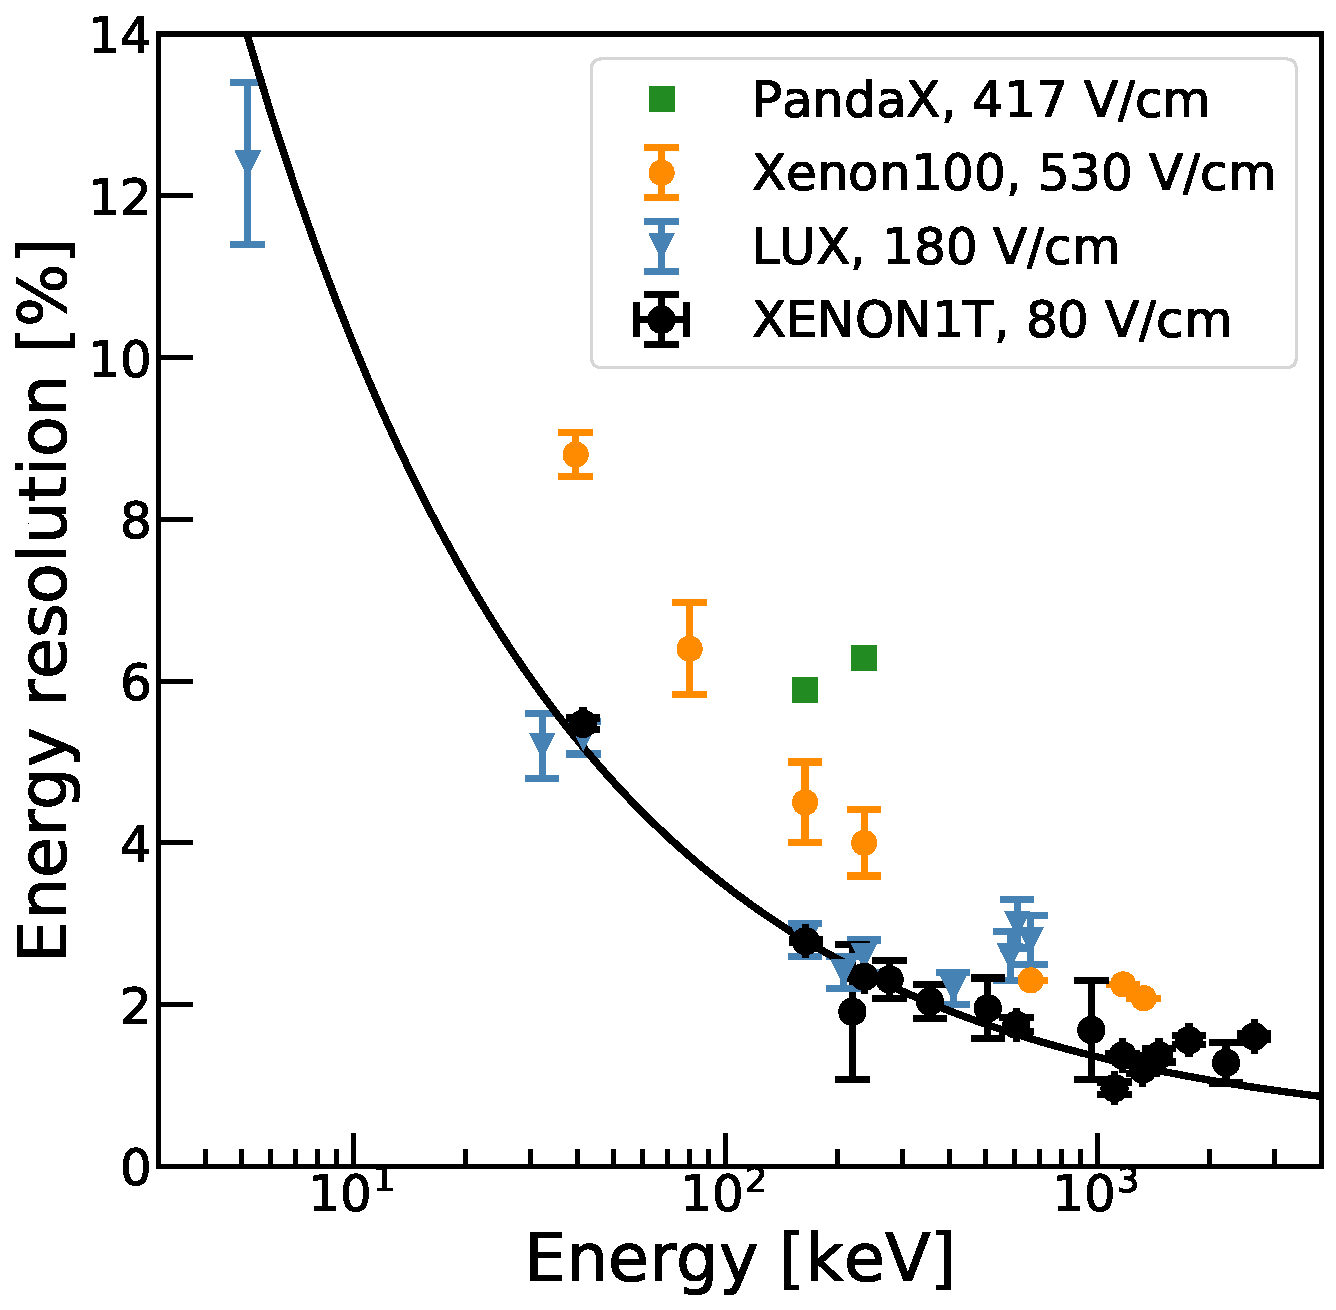
\includegraphics[width=0.8\textwidth]{EnergyResolution}
\label{fig:calibrations_photon_charge_efficiences_ces_resolution}
\end{figure}



\subsection{Bias and Smearing}
\label{subsec:det_char_bias_smearing}



\section{Electronic and Nuclear Recoil Bands}
\label{subsec:er_nr_calibrations}
To differentiate our nuclear from electronic recoil bands we need to calibrate each independently.  While the detector characterizations
discussed in \secref{sec:det_char} lead to improved accuracy and precision or are in some cases very important, these are critical as
they allow discrimination between at potential WIMP and ER background.  As mentioned in
\secref{subsec:det_char_elifetime} \ce{^{220}Rn} is used for our ER band.  For NR we use \ce{^{241}AmBe} and a neutron generator (NG),
each of which are positioned in the water tank outside the cryostat.

Science Run 1 marks the first time the electronic and nuclear recoil bands were fit simultaneously (for SR0 they were independent).  This
is significant because shared detector parameters (e.g. $W$, $g1$, $g2$, $p_{\mathrm{dpe}}$, etc.) are constrained to a single value
across calibrations.  Using the physical processes from the interaction itself to the final values of cS1 and \cstwob in the fit is made
possible by running on GPUs, which provide a $10^{2 \mdash 3}$ times speed increase.



\subsection{Purpose of Calibrations}
\label{subsec:er_nr_calibrations_purpose}
The electronic and nuclear recoil calibrations are important because they create a probability density function (PDF)
such that for any event we can quantify the likelihood of what caused it.  This provides dramatically improved sensitivity
to purely statistical approaches (\secref{sec:direct_detect}).  Doing so requires a complete understanding of the TPC background, which
in addition to nominal electronic recoils includes accidental coincidence (AC) and wall leakage events \secref{}.  It also demands that
the physical processes that occur starting from the exciton-ion ratio through the data acquisition are correctly modeled and able to be
simulated on a reasonable time scale.

Following the ER and NR fits a signal PDF is generated.  For our DM search the
signal is a WIMP but in general it is not constrained to this.  The shape of the PDF depends on the WIMP mass.  The data can be compared
to the PDF for a given WIMP mass and cross-section to see whether it agrees with a signal.  A limit is set if all cross-sections below
some value match the data, while a discovery can be claimed if the data prefers a particular mass and cross-section over others.

\figref{fig:er_nr_calibrations_wimp_contours} shows the background model with contours for a 50 GeV WIMP overlaid.  The ER band is clearly
present and we can see the overlap between the two, which exemplifies the necessity of lowering the overall background for improved
sensitivity.

\begin{figure}
\centering
\includegraphics[width=\textwidth]{WIMPContours}
\caption{Some on SR0 blessed plots page}
\label{fig:er_nr_calibrations_wimp_contours}
\end{figure}

The fits are performed using a Markov Chain Monte Carlo (\citeref{Foreman-Mackey}).



\subsection{Parameter Determination}
\label{subsec:er_nr_calibrations_parameter_determ}
This approach compares the distribution of Monte Carlo events with the data.  Because of the nearly flat distribution of events at relevant
energies along with homogenous distribution, Monte Carlo features $E$, $x$, $y$, $z$, for \ce{^{220}Rn} are randomly sampled from a
uniform distribution.  \ce{^{241}AmBe} and neutron generator Monte Carlo are generated using GEANT4, and also include the number of
scatters for each neutron.  The $\beta$ from \ce{^{220}Rn} should not scatter so this is fixed to 1.  These represent the ``truth''
information - that is, these are the true interaction values.

\figref{fig:er_nr_calibrations_parameter_determ_flow_chart} shows the flow chart for the band matching.  Each Monte Carlo event is run
through a series of events that mimic the true sequence as closely as possible.  The parameters used in this estimation come from
a variety of sources including physical properties reported from literature and detector characterization measurements
(\secref{sec:det_char}).  The process takes the simulated energy from a Monte Carlo event and ultimately outputs observables cS1 and
$\mathrm{cS2_b}$.  These in turn are binned in cS1 vs. $\mathrm{log_{10}(cS2_b / cS1)}$ space, and the likelihood for equivalent bins
between data and MC is calculated (discussed in \secref{subsec:er_nr_calibrations_likelihood}).  As the parameters vary the likelihood
should increase or decrease, allowing a minimizer to find the best-fit values.  An important consideration is the penalty terms from the
priors are included in the likelihood so the simulated PDF is constrained.

\begin{figure}
\centering
\includegraphics[width=\textwidth]{FlowChart}
\label{fig:er_nr_calibrations_parameter_determ_flow_chart}
\end{figure}

The number of events simulated for each likelihood iteration is $\mathcal{O}(10^6)$.  Such large statistics are necessary for convergence;
however, nominal running time is far greater than any sensible time-scale.  This was solved by using graphical processing units (GPUs),
which can run the events in parallel, providing a boost in speed is $10^{2 \mdash 3}$ times and reducing the required time to a
reasonable level.

The author will refer to the conversion of truth MC to cS1 and \cstwob as a ``fast MC'' (the parameters used in each event are pulled
from a random number generator).  ``Truth MC'' will refer to the simulated events before the fast MC (actual $E$, $x$, $y$, $z$, and number
of scatters as described above).  ``MC'' will denote the sum of all the fast MC components, usually in the form of a PDF (histogram), for
a single data-MC comparison.  Finally, a Markov Chain Monte Carlo (MCMC) is used to fit the data and Monte Carlo.  The best-fit values
then are derived from the posterior.  \secref{subsubsec:er_nr_calibrations_parameter_determ_er} (ER) and
\secref{subsubsec:er_nr_calibrations_parameter_determ_nr} (NR) discusses the physical steps that occur beginning with a single energy
deposition until final cS1 and $\mathrm{cS2_b}$ (and by extension the operations applied in the fast MC).

The calibrations were fit in the SR0 FV ($-92.9 < z < -9\ mathrm{cm}$, $r < 36.94\ \mathrm{cm}$
\figref{fig:calibrations_position_reconstruction}) despite it being different from SR1.  This was done to minimize wall events as well as
contamination from materials at the top and bottom of the TPC (mainly PMTs).



\subsubsection{Electronic Recoils}
\label{subsubsec:er_nr_calibrations_parameter_determ_er}
The electronic recoil calibration is performed using \ce{^{220}Rn} (decay chain shown in the left panel of
\figref{fig:backgrounds_decay_chains}).  It is used because of the \ce{^{212}Pb} \betadecay with Q-value 569.9 keV and can be performed
as an internal calibration.  T

When energy is deposited in the LXe a number of quanta will be produced.  For electronic recoils this follows the normal distribution

\begin{equation}
n_q \sim \mathrm{N} \bigg( \mu = \frac{E}{W},\ \sigma^2 = \frac{E F}{W} \bigg)
\end{equation}

\noindent where $F$ is the Fano Factor (\citeref{Fano1947}) introduced in \secref{sec:er}.  Its derivation and subsequent measurements
demonstrates
that fluctuations in $n_q$ are smaller than a Poisson distribution, and is estimated to be $F = 0.059$ (\citeref{Doke1976}).  For the
fast MC $F$ is held fixed, although it should be noted that a later measurement found different best-fit values, though their result was
compatible with \citeref{Doke1976} when including uncertainty (\citeref{Seguinot1995}).  $W$, the average energy to produce a single
quanta, is constrained by a Gaussian with $\mu = 13.7,\ \sigma = 0.2\ \mathrm{eV}$ following the measurement of \citeref{Dahl2009}.

For ER any quenching is considered negligible so is not considered.  The quanta will be divided into excitons and electron-ion pairs
$n_q = n_{\mathrm{ex}} + n_{\mathrm{ion}}$ and will be divided according to a binomial distribution

\begin{equation}
n_{\mathrm{ion}} \sim \mathrm{Binom} \Bigg(n = n_{\mathrm{q}},\ p = \frac{1}{1 + \frac{n_{\mathrm{ex}}}{n_{\mathrm{ion}}}} \Bigg)
\label{eq:er_nr_calibrations_parameter_determ_er_nions}
\end{equation}

\noindent where $n_{\mathrm{ex}} / n_{\mathrm{ion}}$ is between 0.06-0.2 and expected to be independent of energy
(\citeref{NEST2011}).  Next we must consider the recombination fraction $r$ where some \electron will reattach to a \ce{Xe^+} to form
excitons and upon decay to their ground state emit photons.  $r$ depends on the field in the LXe and the interaction energy, and has
intrinsic fluctuation $\delta r$ that cannot be ignored (\citeref{LUX2016, Aprile2017e}).  We assume a truncated Gaussian

\begin{equation}
r \sim \mathrm{N} \Big( \mu = \langle r \rangle,\ \sigma^2 = (\delta r)^2 Big)
\end{equation}

\noindent where $r = 0 \mdash 1$ and is parameterized as a fourth order polynomial with some energy threshold
$E_{\mathrm{thresh}}$ such that if $E < E_{\mathrm{thresh}},\ r = 0$.  Recombination fluctuations are defined as
$\delta r = A(1 - e^{E/B})$.  All eight parameters (five from polynomial, one from $E_{\mathrm{thresh}}$, two from $\delta r$) are allowed
to vary freely (with no penalty term in likelihood) though $A,B > 0$.  The number of electron-ion pairs that recombine is

\begin{equation}
n_{\mathrm{rec}} \sim \mathrm{Binom} \Big(n = n_{\mathrm{ion}},\ p = r \Big)
\end{equation}

\noindent yielding a final number of photons and electrons

\begin{equation}
\begin{aligned}
n_{\mathrm{ph}} = n_{\mathrm{ex}} + r n_{\mathrm{rec}} \\
n_{\mathrm{e}} = (1 - r) n_{\mathrm{rec}}
\end{aligned}
\end{equation}

\noindent  As mentioned above \ce{^{220}Rn} is homogeneously spread throughout the TPC and has an energy spectrum that is nearly flat
between 0-30 keV so its truth MC values ($E$, $x$, $y$, and $z$) were each randomly sampled from a uniform distribution.



\begin{Nuclear Recoils}
\label{subsubsec:er_nr_calibrations_parameter_determ_nr}
Two nuclear recoil sources were used for calibrations: americium beryllium (\ambe) and a neutron generator (NG).  \ambe decays to
\ce{^{237}Np} through $\alpha$-emission where the large \ce{^{9}Be} $\alpha$ cross-section prompts a second decay via

\begin{equation}
\mathrm{^{9}Be} + \mathrm{^{4}He} \rightarrow \mathrm{^{12}C + n} + \gamma
\end{equation}

\noindent emitting a $< 11\ \mathrm{MeV}$ neutron.  The neutron generator (NSD Gradel Fusion NSD-35-DD-C-W-S) uses
deuterium-deuterium (DD) fusion

\begin{equation}
\mathrm{^{2}D} + \mathrm{^{2}D} \rightarrow \mathrm{^{3}He} + \mathrm{n}
\end{equation}

\noindent where the \ce{^{3}He} and n are expelled at 0.82 and 2.45 MeV, respectively.  The energy spectrum can be seen in
\figref{fig:er_nr_calibrations_parameter_determ_nr_ng_energy}.  It shows two peaks - one at 2.2 MeV and the other at 2.7 MeV.  These
are the energies as seen in the lab frame (2.45 MeV was in the deuteron's) and correspond to neutrons emitted at $180^{\circ}$ and
$0^{\circ}$, respectively.  The NG can operate at rates as low as $10\ \mathrm{n\ s^{-1}}$
and as high as $10^7\ \mathrm{n\ s^{-1}}$, which allows more flexibility in our objectives.  A higher-energy neutron
population is produced by tritium via

\begin{figure}
\centering
\includegraphics[width=0.6\textwidth]{Fig5Lang2018}
\caption{Image credit: \citeref{Lang2018}.}
\label{fig:er_nr_calibrations_parameter_determ_nr_ng_energy}
\end{figure}

\begin{equation}
\begin{aligned}
\mathrm{^{2}D} + \mathrm{^{2}D} \rightarrow \mathrm{^{3}T} + \mathrm{p} \\
\mathrm{^{3}T} + \mathrm{^{2}D} \rightarrow \mathrm{^{4}He} + \mathrm{n}
\end{aligned}
\end{equation}

\noindent that expels neutrons at 14.1 MeV.  The contribution of deuterium-tritium fusion was measured to be $3.5 \pm 0.2\%$ before
installation at LNGS (\citeref{Lang2018}).  Because the tritium is created in deuterium-deuterium fusion and has
$t_{1/2} = 1.3\ \mathrm{y}$ this fraction is expected to increase with continued use.  For details on the characterization of the NG
please refer to \citeref{Lang2018}.

The energies and positions for \ambe and the NG are shown in \figref{fig:er_nr_calibrations_parameter_determ_nr_ambe_spectrum}.  The
interactions are clustered near a particular $\phi$ that corresponds to the location of the calibration source.  However, we expect our
detector does not vary along $\phi$ so the lopsided position distribution can be applied to the entire active volume.

\begin{figure}
    \centering
    \begin{subfigure}[t]{0.45\textwidth}
        \centering
        \includegraphics[width=\textwidth]{AmBeEnergy}
    \end{subfigure}%
    \begin{subfigure}[t]{0.45\textwidth}
        \centering
        \includegraphics[width=\textwidth]{AmBePositions}
    \end{subfigure}
    \vskip\baselineskip
    \begin{subfigure}[t]{0.45\textwidth}
        \centering
        \includegraphics[width=\textwidth]{NGEnergy}
    \end{subfigure}%
    \begin{subfigure}[t]{0.45\textwidth}
        \centering
        \includegraphics[width=\textwidth]{NGPositions}
    \end{subfigure}
    \caption{}
	\label{fig:er_nr_calibrations_parameter_determ_nr_ambe_spectrum}
\end{figure}

The processes that follow a nuclear recoil differ quite a bit from ER (\secref{subsubsec:er_nr_calibrations_parameter_determ_er}).  As
discussed in \secref{sec:nr} a sizable portion of the energy is lost to atomic motion.  To model this we use the Lindhard theory
as shown in \eqref{eq:er_nr_calibrations_parameter_determ_nr_lindhard}.

\begin{equation}
\begin{aligned}
\epsilon = 11.5 Big( \frac{E}{\mathrm{keV}} Z^{-7/3} \Big)
g(\epsilon) = 3 \epsilon^{0.15} + 0.7 \epsilon^{0.6} + \epsilon \\
L(\epsilon) = \frac{k g(\epsilon)}{1 + k g(\epsilon)}
\label{eq:er_nr_calibrations_parameter_determ_nr_lindhard}
\end{aligned}
\end{equation}

Here $k$ represents the proportionality constant between the electronic stopping power and recoiling nucleus velocity.  The Linhard factor
$L$ is the fraction of energy not converted to excitons or electron-ion pairs

\begin{equation}
n_{\mathrm{q}} \sim P \Big( \mu = \frac{E L}{W} \Big)
\end{equation}

\noindent that uses a Poisson distribution as an approximation.  In reality the track structure of nuclear recoils makes the true
distribution more complicated.  From the number of quanta we follow from \eqref{eq:er_nr_calibrations_parameter_determ_er_nions} for
electronic recoils

\begin{equation}
n_{\mathrm{ion}} \sim \mathrm{Binom} \Bigg(n = n_{\mathrm{q}},\ p = \frac{1}{1 + \frac{n_{\mathrm{ex}}}{n_{\mathrm{ion}}}} \Bigg)
\end{equation}

\noindent and $n_{\mathrm{ex}} = n_{\mathrm{q}} - n_{\mathrm{ion}}$.  Recombination is given by

\begin{equation}
n_{\mathrm{rec}} \sim \mathrm{Binom} \Big(n = n_{\mathrm{ion}},\ p = r \Big)
\end{equation}

\noindent but $r$ now is described by the Thomas-Imel model (\citeref{Thomas1987}).

\begin{equation}
r = 1 - \frac{\mathrm{ln} (1 + n_{\mathrm{ion}} \varsigma)}{n_{\mathrm{ion}} \varsigma}
\end{equation}

\noindent where $\varsigma$ is field-dependent.  Unlike ER, no recombination fluctuations have been observed for nuclear recoils so
$\delta r$ is not considered.  We must also consider biexcitonic quenching and the Penning process, both of which decrease
$\mathrm{n_{ph}}$.  The former arises when two
\ce{Xe^{*}} interact to free an $e^-$, which in turn quickly loses its kinetic energy
and recombines with a \ce{Xe^{+}}.  Thus what would have been two photons instead results in one.  The Penning process describes when
two excimers interact and result in an excited and ground state (\citref{Mei2008}).  Both of these depend on the exciton density, which
is proportional to the ionization density and therefore stopping power $dE / dx$.  Both of these processes result in quenching and can be
described by Birks' saturation law, shown in \eqref{eq:er_nr_calibrations_parameter_determ_nr_birks} (\citeref{Birks1951, Birks1964}).

\begin{equation}
f_l = \frac{1}{1 + k_{B}B \frac{dE}{dx}} = \frac{1}{1 + \eta \epsilon^{\lambda}}
\label{eq:er_nr_calibrations_parameter_determ_nr_birks}
\end{equation}

where $k_B$ is Birks' constant (calculated in \citeref{Mei2008} to be $2.015 \times 10^{-3}\ \mathrm{g\ MeV^{-1}\ cm^{-2}}$), $B$ is
the coefficient to the stopping power, and $\eta$ is defined to be their product.  The total quenching due to biexcitonic quenching and
the Penning process is then

\begin{equation}
n_{\mathrm{q}} = B(n = n_{\mathrm{ex}},\ p = f_l)
\end{equation}

\noindent reducing $n_{\mathrm{ex}} \rightarrow n_{\mathrm{ex}} - n_{\mathrm{q}} \rightarrow n_{\mathrm{ex}}$.

For the \ambe and NG calibrations we constrained our nuclear recoil model based on previous measurements of light and charge yield,
instead of performing an independent measurement.  This decision was made to prevent detector effects from compensating for changes
in the liquid xenon response model.  We applied the results from \citeref{NEST2015}, which uses nuclear recoil light and charge yield
measurements between $1 \mdash 300\ \mathrm{keV}$ and electric fields of $0 \mdash 4060\ \mathrm{V\ cm^{-1}}$ to fit the model
detailed in this section.  Although the none of the measurements were made for light and charge yield simultaneously, \citeref{NEST2015}
performed a single fit including all data.

The model is parameterized by setting

\begin{equation}
\frac{n_{\mathrm{ex}}}{n_{\mathrm{ion}}} = \alpha F_{E}^{\zeta} ( 1 - e^{-\beta \epsilon})
\label{eq:er_nr_calibrations_parameter_determ_nr_nex_nion}
\end{equation}

\begin{equation}
\varsigma = \gamma F_{E}^{- \delta}
\label{eq:er_nr_calibrations_parameter_determ_nr_recomb_sigma}
\end{equation}

\noindent where, to differentiate from energy $E$ and the Fano Factor $F$, the electric field is referred to as $F_E$.  Note that
from \eqref{eq:er_nr_calibrations_parameter_determ_nr_nex_nion} $n_{\mathrm{ex}} / n_{\mathrm{ion}}$ has a power dependence on $F_E$,
which is suspected to be caused by geminate recombination: when electrons and parent ions recombine much more quickly than Thomas-Imel
recombination.  In addition $n_{\mathrm{ex}} / n_{\mathrm{ion}}$ depends exponentially on energy such that at higher $E$ a larger fraction
of excitons is favored.

We see in \eqref{eq:er_nr_calibrations_parameter_determ_nr_recomb_sigma} that $\varsigma$ is proportional to a power of $F_E$.  As
mentioned in \secref{subsec:recombination} the Thomas-Imel theory predicts

\begin{equation}
\varsigma = \frac{\alpha^{'}}{4 a^2 u_- F_E}
\end{equation}

\noindent where $\alpha^'$ is a recombination coefficient, $a$ is the dimension of the box, and $u_-$ is the electron mobility.  While
here $\delta = 1$ strictly, Dahl's model predicts $\delta {\sim} 0.1$ (\citeref{Dahl2009}).

\citeref{NEST2015} leaves $k$ (\eqref{er_nr_calibrations_parameter_determ_nr_lindhard}), $\eta$ and $\lambda$
(\eqref{eq:er_nr_calibrations_parameter_determ_nr_birks}), $\alpha$, $\zeta$ and $\beta$
(\eqref{eq:er_nr_calibrations_parameter_determ_nr_nex_nion}), and $\gamma$ and $\delta$
(\eqref{eq:er_nr_calibrations_parameter_determ_nr_recomb_sigma}) as free parameters to fit.  The results are shown in
\tabref{tab:er_nr_calibrations_parameter_determ_nr_nest}.

\bgroup
\def\arraystretch{1.2}
\begin{table}
\centering
\begin{tabular}{cccc}
\hline
Parameter & Best Fit & Equation \\
\hline
$\alpha$ & $1.240_{-0.073}^{+0.079}$ & \eqref{eq:er_nr_calibrations_parameter_determ_nr_birks} \\
$\zeta$ & $4.72_{-0.73}^{+0.88} \times 10^{-2} $ & \eqref{eq:er_nr_calibrations_parameter_determ_nr_birks} \\
$\beta$ & $239_{-8.8}^{+28}$ \eqref{eq:er_nr_calibrations_parameter_determ_nr_birks} \\
$\gamma$ & $1.385_{-0.073}^{+0.058} \times 10^{-2}$ & \eqref{eq:er_nr_calibrations_parameter_determ_nr_nex_nion} \\
$\delta$ & $6.20_{-0.64}^{+0.56} \times 10^{-2}$ & \eqref{eq:er_nr_calibrations_parameter_determ_nr_nex_nion} \\
$k$ & $0.1394_{-0.0026}^{+0.0032}$ & \eqref{er_nr_calibrations_parameter_determ_nr_lindhard} \\
$\eta$ & $3.3_{-0.7}^{+5.3}$ &  \eqref{eq:er_nr_calibrations_parameter_determ_nr_birks} \\
$\lambda$ & $1.14_{-0.09}^{+0.45}$ & \eqref{eq:er_nr_calibrations_parameter_determ_nr_birks} \\
\hline
\end{tabular}
\caption{Best fit values along with 68\% confidence intetervals from the \citeref{NEST2015} analysis to available nuclear recoil light and
charge yields.}
\label{tab:er_nr_calibrations_parameter_determ_nr_nest}
\end{table}
\egroup

For the SR1 NR fit the values listed in \tabref{tab:er_nr_calibrations_parameter_determ_nr_nest} are used as priors.  Each parameter is
constrained by a gaussian with standard deviation equal to the mean of the $+$ and $-$ uncertainties.  In the future these will be
constrained by asymmetric gaussians.













In an electric field $E$ an \electron that is freed but does not recombine with its parent or other ionized atoms will move anti-parallel
to the field at drift velocity $v_{d}$.  For $E \lesssim 100\ \mathrm{V\ cm^{-1}}$ \vd$\propto E$, $100 \lesssim E \lesssim 10^{3-4}$
\vd$\propto E^{1/2}$, and $E \gtrsim 10^{4}$ \vd plateaus at $\sim 3\ \mathrm{mm\ \mu s^{-1}}$ (\citeref{Miller1968}).


As the electron cloud drifts it will diffuse both longitudinally (in the direction of $E$) and transversely (perpendicular to $E$).  The
diffusion coefficients $D_{L}$ and $D_{T}$ are dependent on the electric field with $D_{T}/D_{L} \sim 10$.  The electron spread can
be written as $\sigma_{D_{T}} = \sqrt{D_{T} t_{d}}$ where $t_{d} = d/v_{d}$ is the drift time and $d$ is the drift distance.

Extensive xenon distillation and purification occurs before it is used in a detector.  Nonetheless impurities outgas from detector
material and contaminate the LXe.  Electronegative impurities in particular present a problem since they will attach to a free \electron,
lowering the number that reach the top of the detector and decreasing the secondary scintillation as shown in \eqref{eq:impurity_attach}.

\begin{equation}
e^{-} + S \rightarrow S^{-}
\label{eq:impurity_attach}
\end{equation}

\noindent The amount of \electron captured is dependent on the time in the LXe.  Thus an advantage of larger \efields is a larger
\vd (up to a point) and thus less time in the liquid.  Doping LXe with organic materials such as butane can increase \vd at higher
\efields but they are not used in DM detectors due to difficulty in purifying (\citeref{Yoshino1976}).  By setting the rate at which
electrons are absorbed by impurities $dq/dt = -qk_{S}S$ where $S$ is the impurity concentration and $k_{S}$ is the attachment rate
constant we find

\begin{equation}
q(t) = q_{0}e^{-tk_{S}S} = q_{0}e^{-t/\tau_{e}}
\label{eq:lifetime_equation}
\end{equation}

\noindent where $\tau_{e} = (k_{S}S)^{-1}$ and is known as the electron lifetime.  $k_{S}$ is shown in \figref{fig:attachment_rate} for
O$_{2}$,
N$_{2}$O, and SF$_{6}$.  We see that for N$_{2}$O the attaching rate constant increases with \efield whereas \otwo and SF$_{6}$
decerase.  Typically impurity concentration is given in O$_{2}$-equivalent values - that is, the concentration of \otwo if it was solely
responsible for \electron attachment.  For modeling electron lifetime it turns out that using the \otwo curve in
\figref{fig:attachment_rate} gives a good approximation.  Removing such impurities will be discussed in detail in \secref{}.

\begin{figure}
\includegraphics[width=0.8\textwidth]{AttachmentRate}
\caption{Attaching rate constant $k_{S}$ from \citeref{Bakale1976} for \otwo, N$_{2}$O, and SF$_{6}$ with respect to electric field.  At
larger \efield $k_{S}$ increases for N$_{2}$O and decreases for \otwo and SF$_{6}$.}
\label{fig:attachment_rate}
\end{figure}

In a TPC a cathode at the bottom of the detector applies an electric field in the LXe.  The \electron drift towards the top where a
grounded gate rests a few millimeters below the LXe surface.  Directly above the gate by a couple centimeters is the anode, which
applies a strong electric field that extracts the electrons into the gas xenon (GXe).  An extracted electron will ionize and excite
GXe atoms, whose freed electrons will do so as well in what is known as electroluminescence.  The number of ionized and excited atoms
is proportional to the number of \electron extracted, hence it is also known as proportional scintillation.  The number of photons
$N_{\mathrm{ph}}$ produced traveling a distance $z$ is

\begin{equation}
\frac{dN_{\mathrm{ph}}}{dz} = \alpha \Big( \frac{E_{g}}{P} - \beta \Big) P
\label{eq:electronlum}
\end{equation}

\noindent where $\alpha = 70\ \mathrm{photons\ kV^{-1}}$, $\beta = 1.0\ \mathrm{kV\ cm^{-1}\ atm^{-1}}$, and $E_{g}$ and $P$ are the
GXe electric field and pressure, respectively (\citeref{Belogurov1995}).

For PMT use Fig. 1 of Aprile2015